\documentclass[12pt,a4paper,titlepage]{article}
\usepackage[utf8]{inputenc}
\usepackage{amsmath}
\usepackage{amsfonts}
\usepackage{amssymb}
\usepackage{amsthm}    % môi trường math
\usepackage{vntex}     % tiếng việt
\usepackage{graphicx}  % chèn hình ảnh
\usepackage{xcolor}    % màu sắc 
\usepackage{qtree}     % vẽ sơ đồ cây
\usepackage{url}
\usepackage{framed}    % đóng khung đoạn văn
\usepackage{verbatim}  % định dạng text
\usepackage{lastpage}  % trang ... / (trang cuối tài liệu)
\usepackage{diagbox}   % kẻ đường chéo trong bảng
\usepackage[left=2.5cm,right=2.5cm,top=2.5cm,bottom=2.5cm]{geometry}  % căn lề
\usepackage{sidecap}
\usepackage{listings}
\usepackage{color}
\definecolor{dkgreen}{rgb}{0,0.6,0}
\definecolor{gray}{rgb}{0.5,0.5,0.5}
\definecolor{mauve}{rgb}{0.58,0,0.82}
\usepackage{cases}
\usepackage{breqn} % For line breaks in some really long equations in another part of the document
\usepackage{hyperref}
\lstset{frame=tb,
language=SQL,
%Python, C++, Java, HTML, Fortran, Gnuplot, Matlab, Pascal, PHP, PSTricks, R, Python, Scilab, TeX, XML, Mathematica, SQL, VBScript.
aboveskip=3mm,
belowskip=3mm,
showstringspaces=false,
columns=flexible,
basicstyle={\small\ttfamily},
numbers=none,
numberstyle=\tiny\color{gray},
keywordstyle=\color{blue},
commentstyle=\color{dkgreen},
stringstyle=\color{mauve},
breaklines=true,
breakatwhitespace=true,
tabsize=3
}

\usepackage{fancyhdr} 
\usepackage{lastpage}
\pagestyle{fancy} 
\lhead{
\begin{tabular}{rl}
	\begin{picture}(25,15)(0,0)
		\put(0,-8){
\includegraphics[width=8mm, height=8mm]{images/LogoBK.jpg}}
	\end{picture}
	&
	\begin{tabular}{l}
		\textbf{Trường Đại học Bách Khoa}\\
		\textbf{Khoa Khoa Học và Kỹ Thuật Máy Tính}
	\end{tabular} 	
\end{tabular}
}
\chead{}
\rhead{} 
\lfoot{\textbf{{Hệ cơ sở dữ liệu - Bài tập lớn}}}
\cfoot{}
\rfoot{\textbf{Trang {\thepage}/{\pageref{LastPage}}}}
\renewcommand{\headrulewidth}{0.2pt}
\renewcommand{\footrulewidth}{0.2pt}
% frame cho text
\usepackage[framemethod=default]{mdframed} 
\mdfdefinestyle{green}{
	innerleftmargin=20,innerrightmargin=20,
	innertopmargin = 15, innerbottommargin = 15,
	hidealllines=true, 
	backgroundcolor=green!30, 
}
\mdfdefinestyle{pink}{
	innerleftmargin=20,innerrightmargin=20,
	innertopmargin = 15, innerbottommargin = 15,
	hidealllines=true,
	backgroundcolor=red!10
}
\mdfdefinestyle{blue1}{
	innerleftmargin=20,innerrightmargin=20,
	innertopmargin = 15, innerbottommargin = 15,
	hidealllines=true, 
	backgroundcolor=blue!10
}
\mdfdefinestyle{blue2}{
	innerleftmargin=50,
	innertopmargin = 15, innerbottommargin = 15,
	hidealllines=true, 
	backgroundcolor=blue!5
}

% draw the line
\usepackage{tikz}
\usetikzlibrary{calc}
\newcommand\HRule{\rule{\textwidth}{1pt}}

% link color
\usepackage{hyperref}
\hypersetup{
	colorlinks,                   % surround the links by color frames
	linkcolor = {red!50!black},   % color of internal links (sections, pages, etc.)
	citecolor = {blue!60!black},  % color of citation links (bibliography)
	urlcolor  = {blue!60!black},  % color of URL links (mail, web)
	filecolor = {blue!60!black},  % color of file links
}

% other

\usepackage[font={small,it}]{caption}
\usepackage[linguistics]{forest}



\author{Nguyễn Công Anh - anh.nguyeniotbycse@hcmut.edu.vn}
\title{Report for DBS}

\begin{document}
	
	\begin{titlepage}
	
\begin{tikzpicture}[remember picture, overlay]
\draw[line width = 3pt] ($(current page.north west) + (2cm,-2cm)$) rectangle ($(current page.south east) + (-2cm,2cm)$);
\end{tikzpicture}
	
\begin{center}  
\textbf{ĐẠI HỌC QUỐC GIA THÀNH PHỐ HỒ CHÍ MINH\\TRƯỜNG ĐẠI HỌC BÁCH KHOA\\KHOA KHOA HỌC VÀ KĨ THUẬT MÁY TÍNH}

\vspace{1cm}


\includegraphics[width=3.5cm,height=3.5cm]{images/LogoBK}

\vspace{1cm}

{\LARGE \textbf{\textcolor{red}{HỆ CƠ SỞ DỮ LIỆU}}}
\\

\vspace{0.5cm}

\begin{table*}[h!]
	\centering
	\begin{tikzpicture}\draw (-9.5,0) -- (4,0);\end{tikzpicture}
{\large \textbf{\textcolor{black}{Assignment}}}\\
\vspace{0.5cm}
{\LARGE \textbf{\textcolor{blue}{Phát triển ứng dụng với cơ sở dữ liệu}}}
	\begin{tikzpicture}\draw (-9.5,0) -- (4,0);\end{tikzpicture}
\end{table*}

\vspace{0.5cm}

\begin{tabular}{ll}
		\multicolumn{1}{r}{\textbf{GVHD:}} 
		& \textbf{ThS. Trương Quỳnh Chi}\\
		& \\
		
		\multicolumn{1}{r}{\textbf{Nhóm:}} 
		& \textbf{L07_THA}\\		
		
		\multicolumn{1}{r}{\textbf{DSSV:}}
		& \textbf{Phạm Hòa - 1711440}\\
		& \textbf{Dương Văn Tài - 1613001}\\
		& \textbf{Nguyễn Công Anh - 1710477}\\
		
\end{tabular}

\vspace{4.0cm}  

{\normalsize \textbf{Thành phố Hồ Chí Minh, \today}}

\end{center}

\end{titlepage}


	\fontsize{12pt}{16} \selectfont
	\newpage\tableofcontents\thispagestyle{empty} 
	\newpage\setcounter{page}{1}
	
	\paragraph*{}\vspace{1.5cm}
	\listoffigures\addcontentsline{toc}{section}{\listfigurename}
	
	\newpage
	%\listoftables %\addcontentsline{toc}{section}{\listtablename}
	
	%\iffalse

Phần mở đầu

1.1- Tên đề tài
1.2- Lý do chọn đề tài (tính cấp thiết của vấn đề)
1.3- Mục đích nghiên cứu
1.4- Khách thể và đối tượng nghiên cứu
1.5- Giả thuyết khoa học
1.6- Nhiệm vụ nghiên cứu
1.7- Phạm vi nghiên cứu
1.8- Những luận điểm báo cáo kết quả
1.9- Đóng góp mới của đề tài
1.10- Cơ sở phương pháp luận và phương pháp nghiên cứu


Nội dung
Cơ sở lý luận và thực tiễn của vấn đề
Nội dung và kết quả nghiên cứu
Những giải pháp và khuyến nghị



Kết luận
Tổng hợp các kết quả nghiên cứu
Nêu rõ vấn đề nào đã được giải quyết và chưa được giả quyết
Vấn đề mới nảy sinh cần tiếp tục nghiên cứu
Kết luận cần được trình bày súc tích, cô đọng, sâu sắc, ngắn gọn
Không có lời bàn và bình luận gì thêm


Tài liệu tham khảo



Phụ lục
Phụ lục, các câu hỏi điều tra, các bài tập trắc nghiệm, 
bảng hướng dẫn, chỉ dẫn hoặc ước chú, các biểu bảng, 
số liệu, hình vẽ, biểu đồ, đồ thị, 
phần giải thích thuật ngữ, phần tra cứu theo đề mục hay tác giả, 
các công trình (bài viết) đi sâu từng khía cạnh của đề tài (nếu có).

\fi
	
\section{Phần chung}
\subsection{Các câu lệnh tạo bảng và ràng buộc}
\textbf{a) Tạo bảng:}
\begin{lstlisting}
-- Table: chapter
CREATE TABLE chapter(
    id int NOT NULL PRIMARY KEY AUTO_INCREMENT,
    course_id int NOT NULL,
    chapter_no int NOT NULL,
    description text NOT NULL,
    CONSTRAINT chapter_ak_1 UNIQUE (course_id, chapter_no)
);

-- Table: course
CREATE TABLE course (
    id int NOT NULL PRIMARY KEY AUTO_INCREMENT,
    name varchar(255) NOT NULL,
    image_url text NULL,
    commitment varchar(255) NOT NULL,
    description text NOT NULL,
    specialization_id int NULL,
    min_grade decimal(5,2) NOT NULL,
    course_price decimal(8,2) NOT NULL,
    active bit NOT NULL,
    CONSTRAINT course_ak_1 UNIQUE (name)
);

-- Table: course_created_by
CREATE TABLE course_created_by (
    id int NOT NULL PRIMARY KEY AUTO_INCREMENT,
    institution_id int NOT NULL,
    course_id int NOT NULL,
    CONSTRAINT course_created_by_ak_1 UNIQUE (institution_id, course_id)
);

-- Table: course_session
CREATE TABLE course_session (
    id int NOT NULL PRIMARY KEY AUTO_INCREMENT,
    course_id int NOT NULL,
    start_date datetime NOT NULL,
    end_date datetime NOT NULL,
    specialization_session_id int NULL,
    CONSTRAINT course_session_ak_1 UNIQUE (course_id, start_date)
);

-- Table: enrolled_course
CREATE TABLE enrolled_course (
    id int NOT NULL PRIMARY KEY AUTO_INCREMENT,
    student_id int NOT NULL,
    course_session_id int NOT NULL,
    enrollment_date datetime NOT NULL,
    status_id int NULL,
    status_date datetime NULL,
    final_grade decimal(5,2) NULL,
    certificate_ID text NULL,
    certificate_location text NULL,
    CONSTRAINT enrolled_course_ak_1 UNIQUE (student_id, course_session_id)
);

-- Table: enrolled_specialization
CREATE TABLE enrolled_specialization (
    id int NOT NULL PRIMARY KEY AUTO_INCREMENT,
    student_id int NOT NULL,
    specialization_session_id int NOT NULL,
    enrollment_date datetime NOT NULL,
    status_id int NULL,
    status_date datetime NULL,
    final_grade decimal(5,2) NULL,
    certificate_ID text NULL,
    certificate_location text NULL,
    CONSTRAINT enrolled_specialization_ak_1 UNIQUE (student_id, specialization_session_id)
);

-- Table: institution
CREATE TABLE institution (
    id int NOT NULL PRIMARY KEY AUTO_INCREMENT,
    name varchar(255) NOT NULL,
    location varchar(255) NOT NULL,
    uname varchar(255) NOT NULL,
    pass varchar(255) NOT NULL
);

-- Table: lecturer
CREATE TABLE lecturer (
    id int NOT NULL PRIMARY KEY AUTO_INCREMENT,
    first_name varchar(64) NOT NULL,
    last_name varchar(64) NOT NULL,
    title varchar(32) NOT NULL,
    institution_id int NOT NULL
);

-- Table: material
CREATE TABLE material (
    id int  NOT NULL PRIMARY KEY AUTO_INCREMENT,
    chapter_id int NOT NULL,
    material_no int NOT NULL,
    material_type_id int NULL, 
    material_link text NOT NULL,
    mandatroy bit NOT NULL,
    max_points int NOT NULL,
    CONSTRAINT material_ak_1 UNIQUE (chapter_id, material_no)
);

-- Table: material_type
CREATE TABLE material_type (
    id int NOT NULL PRIMARY KEY AUTO_INCREMENT,
    type_name varchar(64) NOT NULL,
    CONSTRAINT material_type_ak_1 UNIQUE (type_name)
);

-- Table: on_course
CREATE TABLE on_course (
    id int NOT NULL PRIMARY KEY AUTO_INCREMENT,
    lecturer_id int NOT NULL,
    course_id int NOT NULL,
    CONSTRAINT on_course_ak_1 UNIQUE (lecturer_id, course_id)
);

-- Table: on_specialization
CREATE TABLE on_specialization (
    id int NOT NULL PRIMARY KEY AUTO_INCREMENT,
    lecturer_id int NOT NULL,
    specialization_id int NOT NULL,
    CONSTRAINT on_specialization_ak_1 UNIQUE (lecturer_id, specialization_id)
);

-- Table: specialization
CREATE TABLE specialization (
    id int NOT NULL PRIMARY KEY AUTO_INCREMENT,
    name varchar(255) NOT NULL,
    description text NOT NULL,
    specialization_discount decimal(8,2)  NOT NULL,
    active bit NOT NULL,
    num_of_courses INT NOT NULL
);

-- Table: specialization_created_by
CREATE TABLE specialization_created_by (
    id int NOT NULL PRIMARY KEY AUTO_INCREMENT,
    institution_id int NOT NULL,
    specialization_id int NOT NULL,
    CONSTRAINT specialization_created_by_ak_1 UNIQUE (institution_id, specialization_id)
);

-- Table: specialization_session
CREATE TABLE specialization_session (
    id int NOT NULL PRIMARY KEY AUTO_INCREMENT,
    specialization_id int NOT NULL,
    start_date datetime NOT NULL,
    end_date datetime NOT NULL,
    CONSTRAINT specialization_session_ak_1 UNIQUE (specialization_id, start_date)
);

-- Table: status
CREATE TABLE status (
    id int NOT NULL PRIMARY KEY AUTO_INCREMENT,
    status_name varchar(255) NOT NULL,
    CONSTRAINT status_ak_1 UNIQUE (status_name)
);

-- Table: student
CREATE TABLE student (
    id int NOT NULL PRIMARY KEY AUTO_INCREMENT,
    first_name varchar(64) NOT NULL,
    last_name varchar(64) NOT NULL,
    image_url text NULL,
    uname varchar(255) NOT NULL,
    pass varchar(255) NOT NULL,
    location text NOT NULL,
    CONSTRAINT student_ak_1 UNIQUE (uname)
);

-- Table: student_results
CREATE TABLE student_results (
    id int NOT NULL PRIMARY KEY AUTO_INCREMENT,
    material_id int NOT NULL,
    enrolled_course_id int NOT NULL,
    attempt int NOT NULL,
    attempt_link text NULL,
    started datetime(6) NOT NULL,
    ended datetime(6) NULL,
    score int NULL,
    CONSTRAINT student_results_ak_1 UNIQUE (material_id, enrolled_course_id, attempt)
);

-- Table: comment
CREATE TABLE comment
(
	id int NOT NULL PRIMARY KEY AUTO_INCREMENT,
	course_id int NOT NULL,
	student_id int NOT NULL,
	content text NOT NULL,
    cmmt_time datetime NOT NULL
);

-- Table: update_comment
CREATE TABLE update_comment
(
	id int NOT NULL PRIMARY KEY AUTO_INCREMENT,
	comment_id int NOT NULL,
	content text NOT NULL,
    cmmt_time datetime NOT NULL
);
\end{lstlisting} 
\begin{figure}[h!]
	\centering
	\caption{Chạy lệnh tạo các bảng thành công}
	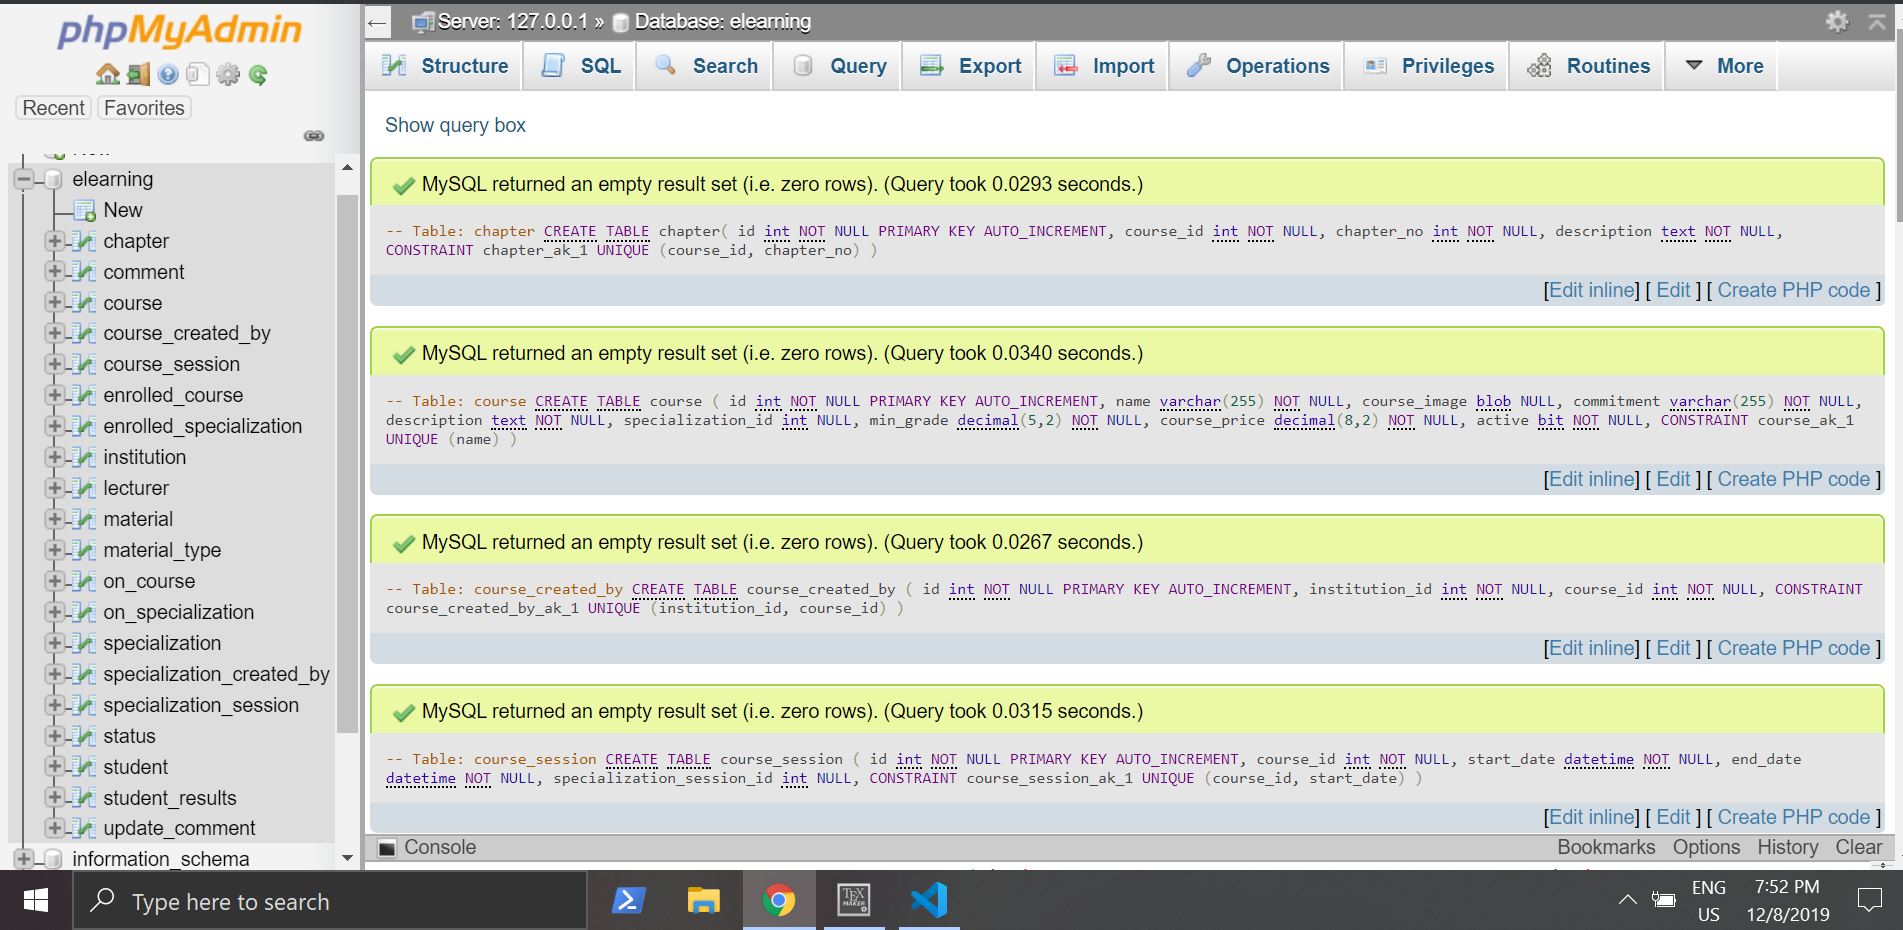
\includegraphics[width=0.8\textwidth]{images/create1.png}
	\caption{Có tất cả 20 bảng được tạo}
	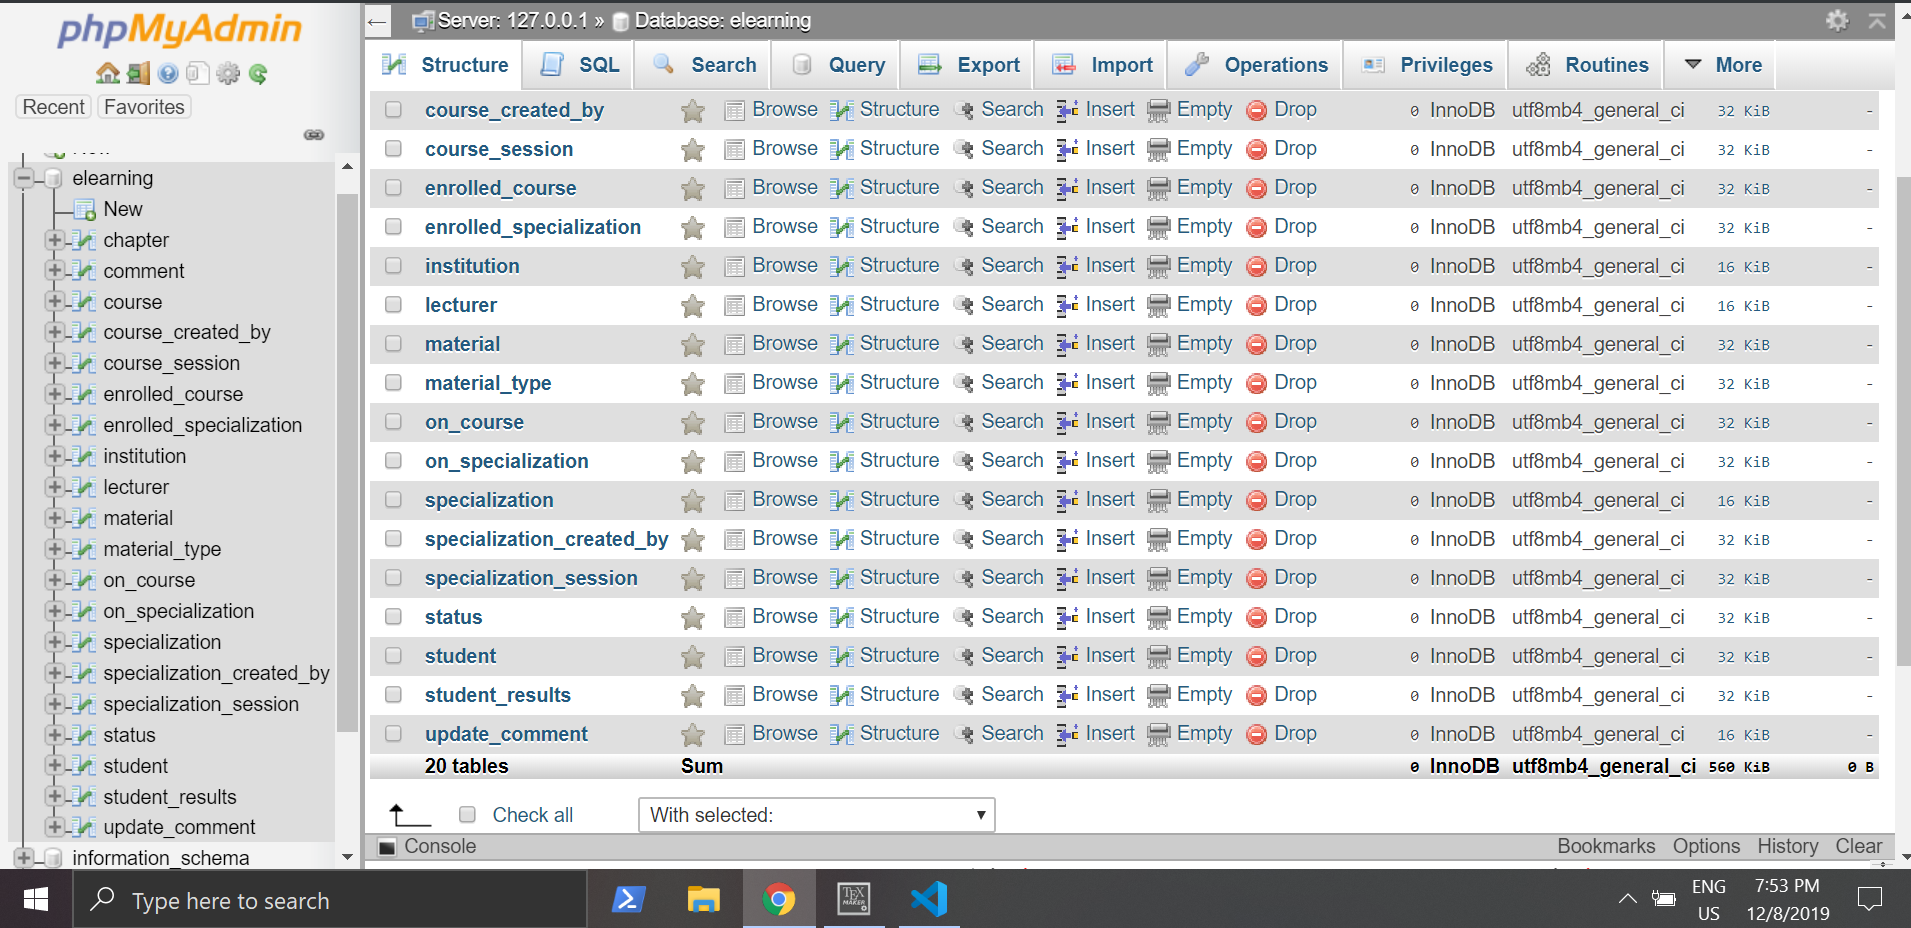
\includegraphics[width=0.8\textwidth]{images/create2.png}
\end{figure}
\textbf{b) Tạo ràng buộc:}
\begin{lstlisting}
-- foreign keys
-- Reference: chapter_course (table: chapter)
ALTER TABLE chapter ADD CONSTRAINT chapter_course
    FOREIGN KEY (course_id)
    REFERENCES course (id)
    ON DELETE CASCADE ;

-- Reference: course_created_by_course (table: course_created_by)
ALTER TABLE course_created_by ADD CONSTRAINT course_created_by_course
    FOREIGN KEY (course_id)
    REFERENCES course (id)
    ON DELETE CASCADE ;

-- Reference: course_created_by_institution (table: course_created_by)
ALTER TABLE course_created_by ADD CONSTRAINT course_created_by_institution
    FOREIGN KEY (institution_id)
    REFERENCES institution (id)
    ON DELETE CASCADE ;

-- Reference: course_session_course (table: course_session)
ALTER TABLE course_session ADD CONSTRAINT course_session_course
    FOREIGN KEY (course_id)
    REFERENCES course (id)
    ON DELETE CASCADE ;

-- Reference: course_session_specialization_session (table: course_session)
ALTER TABLE course_session ADD CONSTRAINT course_session_specialization_session
    FOREIGN KEY (specialization_session_id)
    REFERENCES specialization_session (id)
    ON DELETE SET NULL ;

-- Reference: course_specialization (table: course)
ALTER TABLE course ADD CONSTRAINT course_specialization
    FOREIGN KEY (specialization_id)
    REFERENCES specialization (id)
    ON DELETE SET NULL ;

-- Reference: enrolled_course_course_session (table: enrolled_course)
ALTER TABLE enrolled_course ADD CONSTRAINT enrolled_course_course_session
    FOREIGN KEY (course_session_id)
    REFERENCES course_session (id) 
    ON DELETE CASCADE ;

-- Reference: enrolled_course_status (table: enrolled_course)
ALTER TABLE enrolled_course ADD CONSTRAINT enrolled_course_status
    FOREIGN KEY (status_id)
    REFERENCES status (id)
    ON DELETE SET NULL ;

-- Reference: enrolled_course_student (table: enrolled_course)
ALTER TABLE enrolled_course ADD CONSTRAINT enrolled_course_student
    FOREIGN KEY (student_id)
    REFERENCES student (id)
    ON DELETE CASCADE ;

-- Reference: enrolled_specialization_specialization_session (table: enrolled_specialization)
ALTER TABLE enrolled_specialization ADD CONSTRAINT enrolled_specialization_specialization_session
    FOREIGN KEY (specialization_session_id)
    REFERENCES specialization_session (id)  
    ON DELETE CASCADE ;

-- Reference: enrolled_specialization_status (table: enrolled_specialization)
ALTER TABLE enrolled_specialization ADD CONSTRAINT enrolled_specialization_status
    FOREIGN KEY (status_id)
    REFERENCES status (id)  
    ON DELETE SET NULL ;

-- Reference: enrolled_specialization_student (table: enrolled_specialization)
ALTER TABLE enrolled_specialization ADD CONSTRAINT enrolled_specialization_student
    FOREIGN KEY (student_id)
    REFERENCES student (id)
    ON DELETE CASCADE ;

-- Reference: lecturer_institution (table: lecturer)
ALTER TABLE lecturer ADD CONSTRAINT lecturer_institution
    FOREIGN KEY (institution_id)
    REFERENCES institution (id)
    ON DELETE CASCADE ;

-- Reference: material_chapter (table: material)
ALTER TABLE material ADD CONSTRAINT material_chapter
    FOREIGN KEY (chapter_id)
    REFERENCES chapter (id)  
    ON DELETE CASCADE ;

-- Reference: material_material_type (table: material)
ALTER TABLE material ADD CONSTRAINT material_material_type
    FOREIGN KEY (material_type_id)
    REFERENCES material_type (id)
    ON DELETE SET NULL ;

-- Reference: on_course_course (table: on_course)
ALTER TABLE on_course ADD CONSTRAINT on_course_course
    FOREIGN KEY (course_id)
    REFERENCES course (id)
    ON DELETE CASCADE ;

-- Reference: on_course_lecturer (table: on_course)
ALTER TABLE on_course ADD CONSTRAINT on_course_lecturer
    FOREIGN KEY (lecturer_id)
    REFERENCES lecturer (id)
    ON DELETE CASCADE ;

-- Reference: on_specialization_lecturer (table: on_specialization)
ALTER TABLE on_specialization ADD CONSTRAINT on_specialization_lecturer
    FOREIGN KEY (lecturer_id)
    REFERENCES lecturer (id)
    ON DELETE CASCADE ;

-- Reference: on_specialization_specialization (table: on_specialization)
ALTER TABLE on_specialization ADD CONSTRAINT on_specialization_specialization
    FOREIGN KEY (specialization_id)
    REFERENCES specialization (id)  
    ON DELETE CASCADE ;

-- Reference: specialization_created_by_institution (table: specialization_created_by)
ALTER TABLE specialization_created_by ADD CONSTRAINT specialization_created_by_institution
    FOREIGN KEY (institution_id)
    REFERENCES institution (id)  
    ON DELETE CASCADE ;

-- Reference: specialization_created_by_specialization (table: specialization_created_by)
ALTER TABLE specialization_created_by ADD CONSTRAINT specialization_created_by_specialization
    FOREIGN KEY (specialization_id)
    REFERENCES specialization (id)  
    ON DELETE CASCADE ;

-- Reference: specialization_session_specialization (table: specialization_session)
ALTER TABLE specialization_session ADD CONSTRAINT specialization_session_specialization
    FOREIGN KEY (specialization_id)
    REFERENCES specialization (id)  
    ON DELETE CASCADE ;

-- Reference: student_results_enrolled_course (table: student_results)
ALTER TABLE student_results ADD CONSTRAINT student_results_enrolled_course
    FOREIGN KEY (enrolled_course_id)
    REFERENCES enrolled_course (id)  
    ON DELETE CASCADE ;

-- Reference: student_results_material (table: student_results)
ALTER TABLE student_results ADD CONSTRAINT student_results_material
    FOREIGN KEY (material_id)
    REFERENCES material (id)  
    ON DELETE CASCADE ;

-- Reference:
ALTER TABLE comment ADD CONSTRAINT comment_in_course
    FOREIGN KEY (course_id)
    REFERENCES course(id)
    ON DELETE CASCADE ;

-- Reference:
ALTER TABLE comment ADD CONSTRAINT comment_of_student
    FOREIGN KEY (student_id)
    REFERENCES student(id)
    ON DELETE CASCADE ;

-- Reference:
ALTER TABLE update_comment ADD CONSTRAINT last_comments_of_comment
    FOREIGN KEY (comment_id)
    REFERENCES comment(id)
    ON DELETE CASCADE ;

-- End of file.
\end{lstlisting}
\begin{figure}[h!]
	\centering
	\caption{Các ràng buộc khóa ngoại đều được tạo thành công}
	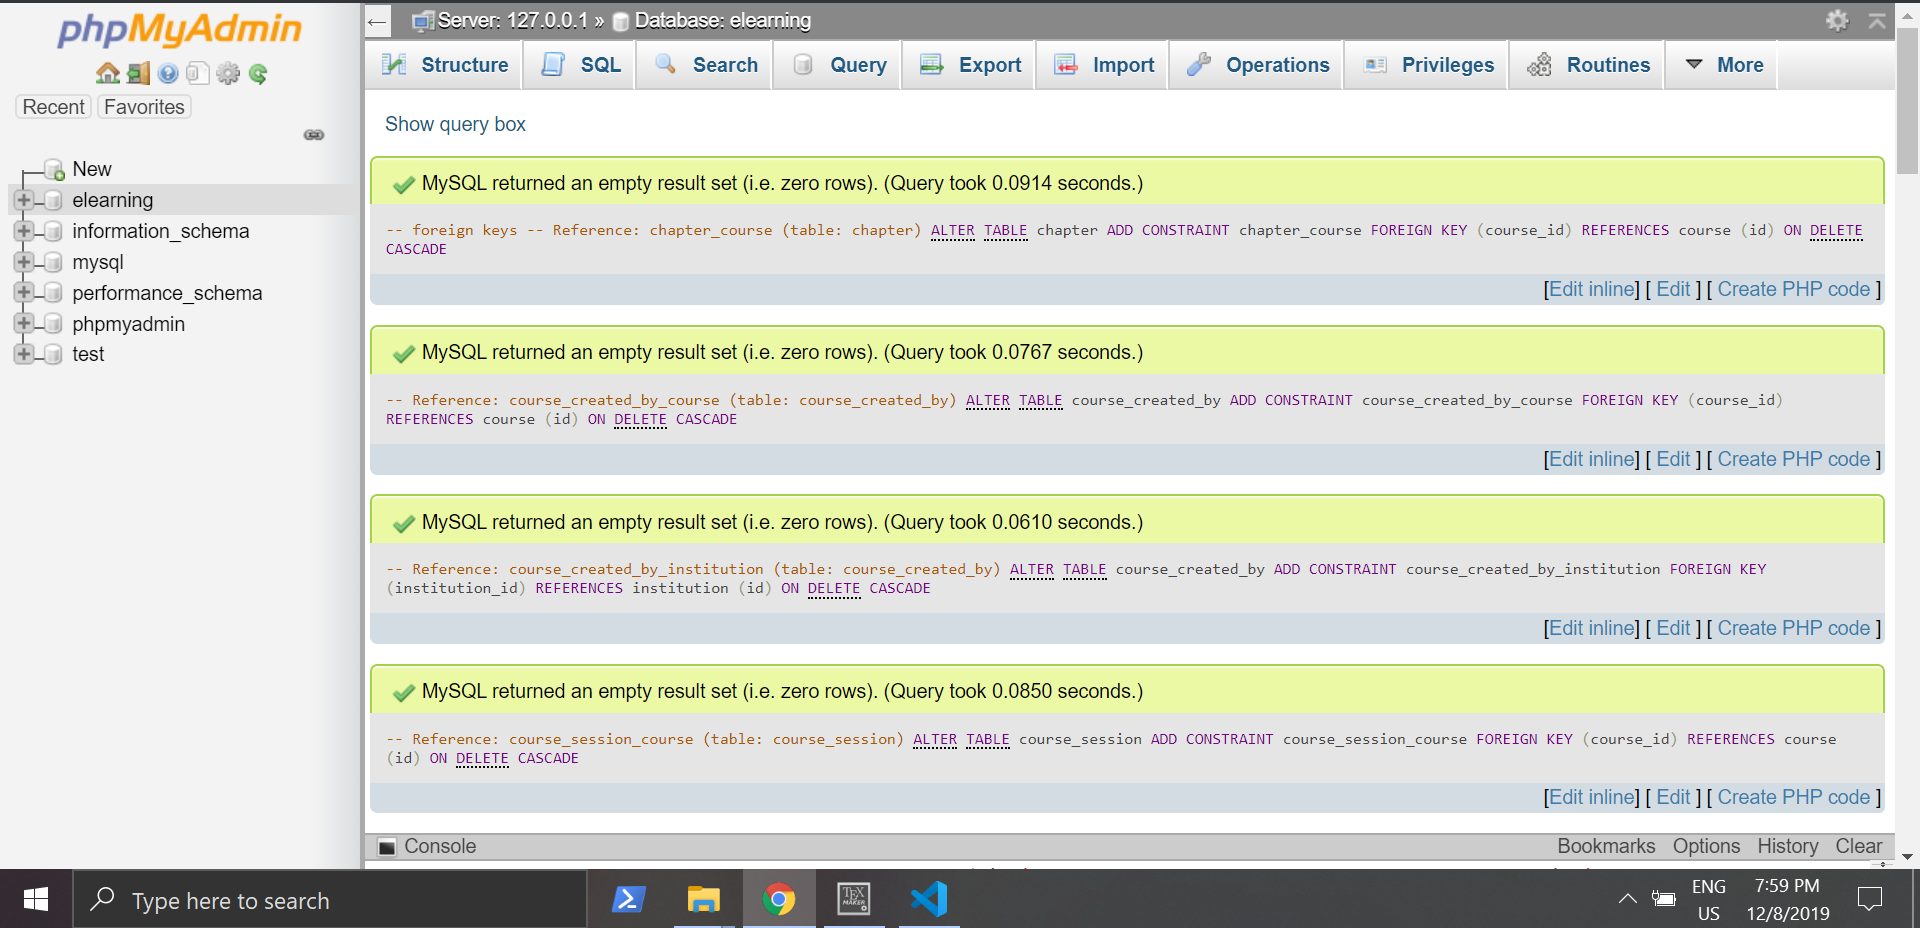
\includegraphics[width=0.8\textwidth]{images/fk.png}
\end{figure}
\subsection{Các lệnh tạo chỉ mục}
\begin{lstlisting}
-- INDEX: chapter

ALTER TABLE chapter ADD INDEX index_chapter(
    id,
    course_id,
    chapter_no
    );
-- INDEX: course

ALTER TABLE course ADD INDEX index_course(
    id ,
    name		,
    specialization_id	,
    course_price	,
    active	            
);

-- INDEX: course_created_by

ALTER TABLE course_created_by ADD INDEX (
    id,
    institution_id	,
    course_id			
);
-- INDEX: course_session

ALTER TABLE course_session ADD INDEX index_course_session(
    id   ,
    course_id   ,
    specialization_session_id  
);
-- INDEX: enrolled_course

ALTER TABLE enrolled_course ADD INDEX (
    id   ,
    student_id   ,
    course_session_id   
);
-- INDEX: enrolled_specialization

ALTER TABLE enrolled_specialization ADD INDEX index_enrolled_specialization(
    id   ,
    student_id   ,
    specialization_session_id   ,
    enrollment_date   ,
    status_id   
);


ALTER TABLE institution ADD INDEX index_institution (
    id  ,
    name  ,
    uname  ,
    pass  
);
-- INDEX: lecturer

ALTER TABLE lecturer ADD INDEX index_lecturer
(
    id  ,
    institution_id   
);
-- INDEX: material

ALTER TABLE material ADD INDEX index_material(
    id   ,
    chapter_id   ,
);
-- INDEX: material_type

ALTER TABLE material_type ADD INDEX index_material_type(
    id   ,
    type_name  
);

-- INDEX: on_course

ALTER TABLE on_course ADD INDEX index_on_course (
    id   ,
    lecturer_id   ,
    course_id   
);
-- INDEX: on_specialization

ALTER TABLE on_specialization ADD INDEX index_on_specialization(
    id   ,
    lecturer_id   ,
    specialization_id   
);
-- INDEX: specialization

ALTER TABLE specialization ADD INDEX index_specialization(
    id   ,
    name   
);
-- INDEX: specialization_created_by

ALTER TABLE specialization_created_by ADD INDEX index_specialization_created_by(
    id   ,
    institution_id   ,
    specialization_id   
);
-- INDEX: specialization_session

ALTER TABLE specialization_session ADD INDEX index_specialization_session(
    id   ,
    specialization_id   
);
-- INDEX: status

ALTER TABLE status ADD INDEX index_status(
    id  ,
    status_name   
);
-- INDEX: student

ALTER TABLE student ADD INDEX index_student(
    id   ,
    uname   ,
    pass   
);
-- INDEX: student_results

ALTER TABLE student_results ADD INDEX index_student_results(
    id   ,
    material_id   ,
    enrolled_course_id   ,
    score   
);
-- INDEX: comment

ALTER TABLE comment ADD INDEX index_comment(
	id  ,
	course_id  ,
	student_id  
);
\end{lstlisting}
\newpage
\subsection{Các lệnh thêm dữ liệu vào bảng}
\begin{lstlisting}
-- Institution
INSERT INTO `institution` VALUES(NULL, 'University of Oxford', 'Oxford, England, United Kingdom', 'oxford@gmail.com', '123456');
INSERT INTO `institution` VALUES(NULL, 'University of Cambridge', 'Cambridge, England, United Kingdom', 'cambridge@gmail.com', '123456');
INSERT INTO `institution` VALUES(NULL, 'University of Sheffield', 'Sheffield, South Yorkshire, England', 'sheffield@gmail.com', '123456');

INSERT INTO `institution` VALUES(NULL, 'Massachusetts Institute of Technology', 'Cambridge, Massachusetts, United States', 'mit@gmail.com', '123456');
INSERT INTO `institution` VALUES(NULL, 'Harvard University', 'Cambridge, Massachusetts, United States', 'harvard@gmail.com', '123456');
INSERT INTO `institution` VALUES(NULL, 'Stanford University', 'Stanford, California, United States', 'stanford@gmail.com', '123456');

INSERT INTO `institution` VALUES(NULL, 'The University of Tokyo', 'Bunkyoo, Tokyo, Japan', 'todai@gmail.com', '123456');
INSERT INTO `institution` VALUES(NULL, 'Tsinghua University', 'Haidian District, Beijing, Peoples Republic of China', 'tsinghua@gmail.com', '123456');
INSERT INTO `institution` VALUES(NULL, 'National University of Singapore', 'Singapore', 'nus@gmail.com', '123456');
INSERT INTO `institution` VALUES(NULL, 'HCMC University of Technology', '268 Ly Thuong Kiet St., Dist.10, Ho Chi Minh City, Vietnam','hcmut@gmail.com', '123456');
--

-- Lecturer
INSERT INTO `lecturer` VALUES(NULL, 'Jeff', 'Leek', 'Associate Professor', 1);
INSERT INTO `lecturer` VALUES(NULL, 'Brian', 'Caffo', 'Professor', 1);
INSERT INTO `lecturer` VALUES(NULL, 'Roger', 'Peng', 'Associate Professor', 1);
INSERT INTO `lecturer` VALUES(NULL, 'Tim', 'Roughgarden', 'Professor', 1);
INSERT INTO `lecturer` VALUES(NULL, 'Brent', 'Hecht', 'Assistant Professor',1);

INSERT INTO `lecturer` VALUES(NULL, 'Jeff', 'Leek', 'Associate Professor', 3);
INSERT INTO `lecturer` VALUES(NULL, 'Brian', 'Caffo', 'Professor', 3);
INSERT INTO `lecturer` VALUES(NULL, 'Roger', 'Peng', 'Associate Professor', 3);
INSERT INTO `lecturer` VALUES(NULL, 'Tim', 'Roughgarden', 'Professor', 3);
INSERT INTO `lecturer` VALUES(NULL, 'Brent', 'Hecht', 'Assistant Professor',3);

INSERT INTO `lecturer` VALUES(NULL, 'Tess', 'Wilkinson-Ryan', 'Associate Professor', 5);
INSERT INTO `lecturer` VALUES(NULL, 'Philip', 'Peck', 'Associate Professor',5);
INSERT INTO `lecturer` VALUES(NULL, 'Alex', 'Aklson', 'Data Scientist', 5);
INSERT INTO `lecturer` VALUES(NULL, 'Nigel', 'Saul', 'Professor', 5);
INSERT INTO `lecturer` VALUES(NULL, 'Candy', 'Lee', 'Professor', 5);

INSERT INTO `lecturer` VALUES(NULL, 'Tess', 'Wilkinson-Ryan', 'Associate Professor', 6);
INSERT INTO `lecturer` VALUES(NULL, 'Philip', 'Peck', 'Associate Professor',6);
INSERT INTO `lecturer` VALUES(NULL, 'Alex', 'Aklson', 'Data Scientist', 6);
INSERT INTO `lecturer` VALUES(NULL, 'Nigel', 'Saul', 'Professor', 6);
INSERT INTO `lecturer` VALUES(NULL, 'Candy', 'Lee', 'Professor', 6);

INSERT INTO `lecturer` VALUES(NULL, 'Chi', 'Truong Quynh', 'Lecturer', 10);
INSERT INTO `lecturer` VALUES(NULL, 'Phung', 'Nguyen Hua', 'Associate Professor', 10);
INSERT INTO `lecturer` VALUES(NULL, 'Nam', 'Thoai', 'Professor', 10);
INSERT INTO `lecturer` VALUES(NULL, 'Ty', 'Nguyen Huu Ky', 'Lecturer', 10);
INSERT INTO `lecturer` VALUES(NULL, 'Lai', 'Nguyen Le Duy', 'Lecturer', 10);

-- Specialization/Course
--
INSERT INTO `specialization` VALUES(NULL, 'Introduction to Data Mining', 'Learn to apply data science methods and techniques, and acquire analysis skills.', 6.0, 1, 4);
INSERT INTO `course` VALUES(NULL, 'Learn Python 3', NULL, 'We remains committed to providing certificate', 'Learn to use Python 3', 1, 7.5, 19.0, 1);
INSERT INTO `course` VALUES(NULL, 'Advanced Algorithms', NULL, 'We remains committed to providing certificate', 'Learn algorithms', 1, 7.5, 33.0, 1);
INSERT INTO `course` VALUES(NULL, 'DFS Hadoop', NULL, 'We remains committed to providing certificate', 'Learn hadoop', 1, 7.5, 15.0, 1);
INSERT INTO `course` VALUES(NULL, 'HIV/AIDS Victim Data Mining Project', NULL, 'We remains committed to providing certificate', 'Final project', 1, 9.5, 35.0, 1);
--
INSERT INTO `specialization` VALUES(NULL, 'Mathematics for Machine Learning', 'Learn about the prerequisite mathematics for applications in data science and machine learning.', 10.0, 1, 3);
INSERT INTO `course` VALUES(NULL, 'Linear Algebra', NULL, 'We remains committed to providing certificate', 'Learn linear algebra', 2, 5.0, 21.0, 1);
INSERT INTO `course` VALUES(NULL, 'Multivariable Calculus', NULL, 'We remains committed to providing certificate', 'Learn multivariable calculus', 2, 5.0, 19.0, 1);
INSERT INTO `course` VALUES(NULL, 'PCA', NULL, 'We remains committed to providing certificate', 'Learn principal component analysis', 2, 8.0, 30.0, 1);
--
INSERT INTO `specialization` VALUES(NULL, 'Introduction to Deep Learning', 'Neural Networks for Computer Vision, Time Series Forecasting, NLP, GANs', 13.0, 1, 4);
INSERT INTO `course` VALUES(NULL, 'Introduction to Neural Networks', NULL, 'We remains committed to providing certificate', 'Learn neural networks', 3, 7.0, 25.0, 1);
INSERT INTO `course` VALUES(NULL, 'Introduction to Computer Vision', NULL, 'We remains committed to providing certificate', 'Learn Python OpenCV', 3, 9.0, 27.0, 1);
INSERT INTO `course` VALUES(NULL, 'Decision Tree', NULL, 'We remains committed to providing certificate', 'Learn decision tree', 3, 9.0, 30.0, 1);
INSERT INTO `course` VALUES(NULL, 'Support Vector Machine', NULL, 'We remains committed to providing certificate', 'Learn SVM', 3, 9.0, 30.0, 1);
--
INSERT INTO `course` VALUES(NULL, 'Anh Van 1', NULL, 'We remains committed to providing certificate', 'Learn English', NULL, 5.0, 50.0, 1);
INSERT INTO `course` VALUES(NULL, 'Anh Van 2', NULL, 'We remains committed to providing certificate', 'Learn English', NULL, 5.0, 50.0, 1);
INSERT INTO `course` VALUES(NULL, 'Anh Van 3', NULL, 'We remains committed to providing certificate', 'Learn English', NULL, 5.0, 50.0, 1);
INSERT INTO `course` VALUES(NULL, 'Anh Van 4', NULL, 'We remains committed to providing certificate', 'Learn English', NULL, 5.0, 50.0, 1);
INSERT INTO `course` VALUES(NULL, 'Giai tich 1', NULL, 'We remains committed to providing certificate', 'Learn mathematical analysis', NULL, 5.0, 100.0, 1);
INSERT INTO `course` VALUES(NULL, 'Giai tich 2', NULL, 'We remains committed to providing certificate', 'Learn mathematical analysis', NULL, 5.0, 100.0, 1);
INSERT INTO `course` VALUES(NULL, 'Giai tich 3', NULL, 'We remains committed to providing certificate', 'Learn mathematical analysis', NULL, 5.0, 100.0, 1);
INSERT INTO `course` VALUES(NULL, 'Vat Ly 1', NULL, 'We remains committed to providing certificate', 'Learn physics', NULL, 5.0, 100.0, 1);
INSERT INTO `course` VALUES(NULL, 'Vat Ly 2', NULL, 'We remains committed to providing certificate', 'Learn physics', NULL, 5.0, 100.0, 1);
INSERT INTO `course` VALUES(NULL, 'Hoa Dai cuong', NULL, 'We remains committed to providing certificate', 'Learn chemistry', NULL, 5.0, 75.0, 1);
INSERT INTO `course` VALUES(NULL, 'Nhap mon Dien toan', NULL, 'We remains committed to providing certificate', 'Learn computer science', NULL, 5.0, 75.0, 1);
INSERT INTO `course` VALUES(NULL, 'Cau truc roi rac cho Khoa hoc May tinh', NULL, 'We remains committed to providing certificate', 'Learn computer science', NULL, 5.0, 100.0, 1);
INSERT INTO `course` VALUES(NULL, 'Dai so tuyen tinh', NULL, 'We remains committed to providing certificate', 'Learn linear algebra', NULL, 5.0, 75.0, 1);
INSERT INTO `course` VALUES(NULL, 'He thong so', NULL, 'We remains committed to providing certificate', 'Learn computer science', NULL, 5.0, 100.0, 1);
INSERT INTO `course` VALUES(NULL, 'Ky thuat lap trinh', NULL, 'We remains committed to providing certificate', 'Learn computer science', NULL, 5.0, 100.0, 1);
INSERT INTO `course` VALUES(NULL, 'Thi nghiem Vat Ly', NULL, 'We remains committed to providing certificate', 'Learn physics', NULL, 5.0, 25.0, 1);
INSERT INTO `course` VALUES(NULL, 'Phuong phap tinh', NULL, 'We remains committed to providing certificate', 'Learn calculus method', NULL, 5.0, 75.0, 1);
INSERT INTO `course` VALUES(NULL, 'Cau truc du lieu va Giai thuat', NULL, 'We remains committed to providing certificate', 'Learn computer science', NULL, 5.0, 100.0, 1);
INSERT INTO `course` VALUES(NULL, 'Lap trinh Huong doi tuong', NULL, 'We remains committed to providing certificate', 'Learn computer science', NULL, 5.0, 100.0, 1);
INSERT INTO `course` VALUES(NULL, 'Kien truc May tinh', NULL, 'We remains committed to providing certificate', 'Learn computer science', NULL, 5.0, 100.0, 1);
INSERT INTO `course` VALUES(NULL, 'Mo hinh hoa Toan hoc', NULL, 'We remains committed to providing certificate', 'Learn computer science', NULL, 5.0, 75.0, 1);
INSERT INTO `course` VALUES(NULL, 'He dieu hanh', NULL, 'We remains committed to providing certificate', 'Learn computer science', NULL, 5.0, 75.0, 1);
INSERT INTO `course` VALUES(NULL, 'Cong nghe phan mem', NULL, 'We remains committed to providing certificate', 'Learn computer science', NULL, 5.0, 75.0, 1);
INSERT INTO `course` VALUES(NULL, 'Xac suat va Thong ke', NULL, 'We remains committed to providing certificate', 'Learn probability and statistics', NULL, 5.0, 75.0, 1);
INSERT INTO `course` VALUES(NULL, 'Nguyen ly ngon ngu lap trinh', NULL, 'We remains committed to providing certificate', 'Learn computer science', NULL, 5.0, 100.0, 1);
INSERT INTO `course` VALUES(NULL, 'Tinh toan song song', NULL, 'We remains committed to providing certificate', 'Learn computer science', NULL, 5.0, 100.0, 1);
INSERT INTO `course` VALUES(NULL, 'He co so du lieu', NULL, 'We remains committed to providing certificate', 'Learn computer science', NULL, 5.0, 100.0, 1);
INSERT INTO `course` VALUES(NULL, 'Mang may tinh', NULL, 'We remains committed to providing certificate', 'Learn computer science', NULL, 5.0, 100.0, 1);

-- course create by
INSERT INTO `course_created_by` VALUES(NULL, 10, 12);
INSERT INTO `course_created_by` VALUES(NULL, 10, 13);
INSERT INTO `course_created_by` VALUES(NULL, 10, 14);
INSERT INTO `course_created_by` VALUES(NULL, 10, 15);
INSERT INTO `course_created_by` VALUES(NULL, 10, 16);
INSERT INTO `course_created_by` VALUES(NULL, 10, 17);
INSERT INTO `course_created_by` VALUES(NULL, 10, 18);
INSERT INTO `course_created_by` VALUES(NULL, 10, 19);
INSERT INTO `course_created_by` VALUES(NULL, 10, 20);
INSERT INTO `course_created_by` VALUES(NULL, 10, 21);
INSERT INTO `course_created_by` VALUES(NULL, 10, 22);
INSERT INTO `course_created_by` VALUES(NULL, 10, 23);
INSERT INTO `course_created_by` VALUES(NULL, 10, 24);
INSERT INTO `course_created_by` VALUES(NULL, 10, 25);
INSERT INTO `course_created_by` VALUES(NULL, 10, 26);
INSERT INTO `course_created_by` VALUES(NULL, 10, 27);
INSERT INTO `course_created_by` VALUES(NULL, 10, 28);
INSERT INTO `course_created_by` VALUES(NULL, 10, 29);
INSERT INTO `course_created_by` VALUES(NULL, 10, 30);
INSERT INTO `course_created_by` VALUES(NULL, 10, 31);
INSERT INTO `course_created_by` VALUES(NULL, 10, 32);
INSERT INTO `course_created_by` VALUES(NULL, 10, 33);
INSERT INTO `course_created_by` VALUES(NULL, 10, 34);
INSERT INTO `course_created_by` VALUES(NULL, 10, 35);
INSERT INTO `course_created_by` VALUES(NULL, 10, 36);
INSERT INTO `course_created_by` VALUES(NULL, 10, 37);
INSERT INTO `course_created_by` VALUES(NULL, 10, 38);
INSERT INTO `course_created_by` VALUES(NULL, 10, 39);

INSERT INTO `course_created_by` VALUES(NULL, 1, 1);
INSERT INTO `course_created_by` VALUES(NULL, 1, 2);
INSERT INTO `course_created_by` VALUES(NULL, 1, 3);
INSERT INTO `course_created_by` VALUES(NULL, 1, 4);

INSERT INTO `course_created_by` VALUES(NULL, 3, 5);
INSERT INTO `course_created_by` VALUES(NULL, 3, 6);
INSERT INTO `course_created_by` VALUES(NULL, 3, 7);

INSERT INTO `course_created_by` VALUES(NULL, 5, 8);
INSERT INTO `course_created_by` VALUES(NULL, 5, 9);
INSERT INTO `course_created_by` VALUES(NULL, 5, 10);
INSERT INTO `course_created_by` VALUES(NULL, 5, 11);

-- specialization create by
INSERT INTO `specialization_created_by` VALUES(NULL, 1, 1);
INSERT INTO `specialization_created_by` VALUES(NULL, 3, 2);
INSERT INTO `specialization_created_by` VALUES(NULL, 5, 3);

-- on course
INSERT INTO `on_course` VALUES(NULL, 21, 12);
INSERT INTO `on_course` VALUES(NULL, 21, 13);
INSERT INTO `on_course` VALUES(NULL, 21, 14);
INSERT INTO `on_course` VALUES(NULL, 21, 15);
INSERT INTO `on_course` VALUES(NULL, 22, 16);
INSERT INTO `on_course` VALUES(NULL, 22, 17);
INSERT INTO `on_course` VALUES(NULL, 22, 18);
INSERT INTO `on_course` VALUES(NULL, 22, 19);
INSERT INTO `on_course` VALUES(NULL, 22, 20);
INSERT INTO `on_course` VALUES(NULL, 22, 21);
INSERT INTO `on_course` VALUES(NULL, 23, 22);
INSERT INTO `on_course` VALUES(NULL, 23, 23);
INSERT INTO `on_course` VALUES(NULL, 23, 24);
INSERT INTO `on_course` VALUES(NULL, 23, 25);
INSERT INTO `on_course` VALUES(NULL, 23, 26);
INSERT INTO `on_course` VALUES(NULL, 23, 27);
INSERT INTO `on_course` VALUES(NULL, 24, 28);
INSERT INTO `on_course` VALUES(NULL, 24, 29);
INSERT INTO `on_course` VALUES(NULL, 24, 30);
INSERT INTO `on_course` VALUES(NULL, 24, 31);
INSERT INTO `on_course` VALUES(NULL, 25, 32);
INSERT INTO `on_course` VALUES(NULL, 25, 33);
INSERT INTO `on_course` VALUES(NULL, 25, 34);
INSERT INTO `on_course` VALUES(NULL, 25, 35);
INSERT INTO `on_course` VALUES(NULL, 25, 36);
INSERT INTO `on_course` VALUES(NULL, 25, 37);
INSERT INTO `on_course` VALUES(NULL, 25, 38);
INSERT INTO `on_course` VALUES(NULL, 25, 39);

INSERT INTO `on_course` VALUES(NULL, 21, 31);
INSERT INTO `on_course` VALUES(NULL, 21, 32);
INSERT INTO `on_course` VALUES(NULL, 21, 33);
INSERT INTO `on_course` VALUES(NULL, 21, 34);
INSERT INTO `on_course` VALUES(NULL, 21, 35);
INSERT INTO `on_course` VALUES(NULL, 21, 36);
INSERT INTO `on_course` VALUES(NULL, 21, 37);
INSERT INTO `on_course` VALUES(NULL, 21, 38);
INSERT INTO `on_course` VALUES(NULL, 21, 39);

INSERT INTO `on_course` VALUES(NULL, 22, 24);
INSERT INTO `on_course` VALUES(NULL, 22, 25);
INSERT INTO `on_course` VALUES(NULL, 22, 26);
INSERT INTO `on_course` VALUES(NULL, 22, 27);
INSERT INTO `on_course` VALUES(NULL, 22, 28);
INSERT INTO `on_course` VALUES(NULL, 22, 29);
INSERT INTO `on_course` VALUES(NULL, 22, 30);
INSERT INTO `on_course` VALUES(NULL, 22, 31);
INSERT INTO `on_course` VALUES(NULL, 22, 32);
INSERT INTO `on_course` VALUES(NULL, 22, 33);
INSERT INTO `on_course` VALUES(NULL, 22, 34);
INSERT INTO `on_course` VALUES(NULL, 22, 35);

-- chapter
INSERT INTO `chapter` VALUES(NULL, 38, 1, 'Introduction to Database Systems');
INSERT INTO `chapter` VALUES(NULL, 38, 2, 'Database System Concepts And Architecture');
INSERT INTO `chapter` VALUES(NULL, 38, 3, 'Entity Relationship Model');
INSERT INTO `chapter` VALUES(NULL, 38, 4, 'Extended Entity Relationship Model');
INSERT INTO `chapter` VALUES(NULL, 38, 5, 'Relational Data Model And Relational Mapping');
INSERT INTO `chapter` VALUES(NULL, 38, 6, 'Relational Algebra');
INSERT INTO `chapter` VALUES(NULL, 38, 7, 'SQL');
INSERT INTO `chapter` VALUES(NULL, 38, 8, 'FD1');
INSERT INTO `chapter` VALUES(NULL, 38, 9, 'DBS');

INSERT INTO `chapter` VALUES(NULL, 36, 1, 'Introduction');
INSERT INTO `chapter` VALUES(NULL, 36, 2, 'Lexical Analysis');
INSERT INTO `chapter` VALUES(NULL, 36, 3, 'Syntax Analysis');
INSERT INTO `chapter` VALUES(NULL, 36, 4, 'OOP and Scala');
INSERT INTO `chapter` VALUES(NULL, 36, 5, 'Functional Programming');
INSERT INTO `chapter` VALUES(NULL, 36, 6, 'Abstract Syntax Tree');
INSERT INTO `chapter` VALUES(NULL, 36, 7, 'Name');
INSERT INTO `chapter` VALUES(NULL, 36, 8, 'Type');
INSERT INTO `chapter` VALUES(NULL, 36, 9, 'Sequence Control');
INSERT INTO `chapter` VALUES(NULL, 36, 10, 'Control Abstraction');
INSERT INTO `chapter` VALUES(NULL, 36, 11, 'JVM');
INSERT INTO `chapter` VALUES(NULL, 36, 12, 'JVM Code Generation');

-- material type
INSERT INTO `material_type` VALUES(NULL, 'Video');
INSERT INTO `material_type` VALUES(NULL, 'Slide');
INSERT INTO `material_type` VALUES(NULL, 'Tutorial');
INSERT INTO `material_type` VALUES(NULL, 'Lab');
INSERT INTO `material_type` VALUES(NULL, 'Exercise');
INSERT INTO `material_type` VALUES(NULL, 'Assignment');
INSERT INTO `material_type` VALUES(NULL, 'Quiz');
INSERT INTO `material_type` VALUES(NULL, 'Survey');
INSERT INTO `material_type` VALUES(NULL, 'Outline');

-- materal
INSERT INTO `material` VALUES(NULL, 10, 1, 8, 'http://e-learning.hcmut.edu.vn/mod/feedback/view.php?id=347990', 1, 10);
INSERT INTO `material` VALUES(NULL, 10, 2, 2, 'http://e-learning.hcmut.edu.vn/mod/feedback/view.php?id=347990', 0, 0);
INSERT INTO `material` VALUES(NULL, 10, 3, 5, 'http://e-learning.hcmut.edu.vn/mod/feedback/view.php?id=347990', 1, 10);

INSERT INTO `material` VALUES(NULL, 11, 1, 1, 'http://e-learning.hcmut.edu.vn/mod/feedback/view.php?id=347990', 1, 10);
INSERT INTO `material` VALUES(NULL, 11, 2, 2, 'http://e-learning.hcmut.edu.vn/mod/feedback/view.php?id=347990', 0, 0);
INSERT INTO `material` VALUES(NULL, 11, 3, 3, 'http://e-learning.hcmut.edu.vn/mod/feedback/view.php?id=347990', 1, 10);
INSERT INTO `material` VALUES(NULL, 11, 4, 5, 'http://e-learning.hcmut.edu.vn/mod/feedback/view.php?id=347990', 1, 10);
INSERT INTO `material` VALUES(NULL, 11, 5, 7, 'http://e-learning.hcmut.edu.vn/mod/feedback/view.php?id=347990', 1, 10);

INSERT INTO `material` VALUES(NULL, 12, 1, 1, 'http://e-learning.hcmut.edu.vn/mod/feedback/view.php?id=347990', 1, 10);
INSERT INTO `material` VALUES(NULL, 12, 2, 2, 'http://e-learning.hcmut.edu.vn/mod/feedback/view.php?id=347990', 0, 0);
INSERT INTO `material` VALUES(NULL, 12, 3, 3, 'http://e-learning.hcmut.edu.vn/mod/feedback/view.php?id=347990', 1, 10);
INSERT INTO `material` VALUES(NULL, 12, 4, 5, 'http://e-learning.hcmut.edu.vn/mod/feedback/view.php?id=347990', 1, 10);
INSERT INTO `material` VALUES(NULL, 12, 5, 7, 'http://e-learning.hcmut.edu.vn/mod/feedback/view.php?id=347990', 1, 10);
INSERT INTO `material` VALUES(NULL, 12, 6, 7, 'http://e-learning.hcmut.edu.vn/mod/feedback/view.php?id=347990', 1, 10);

INSERT INTO `material` VALUES(NULL, 13, 1, 1, 'http://e-learning.hcmut.edu.vn/mod/feedback/view.php?id=347990', 1, 10);
INSERT INTO `material` VALUES(NULL, 13, 2, 2, 'http://e-learning.hcmut.edu.vn/mod/feedback/view.php?id=347990', 0, 0);
INSERT INTO `material` VALUES(NULL, 13, 3, 3, 'http://e-learning.hcmut.edu.vn/mod/feedback/view.php?id=347990', 1, 10);
INSERT INTO `material` VALUES(NULL, 13, 4, 5, 'http://e-learning.hcmut.edu.vn/mod/feedback/view.php?id=347990', 1, 10);
INSERT INTO `material` VALUES(NULL, 13, 5, 7, 'http://e-learning.hcmut.edu.vn/mod/feedback/view.php?id=347990', 1, 10);
INSERT INTO `material` VALUES(NULL, 13, 6, 1, 'http://e-learning.hcmut.edu.vn/mod/feedback/view.php?id=347990', 1, 10);
INSERT INTO `material` VALUES(NULL, 13, 7, 2, 'http://e-learning.hcmut.edu.vn/mod/feedback/view.php?id=347990', 0, 0);
INSERT INTO `material` VALUES(NULL, 13, 8, 3, 'http://e-learning.hcmut.edu.vn/mod/feedback/view.php?id=347990', 1, 10);
INSERT INTO `material` VALUES(NULL, 13, 9, 7, 'http://e-learning.hcmut.edu.vn/mod/feedback/view.php?id=347990', 1, 10);

INSERT INTO `material` VALUES(NULL, 15, 1, 1, 'http://e-learning.hcmut.edu.vn/mod/feedback/view.php?id=347990', 1, 10);
INSERT INTO `material` VALUES(NULL, 15, 2, 2, 'http://e-learning.hcmut.edu.vn/mod/feedback/view.php?id=347990', 0, 0);
INSERT INTO `material` VALUES(NULL, 15, 3, 3, 'http://e-learning.hcmut.edu.vn/mod/feedback/view.php?id=347990', 1, 10);
INSERT INTO `material` VALUES(NULL, 15, 4, 5, 'http://e-learning.hcmut.edu.vn/mod/feedback/view.php?id=347990', 1, 10);
INSERT INTO `material` VALUES(NULL, 15, 5, 7, 'http://e-learning.hcmut.edu.vn/mod/feedback/view.php?id=347990', 1, 10);
INSERT INTO `material` VALUES(NULL, 15, 6, 7, 'http://e-learning.hcmut.edu.vn/mod/feedback/view.php?id=347990', 1, 10);

INSERT INTO `material` VALUES(NULL, 16, 1, 1, 'http://e-learning.hcmut.edu.vn/mod/feedback/view.php?id=347990', 1, 10);
INSERT INTO `material` VALUES(NULL, 16, 2, 2, 'http://e-learning.hcmut.edu.vn/mod/feedback/view.php?id=347990', 0, 0);
INSERT INTO `material` VALUES(NULL, 16, 3, 3, 'http://e-learning.hcmut.edu.vn/mod/feedback/view.php?id=347990', 1, 10);
INSERT INTO `material` VALUES(NULL, 16, 4, 5, 'http://e-learning.hcmut.edu.vn/mod/feedback/view.php?id=347990', 1, 10);
INSERT INTO `material` VALUES(NULL, 16, 5, 7, 'http://e-learning.hcmut.edu.vn/mod/feedback/view.php?id=347990', 1, 10);

INSERT INTO `material` VALUES(NULL, 17, 1, 1, 'http://e-learning.hcmut.edu.vn/mod/feedback/view.php?id=347990', 1, 10);
INSERT INTO `material` VALUES(NULL, 17, 2, 2, 'http://e-learning.hcmut.edu.vn/mod/feedback/view.php?id=347990', 0, 0);
INSERT INTO `material` VALUES(NULL, 17, 3, 3, 'http://e-learning.hcmut.edu.vn/mod/feedback/view.php?id=347990', 1, 10);
INSERT INTO `material` VALUES(NULL, 17, 4, 5, 'http://e-learning.hcmut.edu.vn/mod/feedback/view.php?id=347990', 1, 10);
INSERT INTO `material` VALUES(NULL, 17, 5, 7, 'http://e-learning.hcmut.edu.vn/mod/feedback/view.php?id=347990', 1, 10);

-- status
INSERT INTO `status` VALUES(NULL, 'achieving');
INSERT INTO `status` VALUES(NULL, 'achieved');

-- student
INSERT INTO `student` VALUES(NULL, 'An', 'Nguyen Pham Duy', NULL, 'nguyenphamduyan430@gmail.com', '12345678', 'HCMC');
INSERT INTO `student` VALUES(NULL, 'Anh', 'Nguyen Cong', NULL, 'nguyenconganh477@gmail.com', '12345678', 'HCMC');
INSERT INTO `student` VALUES(NULL, 'Tai', 'Duong Van', NULL, 'duongvantai001@gmail.com', '12345678', 'HCMC');
INSERT INTO `student` VALUES(NULL, 'Hoa', 'Pham', NULL, 'phamhoa440@gmail.com', '12345678', 'HCMC');

INSERT INTO `student` VALUES(NULL, 'An', 'Nguyen Thanh Khanh', NULL, 'nguyenthanhkhanhan433@gmail.com', '12345678', 'HCMC');
INSERT INTO `student` VALUES(NULL, 'Anh', 'Bui Ba', NULL, 'buibaanh447@gmail.com', '12345678', 'HCMC');
INSERT INTO `student` VALUES(NULL, 'Anh', 'La Quoc', NULL, 'laquocanh465@gmail.com', '12345678', 'HCMC');
INSERT INTO `student` VALUES(NULL, 'Anh', 'Nguyen Trong', NULL, 'nguyentronganh500@gmail.com', '12345678', 'HCMC');

INSERT INTO `student` VALUES(NULL, 'Dat', 'Phan Thanh', NULL, 'phanthanhdat984@gmail.com', '12345678', 'HCMC');
INSERT INTO `student` VALUES(NULL, 'Dang', 'Nguyen Tran Minh Dang', NULL, 'nguyentranminhdang014@gmail.com', '12345678', 'HCMC');
INSERT INTO `student` VALUES(NULL, 'Dang', 'Tran Hai Dang', NULL, 'tranhaidang016@gmail.com', '12345678', 'HCMC');
INSERT INTO `student` VALUES(NULL, 'De', 'Chung Minh', NULL, 'chungminhde020@gmail.com', '12345678', 'HCMC');

INSERT INTO `student` VALUES(NULL, 'Phu', 'Huynh Quoc', NULL, 'huynhquocphu638@gmail.com', '12345678', 'HCMC');
INSERT INTO `student` VALUES(NULL, 'Phu', 'Nguyen Duc', NULL, 'nguyenducphu234@gmail.com', '12345678', 'HCMC');
INSERT INTO `student` VALUES(NULL, 'Phuc', 'Dang Hoang', NULL, 'danghoangphuc657@gmail.com', '12345678', 'HCMC');
INSERT INTO `student` VALUES(NULL, 'Quang', 'Tran Thanh', NULL, 'tranthanhquang802@gmail.com', '12345678', 'HCMC');

INSERT INTO `student` VALUES(NULL, 'Truong', 'Dang Cao Xuan', NULL, 'dangcaoxuantruong737@gmail.com', '12345678', 'HCMC');
INSERT INTO `student` VALUES(NULL, 'Truong', 'Trinh Duc', NULL, 'trinhductruong759@gmail.com', '12345678', 'HCMC');
INSERT INTO `student` VALUES(NULL, 'Van', 'Dang Anh', NULL, 'danganhvan913@gmail.com', '12345678', 'HCMC');
INSERT INTO `student` VALUES(NULL, 'Vy', 'Lam Chi', NULL, 'lamchivi993@gmail.com', '12345678', 'HCMC');

-- course session

INSERT INTO `course_session` VALUES(NULL, 12, '2019-01-01 00:00:00', '2019-03-01 00:00:00', NULL);
INSERT INTO `course_session` VALUES(NULL, 12, '2019-04-01 00:00:00', '2019-06-01 00:00:00', NULL);
INSERT INTO `course_session` VALUES(NULL, 12, '2019-08-01 00:00:00', '2019-10-01 00:00:00', NULL);

INSERT INTO `course_session` VALUES(NULL, 13, '2019-01-01 00:00:00', '2019-03-01 00:00:00', NULL);
INSERT INTO `course_session` VALUES(NULL, 13, '2019-04-01 00:00:00', '2019-06-01 00:00:00', NULL);
INSERT INTO `course_session` VALUES(NULL, 13, '2019-08-01 00:00:00', '2019-10-01 00:00:00', NULL);

INSERT INTO `course_session` VALUES(NULL, 14, '2019-01-01 00:00:00', '2019-03-01 00:00:00', NULL);
INSERT INTO `course_session` VALUES(NULL, 14, '2019-04-01 00:00:00', '2019-06-01 00:00:00', NULL);
INSERT INTO `course_session` VALUES(NULL, 14, '2019-08-01 00:00:00', '2019-10-01 00:00:00', NULL);

INSERT INTO `course_session` VALUES(NULL, 15, '2019-01-01 00:00:00', '2019-03-01 00:00:00', NULL);
INSERT INTO `course_session` VALUES(NULL, 15, '2019-04-01 00:00:00', '2019-06-01 00:00:00', NULL);
INSERT INTO `course_session` VALUES(NULL, 15, '2019-08-01 00:00:00', '2019-10-01 00:00:00', NULL);

INSERT INTO `course_session` VALUES(NULL, 16, '2019-01-01 00:00:00', '2019-03-01 00:00:00', NULL);
INSERT INTO `course_session` VALUES(NULL, 16, '2019-04-01 00:00:00', '2019-06-01 00:00:00', NULL);
INSERT INTO `course_session` VALUES(NULL, 16, '2019-08-01 00:00:00', '2019-10-01 00:00:00', NULL);

INSERT INTO `course_session` VALUES(NULL, 17, '2019-01-01 00:00:00', '2019-03-01 00:00:00', NULL);
INSERT INTO `course_session` VALUES(NULL, 17, '2019-04-01 00:00:00', '2019-06-01 00:00:00', NULL);
INSERT INTO `course_session` VALUES(NULL, 17, '2019-08-01 00:00:00', '2019-10-01 00:00:00', NULL);

INSERT INTO `course_session` VALUES(NULL, 18, '2019-01-01 00:00:00', '2019-03-01 00:00:00', NULL);
INSERT INTO `course_session` VALUES(NULL, 18, '2019-04-01 00:00:00', '2019-06-01 00:00:00', NULL);
INSERT INTO `course_session` VALUES(NULL, 18, '2019-08-01 00:00:00', '2019-10-01 00:00:00', NULL);

INSERT INTO `course_session` VALUES(NULL, 19, '2019-01-01 00:00:00', '2019-03-01 00:00:00', NULL);
INSERT INTO `course_session` VALUES(NULL, 19, '2019-04-01 00:00:00', '2019-06-01 00:00:00', NULL);
INSERT INTO `course_session` VALUES(NULL, 19, '2019-08-01 00:00:00', '2019-10-01 00:00:00', NULL);

INSERT INTO `course_session` VALUES(NULL, 20, '2019-01-01 00:00:00', '2019-03-01 00:00:00', NULL);
INSERT INTO `course_session` VALUES(NULL, 20, '2019-04-01 00:00:00', '2019-06-01 00:00:00', NULL);
INSERT INTO `course_session` VALUES(NULL, 20, '2019-08-01 00:00:00', '2019-10-01 00:00:00', NULL);

INSERT INTO `course_session` VALUES(NULL, 21, '2019-01-01 00:00:00', '2019-03-01 00:00:00', NULL);
INSERT INTO `course_session` VALUES(NULL, 21, '2019-04-01 00:00:00', '2019-06-01 00:00:00', NULL);
INSERT INTO `course_session` VALUES(NULL, 21, '2019-08-01 00:00:00', '2019-10-01 00:00:00', NULL);

INSERT INTO `course_session` VALUES(NULL, 22, '2019-01-01 00:00:00', '2019-03-01 00:00:00', NULL);
INSERT INTO `course_session` VALUES(NULL, 22, '2019-04-01 00:00:00', '2019-06-01 00:00:00', NULL);
INSERT INTO `course_session` VALUES(NULL, 22, '2019-08-01 00:00:00', '2019-10-01 00:00:00', NULL);

INSERT INTO `course_session` VALUES(NULL, 23, '2019-01-01 00:00:00', '2019-03-01 00:00:00', NULL);
INSERT INTO `course_session` VALUES(NULL, 23, '2019-04-01 00:00:00', '2019-06-01 00:00:00', NULL);
INSERT INTO `course_session` VALUES(NULL, 23, '2019-08-01 00:00:00', '2019-10-01 00:00:00', NULL);

INSERT INTO `course_session` VALUES(NULL, 24, '2019-01-01 00:00:00', '2019-03-01 00:00:00', NULL);
INSERT INTO `course_session` VALUES(NULL, 24, '2019-04-01 00:00:00', '2019-06-01 00:00:00', NULL);
INSERT INTO `course_session` VALUES(NULL, 24, '2019-08-01 00:00:00', '2019-10-01 00:00:00', NULL);

INSERT INTO `course_session` VALUES(NULL, 25, '2019-01-01 00:00:00', '2019-03-01 00:00:00', NULL);
INSERT INTO `course_session` VALUES(NULL, 25, '2019-04-01 00:00:00', '2019-06-01 00:00:00', NULL);
INSERT INTO `course_session` VALUES(NULL, 25, '2019-08-01 00:00:00', '2019-10-01 00:00:00', NULL);

INSERT INTO `course_session` VALUES(NULL, 26, '2019-01-01 00:00:00', '2019-03-01 00:00:00', NULL);
INSERT INTO `course_session` VALUES(NULL, 26, '2019-04-01 00:00:00', '2019-06-01 00:00:00', NULL);
INSERT INTO `course_session` VALUES(NULL, 26, '2019-08-01 00:00:00', '2019-10-01 00:00:00', NULL);

INSERT INTO `course_session` VALUES(NULL, 27, '2019-01-01 00:00:00', '2019-03-01 00:00:00', NULL);
INSERT INTO `course_session` VALUES(NULL, 27, '2019-04-01 00:00:00', '2019-06-01 00:00:00', NULL);
INSERT INTO `course_session` VALUES(NULL, 27, '2019-08-01 00:00:00', '2019-10-01 00:00:00', NULL);

INSERT INTO `course_session` VALUES(NULL, 28, '2019-01-01 00:00:00', '2019-03-01 00:00:00', NULL);
INSERT INTO `course_session` VALUES(NULL, 28, '2019-04-01 00:00:00', '2019-06-01 00:00:00', NULL);
INSERT INTO `course_session` VALUES(NULL, 28, '2019-08-01 00:00:00', '2019-10-01 00:00:00', NULL);

INSERT INTO `course_session` VALUES(NULL, 29, '2019-01-01 00:00:00', '2019-03-01 00:00:00', NULL);
INSERT INTO `course_session` VALUES(NULL, 29, '2019-04-01 00:00:00', '2019-06-01 00:00:00', NULL);
INSERT INTO `course_session` VALUES(NULL, 29, '2019-08-01 00:00:00', '2019-10-01 00:00:00', NULL);

INSERT INTO `course_session` VALUES(NULL, 30, '2019-01-01 00:00:00', '2019-03-01 00:00:00', NULL);
INSERT INTO `course_session` VALUES(NULL, 30, '2019-04-01 00:00:00', '2019-06-01 00:00:00', NULL);
INSERT INTO `course_session` VALUES(NULL, 30, '2019-08-01 00:00:00', '2019-10-01 00:00:00', NULL);

INSERT INTO `course_session` VALUES(NULL, 31, '2019-01-01 00:00:00', '2019-03-01 00:00:00', NULL);
INSERT INTO `course_session` VALUES(NULL, 31, '2019-04-01 00:00:00', '2019-06-01 00:00:00', NULL);
INSERT INTO `course_session` VALUES(NULL, 31, '2019-08-01 00:00:00', '2019-10-01 00:00:00', NULL);

INSERT INTO `course_session` VALUES(NULL, 32, '2019-01-01 00:00:00', '2019-03-01 00:00:00', NULL);
INSERT INTO `course_session` VALUES(NULL, 32, '2019-04-01 00:00:00', '2019-06-01 00:00:00', NULL);
INSERT INTO `course_session` VALUES(NULL, 32, '2019-08-01 00:00:00', '2019-10-01 00:00:00', NULL);

INSERT INTO `course_session` VALUES(NULL, 33, '2019-01-01 00:00:00', '2019-03-01 00:00:00', NULL);
INSERT INTO `course_session` VALUES(NULL, 33, '2019-04-01 00:00:00', '2019-06-01 00:00:00', NULL);
INSERT INTO `course_session` VALUES(NULL, 33, '2019-08-01 00:00:00', '2019-10-01 00:00:00', NULL);

INSERT INTO `course_session` VALUES(NULL, 34, '2019-01-01 00:00:00', '2019-03-01 00:00:00', NULL);
INSERT INTO `course_session` VALUES(NULL, 34, '2019-04-01 00:00:00', '2019-06-01 00:00:00', NULL);
INSERT INTO `course_session` VALUES(NULL, 34, '2019-08-01 00:00:00', '2019-10-01 00:00:00', NULL);

INSERT INTO `course_session` VALUES(NULL, 35, '2019-01-01 00:00:00', '2019-03-01 00:00:00', NULL);
INSERT INTO `course_session` VALUES(NULL, 35, '2019-04-01 00:00:00', '2019-06-01 00:00:00', NULL);
INSERT INTO `course_session` VALUES(NULL, 35, '2019-08-01 00:00:00', '2019-10-01 00:00:00', NULL);

INSERT INTO `course_session` VALUES(NULL, 36, '2019-01-01 00:00:00', '2019-03-01 00:00:00', NULL);
INSERT INTO `course_session` VALUES(NULL, 36, '2019-04-01 00:00:00', '2019-06-01 00:00:00', NULL);
INSERT INTO `course_session` VALUES(NULL, 36, '2019-08-01 00:00:00', '2019-10-01 00:00:00', NULL);

INSERT INTO `course_session` VALUES(NULL, 37, '2019-01-01 00:00:00', '2019-03-01 00:00:00', NULL);
INSERT INTO `course_session` VALUES(NULL, 37, '2019-04-01 00:00:00', '2019-06-01 00:00:00', NULL);
INSERT INTO `course_session` VALUES(NULL, 37, '2019-08-01 00:00:00', '2019-10-01 00:00:00', NULL);

INSERT INTO `course_session` VALUES(NULL, 38, '2019-01-01 00:00:00', '2019-03-01 00:00:00', NULL);
INSERT INTO `course_session` VALUES(NULL, 38, '2019-04-01 00:00:00', '2019-06-01 00:00:00', NULL);
INSERT INTO `course_session` VALUES(NULL, 38, '2019-08-01 00:00:00', '2019-10-01 00:00:00', NULL);

INSERT INTO `course_session` VALUES(NULL, 39, '2019-01-01 00:00:00', '2019-03-01 00:00:00', NULL);
INSERT INTO `course_session` VALUES(NULL, 39, '2019-04-01 00:00:00', '2019-06-01 00:00:00', NULL);
INSERT INTO `course_session` VALUES(NULL, 39, '2019-08-01 00:00:00', '2019-10-01 00:00:00', NULL);

-- specialization session
INSERT INTO `specialization_session` VALUES(NULL, 1, '2018-01-01 00:00:00', '2018-09-01 00:00:00');
INSERT INTO `specialization_session` VALUES(NULL, 1, '2019-01-01 00:00:00', '2019-09-01 00:00:00');

INSERT INTO `specialization_session` VALUES(NULL, 2, '2018-01-01 00:00:00', '2018-09-01 00:00:00');
INSERT INTO `specialization_session` VALUES(NULL, 2, '2019-01-01 00:00:00', '2019-09-01 00:00:00');

INSERT INTO `specialization_session` VALUES(NULL, 3, '2018-01-01 00:00:00', '2018-09-01 00:00:00');
INSERT INTO `specialization_session` VALUES(NULL, 3, '2019-01-01 00:00:00', '2019-09-01 00:00:00');
--
INSERT INTO `course_session` VALUES(NULL, 1, '2018-01-01 00:00:00', '2018-03-01 00:00:00', 1);
INSERT INTO `course_session` VALUES(NULL, 1, '2019-01-01 00:00:00', '2019-03-01 00:00:00', 2);

INSERT INTO `course_session` VALUES(NULL, 2, '2018-03-01 00:00:00', '2018-05-01 00:00:00', 1);
INSERT INTO `course_session` VALUES(NULL, 2, '2019-03-01 00:00:00', '2019-05-01 00:00:00', 2);

INSERT INTO `course_session` VALUES(NULL, 3, '2018-05-01 00:00:00', '2018-07-01 00:00:00', 1);
INSERT INTO `course_session` VALUES(NULL, 3, '2019-05-01 00:00:00', '2019-07-01 00:00:00', 2);

INSERT INTO `course_session` VALUES(NULL, 4, '2018-07-01 00:00:00', '2018-09-01 00:00:00', 1);
INSERT INTO `course_session` VALUES(NULL, 4, '2019-07-01 00:00:00', '2019-09-01 00:00:00', 2);

-- enrolled course
INSERT INTO `enrolled_course` VALUES(NULL, 2, 75, '2019-08-15 00:00:00', 2, NULL, 10.0, NULL, NULL);
INSERT INTO `enrolled_course` VALUES(NULL, 2, 78, '2019-08-15 00:00:00', 2, NULL, 9.5, NULL, NULL);
INSERT INTO `enrolled_course` VALUES(NULL, 2, 81, '2019-08-15 00:00:00', 2, NULL, 9.0, NULL, NULL);
INSERT INTO `enrolled_course` VALUES(NULL, 2, 84, '2019-08-15 00:00:00', 2, NULL, 9.5, NULL, NULL);

INSERT INTO `enrolled_course` VALUES(NULL, 3, 75, '2019-08-15 00:00:00', 2, NULL, 10.0, NULL, NULL);
INSERT INTO `enrolled_course` VALUES(NULL, 3, 78, '2019-08-15 00:00:00', 2, NULL, 10.0, NULL, NULL);
INSERT INTO `enrolled_course` VALUES(NULL, 3, 81, '2019-08-15 00:00:00', 2, NULL, 10.0, NULL, NULL);
INSERT INTO `enrolled_course` VALUES(NULL, 3, 84, '2019-08-15 00:00:00', 2, NULL, 10.0, NULL, NULL);

INSERT INTO `enrolled_course` VALUES(NULL, 4, 75, '2019-08-15 00:00:00', 2, NULL, 10.0, NULL, NULL);
INSERT INTO `enrolled_course` VALUES(NULL, 4, 78, '2019-08-15 00:00:00', 2, NULL, 9.5, NULL, NULL);
INSERT INTO `enrolled_course` VALUES(NULL, 4, 81, '2019-08-15 00:00:00', 2, NULL, 9.0, NULL, NULL);
INSERT INTO `enrolled_course` VALUES(NULL, 4, 84, '2019-08-15 00:00:00', 2, NULL, 10.0, NULL, NULL);

INSERT INTO `enrolled_course` VALUES(NULL, 2, 85, '2018-01-14 00:00:00', 2, NULL, 10.0, NULL, NULL);
INSERT INTO `enrolled_course` VALUES(NULL, 2, 87, '2018-03-01 00:00:00', 2, NULL, 9.5, NULL, NULL);
INSERT INTO `enrolled_course` VALUES(NULL, 2, 89, '2018-05-07 00:00:00', 2, NULL, 9.0, NULL, NULL);
INSERT INTO `enrolled_course` VALUES(NULL, 2, 91, '2018-07-13 00:00:00', 2, NULL, 9.5, NULL, NULL);

-- enrolled specialization
INSERT INTO `enrolled_specialization` VALUES(NULL, 2, 1, '2018-02-15 00:00:00', 2, NULL, 5.0, NULL, NULL);
INSERT INTO `enrolled_specialization` VALUES(NULL, 2, 2, '2019-01-23 00:00:00', 2, NULL, 8.0, NULL, NULL);
INSERT INTO `enrolled_specialization` VALUES(NULL, 2, 3, '2018-02-15 00:00:00', 2, NULL, 6.5, NULL, NULL);
INSERT INTO `enrolled_specialization` VALUES(NULL, 2, 4, '2019-01-23 00:00:00', 2, NULL, 9.5, NULL, NULL);
INSERT INTO `enrolled_specialization` VALUES(NULL, 2, 5, '2018-02-15 00:00:00', 2, NULL, 9.0, NULL, NULL);
INSERT INTO `enrolled_specialization` VALUES(NULL, 2, 6, '2019-01-23 00:00:00', 2, NULL, 10.0, NULL, NULL);

-- comment
INSERT INTO `comment` VALUES(NULL, 38, 2, 'hello world', '2019-09-23 14:02:30');
INSERT INTO `comment` VALUES(NULL, 38, 3, 'hoc xong chua ong?', '2019-09-23 14:04:30');
INSERT INTO `comment` VALUES(NULL, 38, 2, 'chua ong oi', '2019-09-23 14:10:30');
INSERT INTO `comment` VALUES(NULL, 38, 2, 'tui thay chuong 6 hoi kho hieu', '2019-09-23 14:11:30');
INSERT INTO `comment` VALUES(NULL, 38, 3, 'uh, chuong 6 kha la kho day', '2019-09-23 14:12:30');
INSERT INTO `comment` VALUES(NULL, 38, 4, 'cung y kien voi Tai', '2019-09-23 14:22:30');
INSERT INTO `comment` VALUES(NULL, 38, 2, 'chan ghe', '2019-09-23 14:23:30');
INSERT INTO `comment` VALUES(NULL, 38, 2, 'muon bo hoc', '2019-09-23 14:24:30');
INSERT INTO `comment` VALUES(NULL, 38, 3, 'tui thay co Chi day hay ma', '2019-09-23 14:25:30');
INSERT INTO `comment` VALUES(NULL, 38, 3, 'co de tinh nua, cho diem cao', '2019-09-23 14:25:40');
INSERT INTO `comment` VALUES(NULL, 38, 4, 'dong y kien', '2019-09-23 14:30:30');
INSERT INTO `comment` VALUES(NULL, 38, 2, 'cung quan diem', '2019-09-23 14:31:30');
INSERT INTO `comment` VALUES(NULL, 38, 2, 'bai tap lon 1 hoi toang, khong biet diem the nao', '2019-09-23 15:01:30');

INSERT INTO `comment` VALUES(NULL, 36, 2, 'mon nay de ne, 10.0 ez', '2019-09-23 14:22:30');
INSERT INTO `comment` VALUES(NULL, 36, 4, 'gay som lam gi', '2019-09-23 14:23:30');
INSERT INTO `comment` VALUES(NULL, 36, 2, 'haizz', '2019-09-23 14:24:30');
INSERT INTO `comment` VALUES(NULL, 36, 3, 'may ong dong gop y kien cho khoa hoc di kia', '2019-09-23 14:25:30');
INSERT INTO `comment` VALUES(NULL, 36, 2, 'thay kho tinh chet di duoc', '2019-09-23 14:25:40');
INSERT INTO `comment` VALUES(NULL, 36, 2, 'bat lam quiz moi ngay, hoc cung ap luc', '2019-09-23 14:30:30');
INSERT INTO `comment` VALUES(NULL, 36, 4, 'uk', '2019-09-23 14:31:30');
INSERT INTO `comment` VALUES(NULL, 36, 2, 'danh gia thay 1 sao di may ong', '2019-09-23 15:01:30');
\end{lstlisting}
\begin{figure}[h!]
	\centering
	\caption{Dữ liệu bảng institution}
	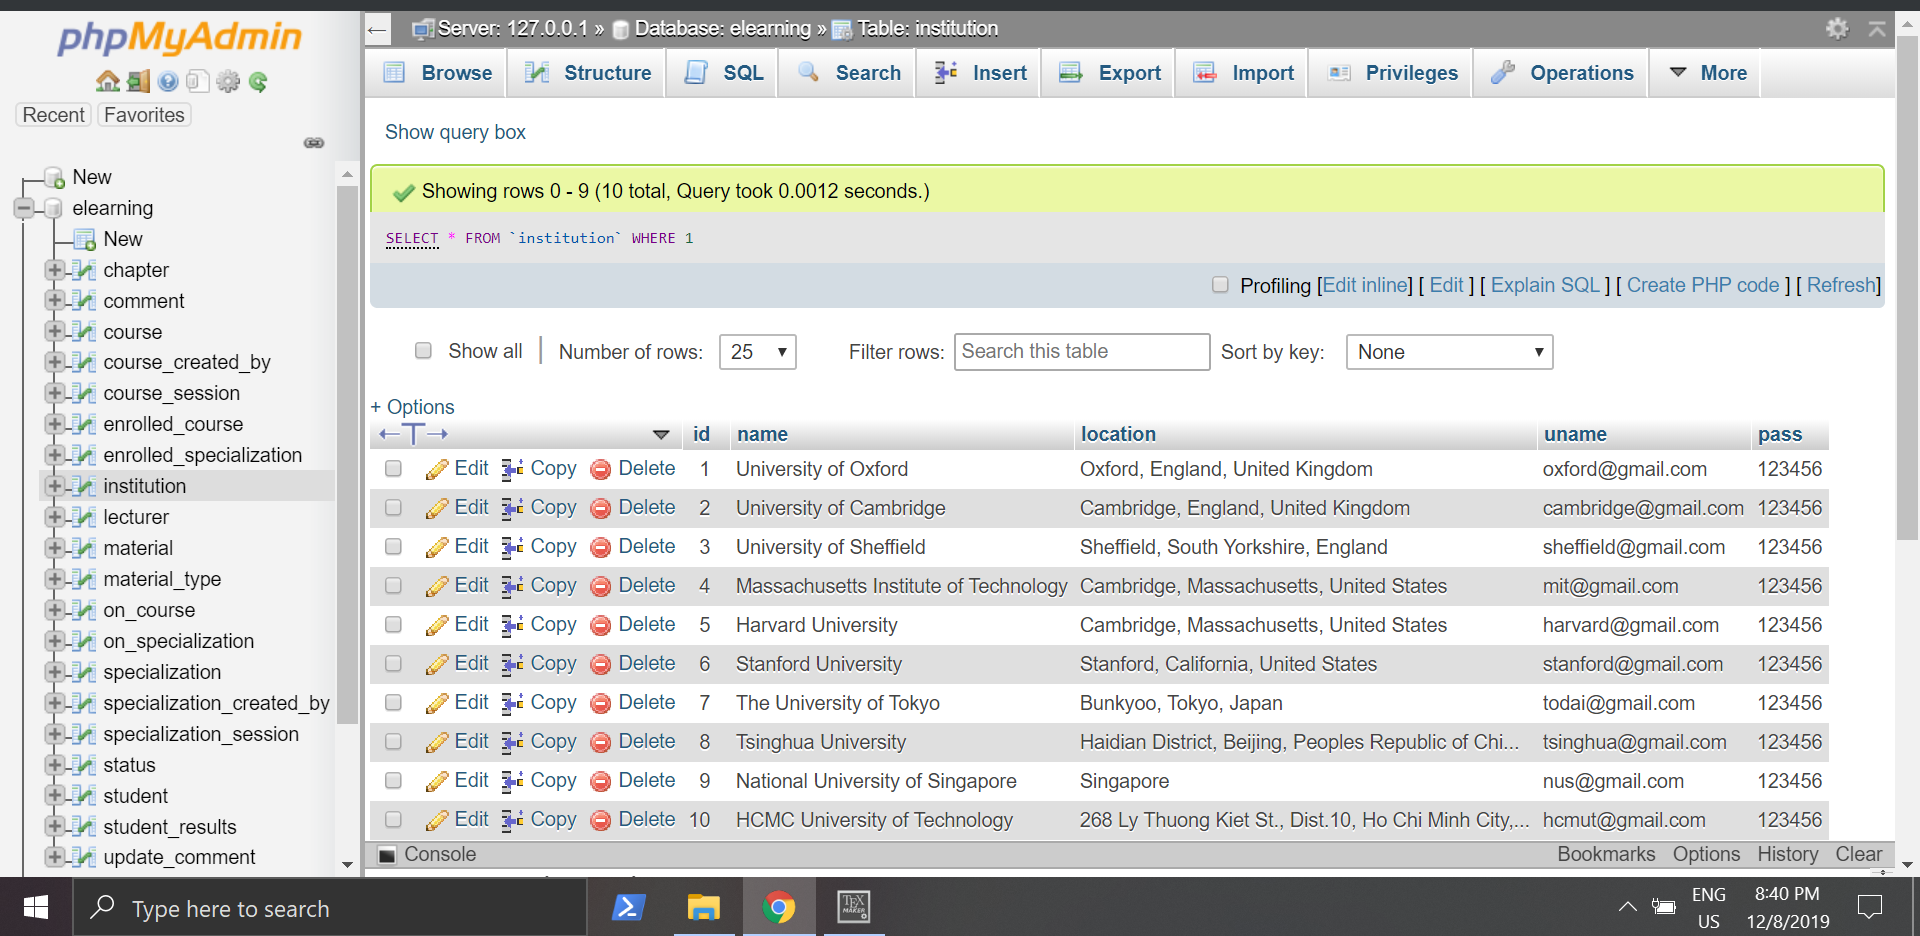
\includegraphics[width=0.8\textwidth]{images/dat8.png}
\end{figure}
\newpage
\begin{figure}[h!]
	\centering
	\caption{Dữ liệu bảng lecturer}
	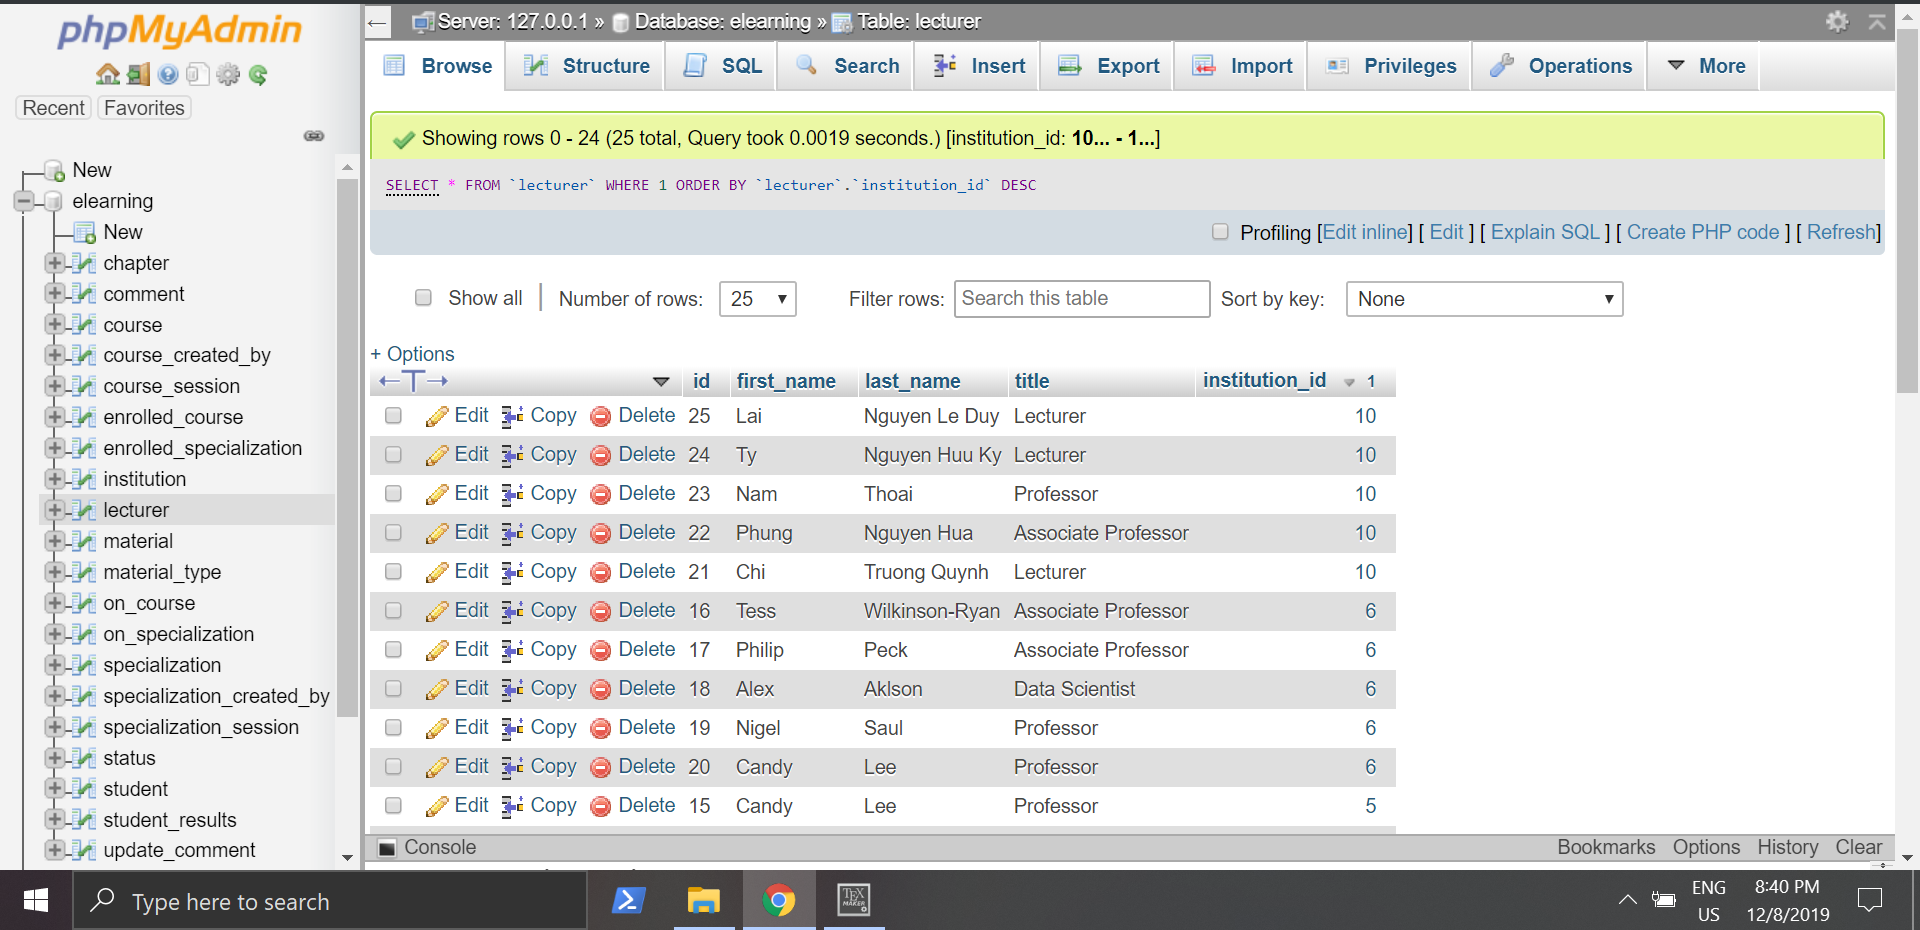
\includegraphics[width=0.8\textwidth]{images/dat9.png}
\end{figure}
\begin{figure}[h!]
	\centering
	\caption{Dữ liệu bảng specialization}
	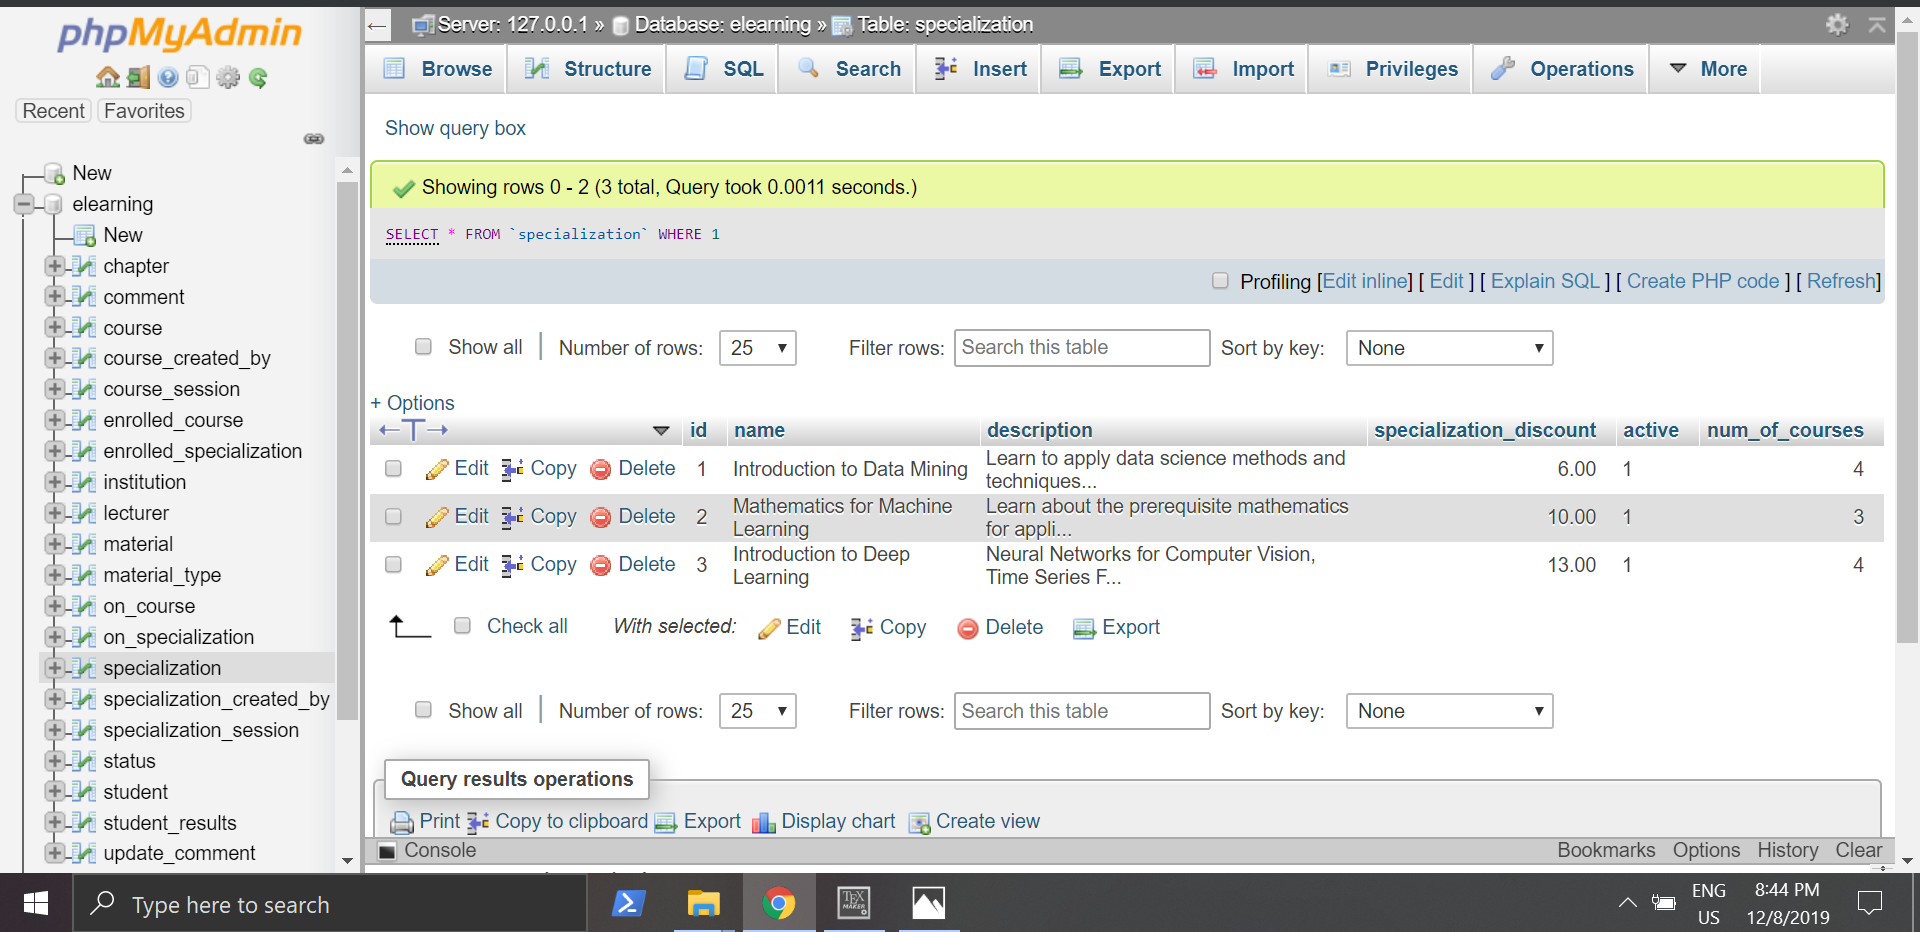
\includegraphics[width=0.8\textwidth]{images/dat14.png}
\end{figure}
\begin{figure}[h!]
	\centering
	\caption{Dữ liệu bảng course}
	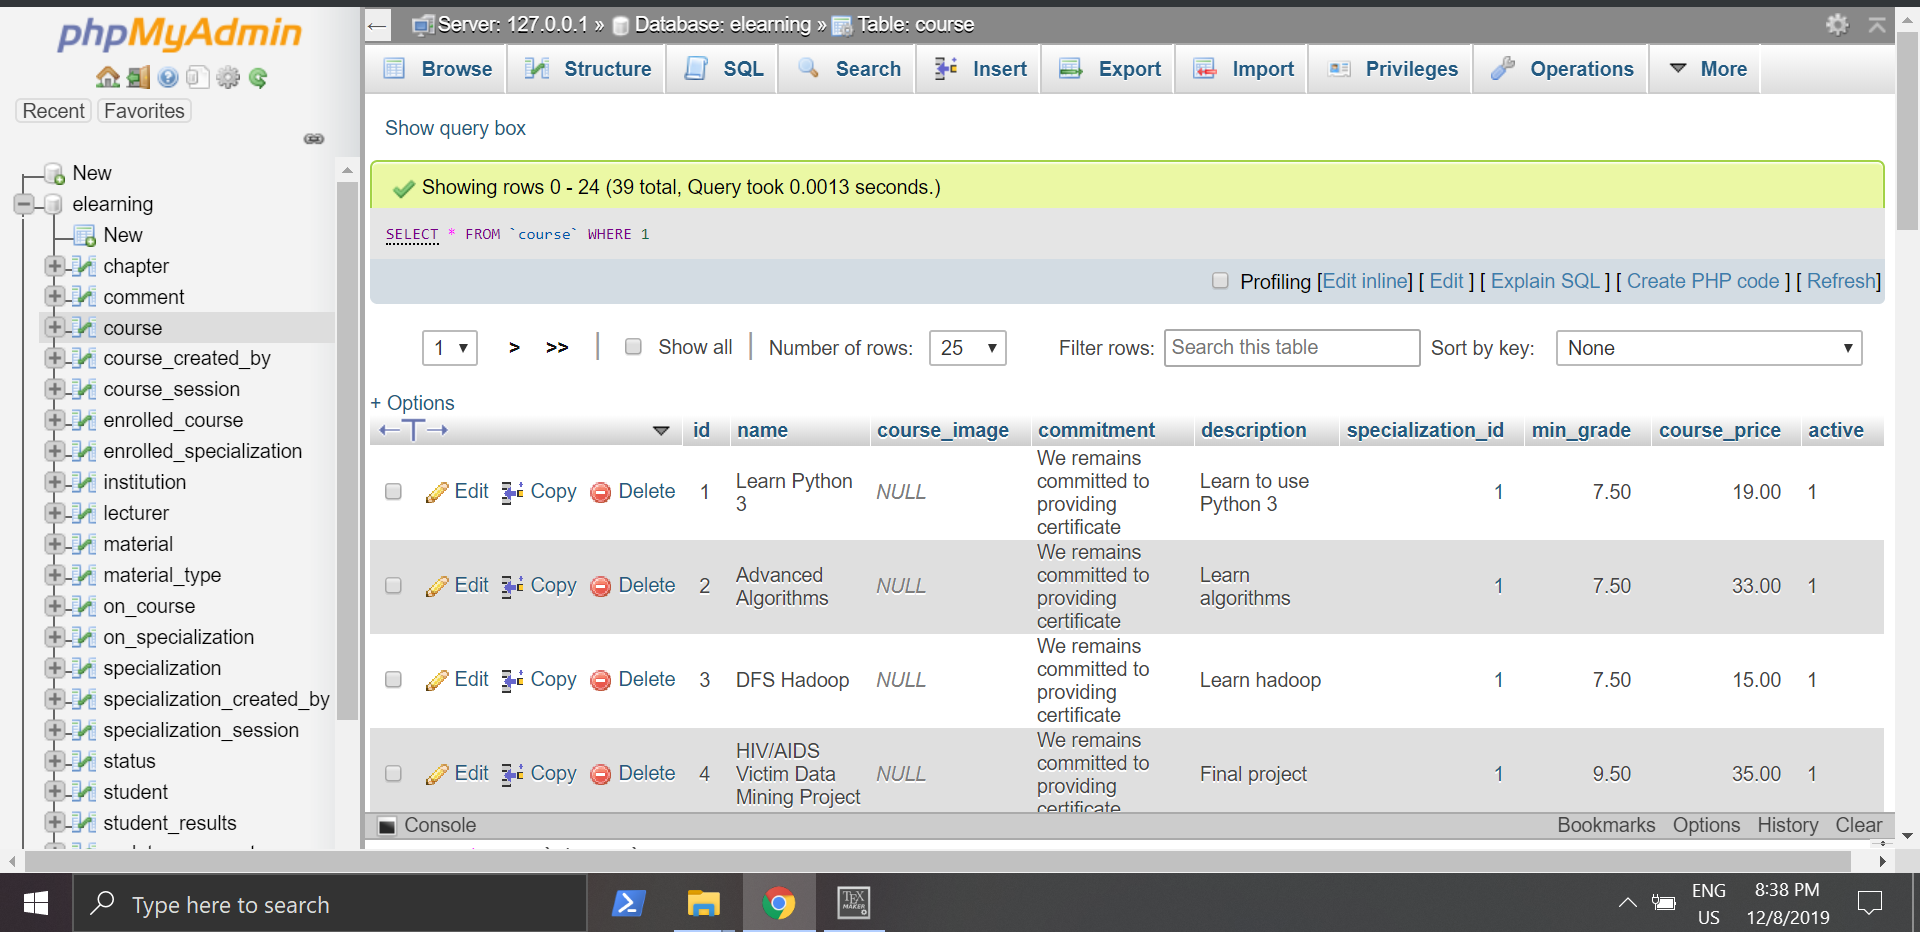
\includegraphics[width=0.8\textwidth]{images/dat2.png}
\end{figure}
\newpage
\begin{figure}[h!]
	\centering
	\caption{Dữ liệu bảng course_created_by}
	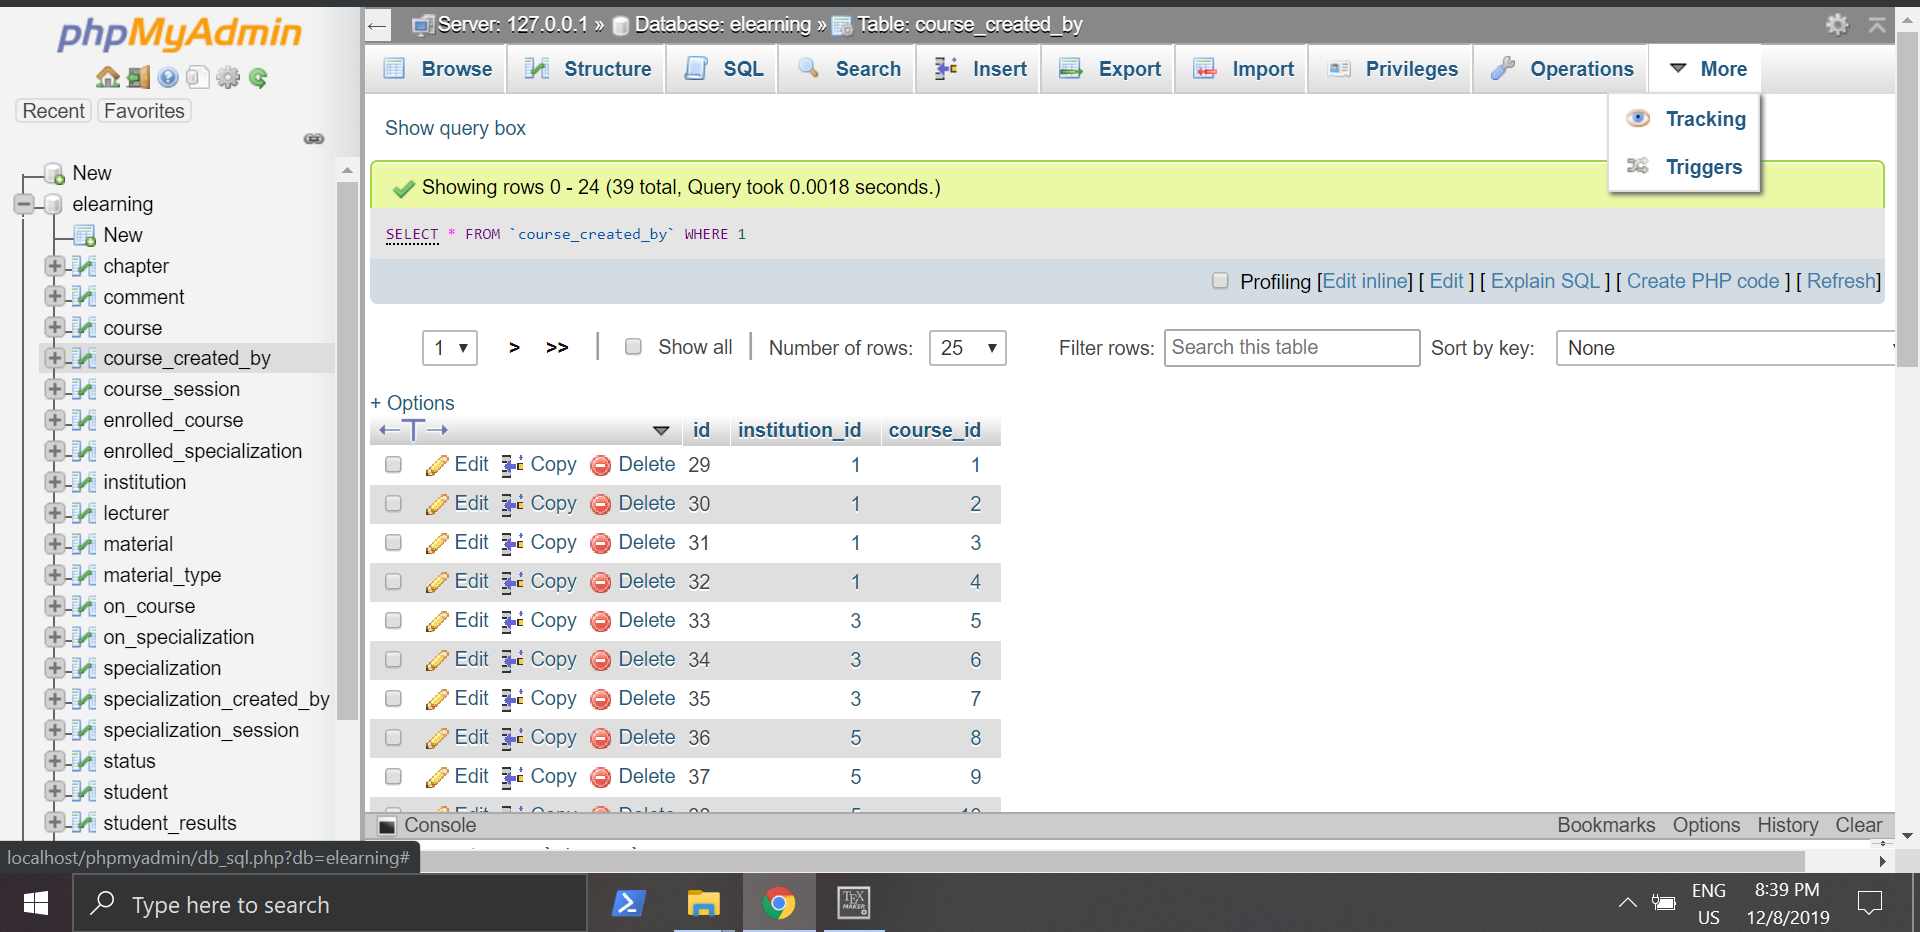
\includegraphics[width=0.8\textwidth]{images/dat4.png}
\end{figure}
\begin{figure}[h!]
	\centering
	\caption{Dữ liệu bảng specialization_created_by}
	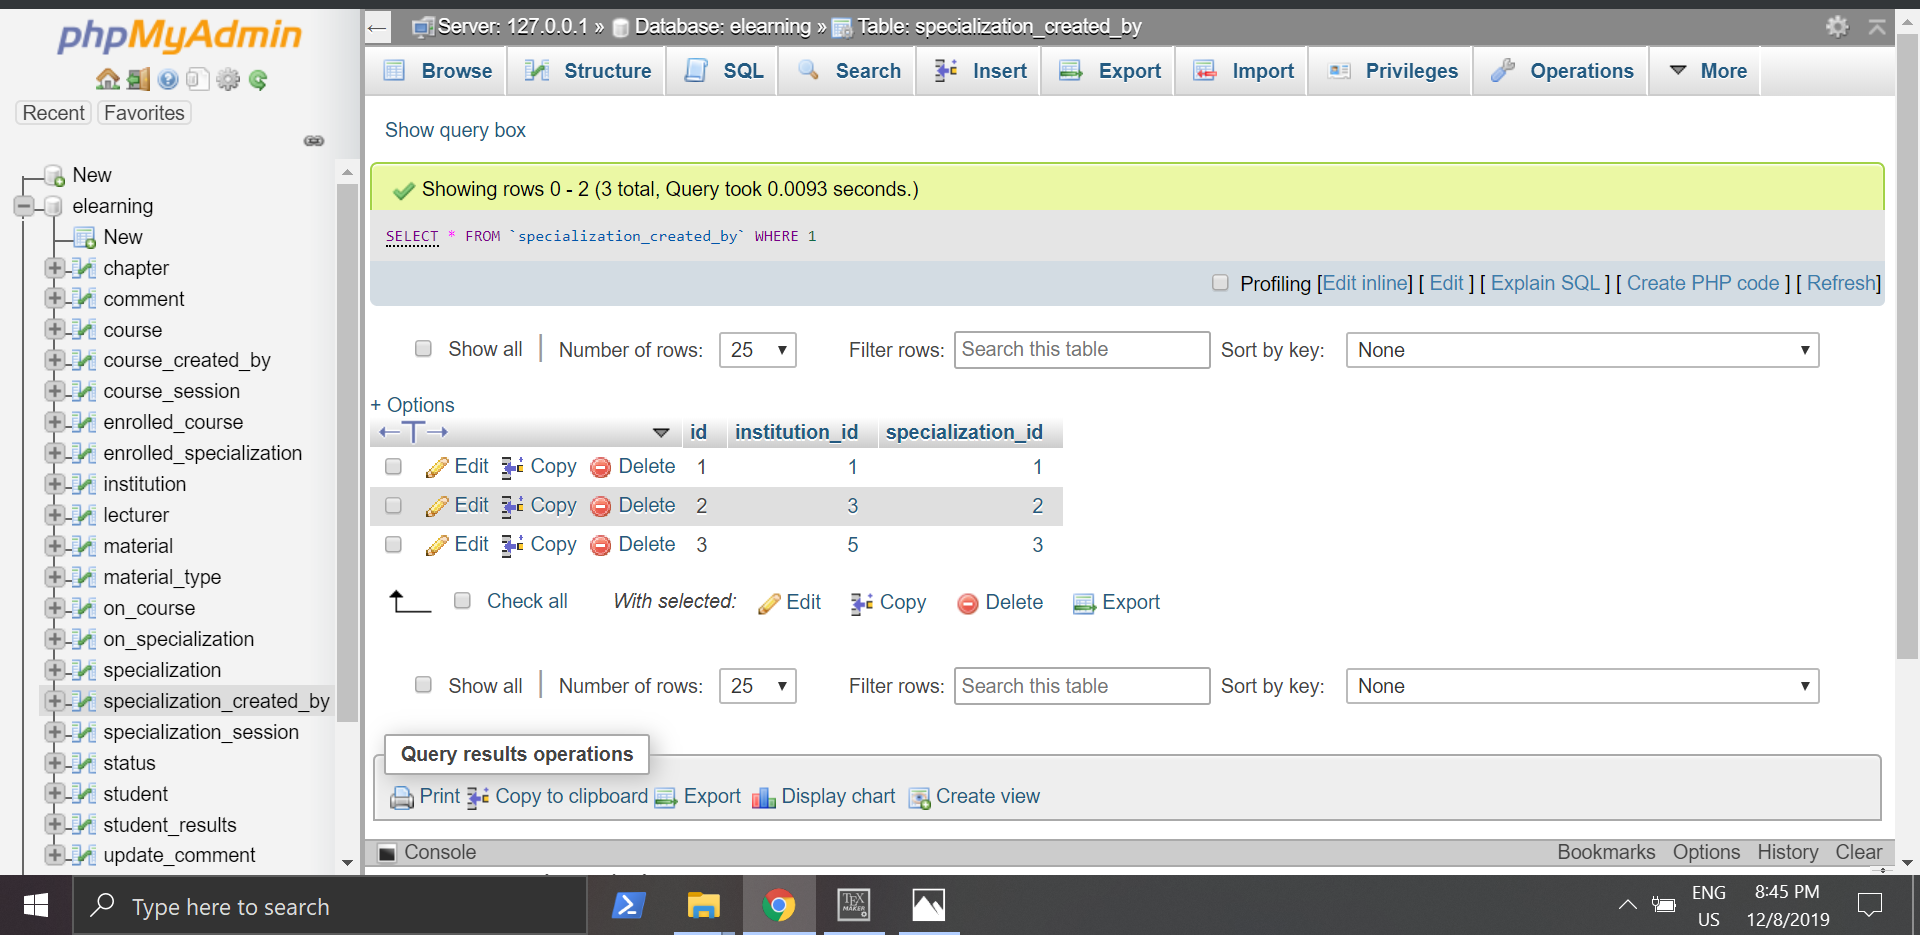
\includegraphics[width=0.8\textwidth]{images/dat15.png}
\end{figure}
\begin{figure}[h!]
	\centering
	\caption{Dữ liệu bảng on_course}
	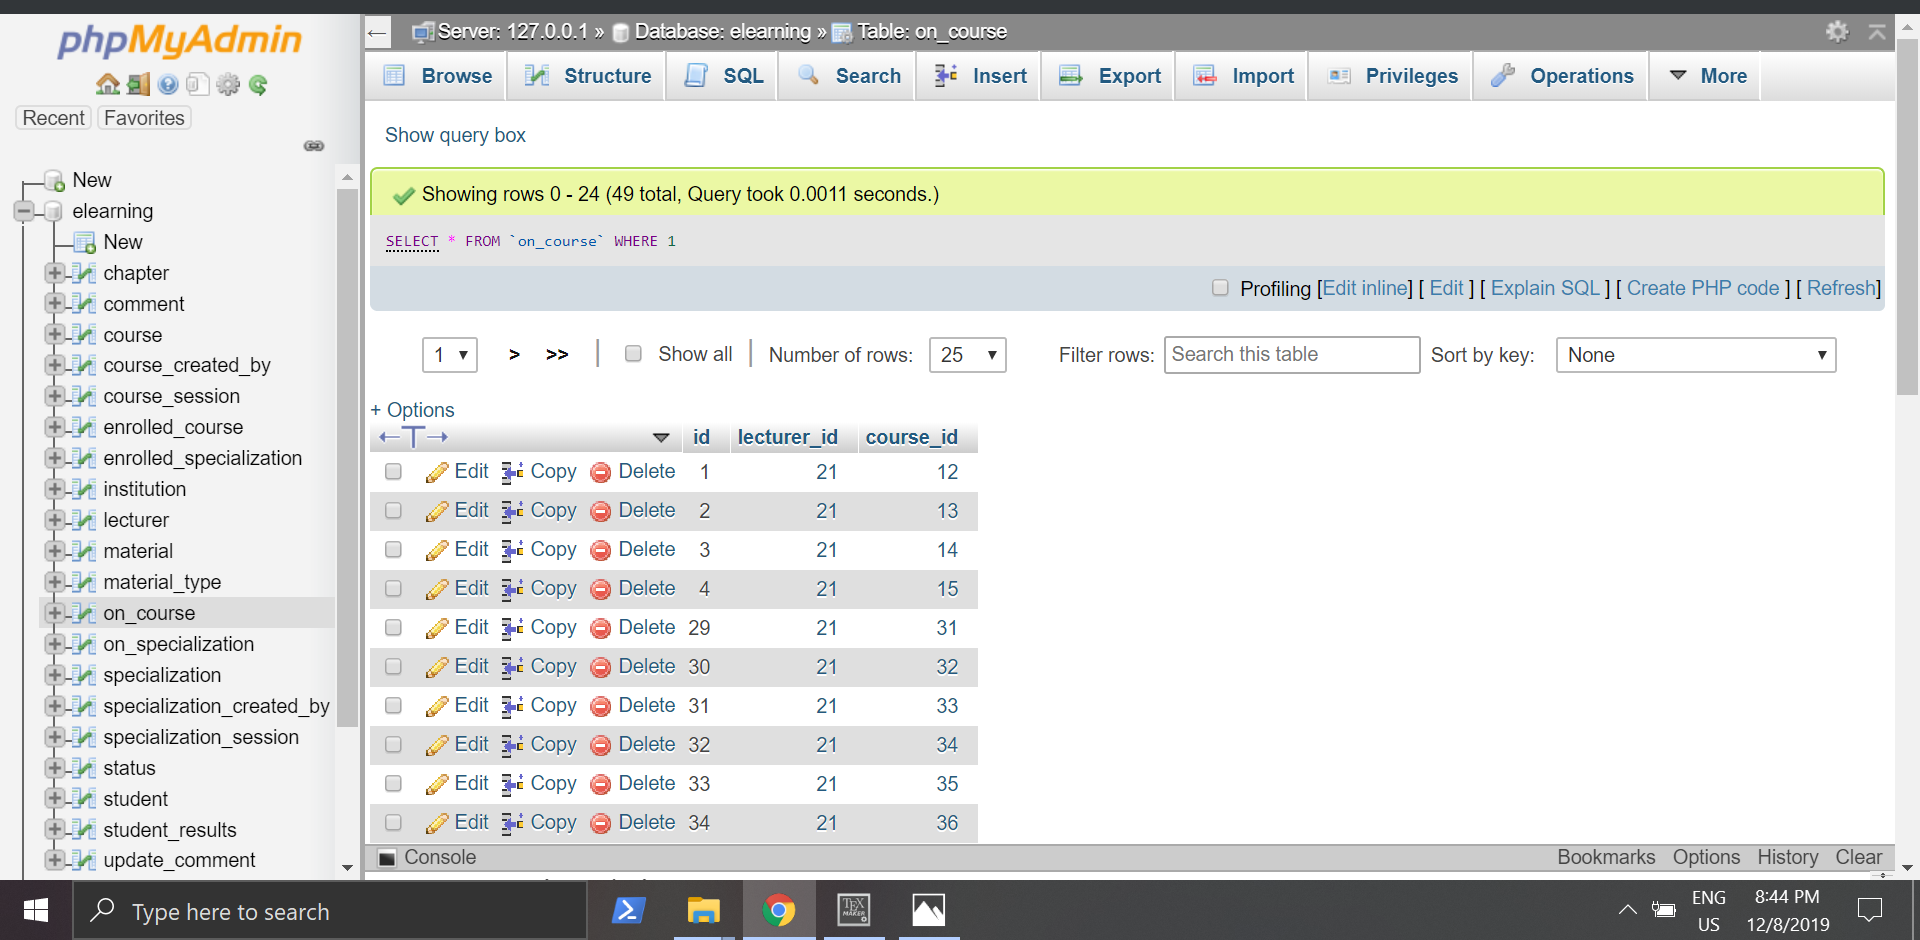
\includegraphics[width=0.8\textwidth]{images/dat12.png}
\end{figure}
\newpage
\begin{figure}[h!]
	\centering
	\caption{Dữ liệu bảng chapter}
	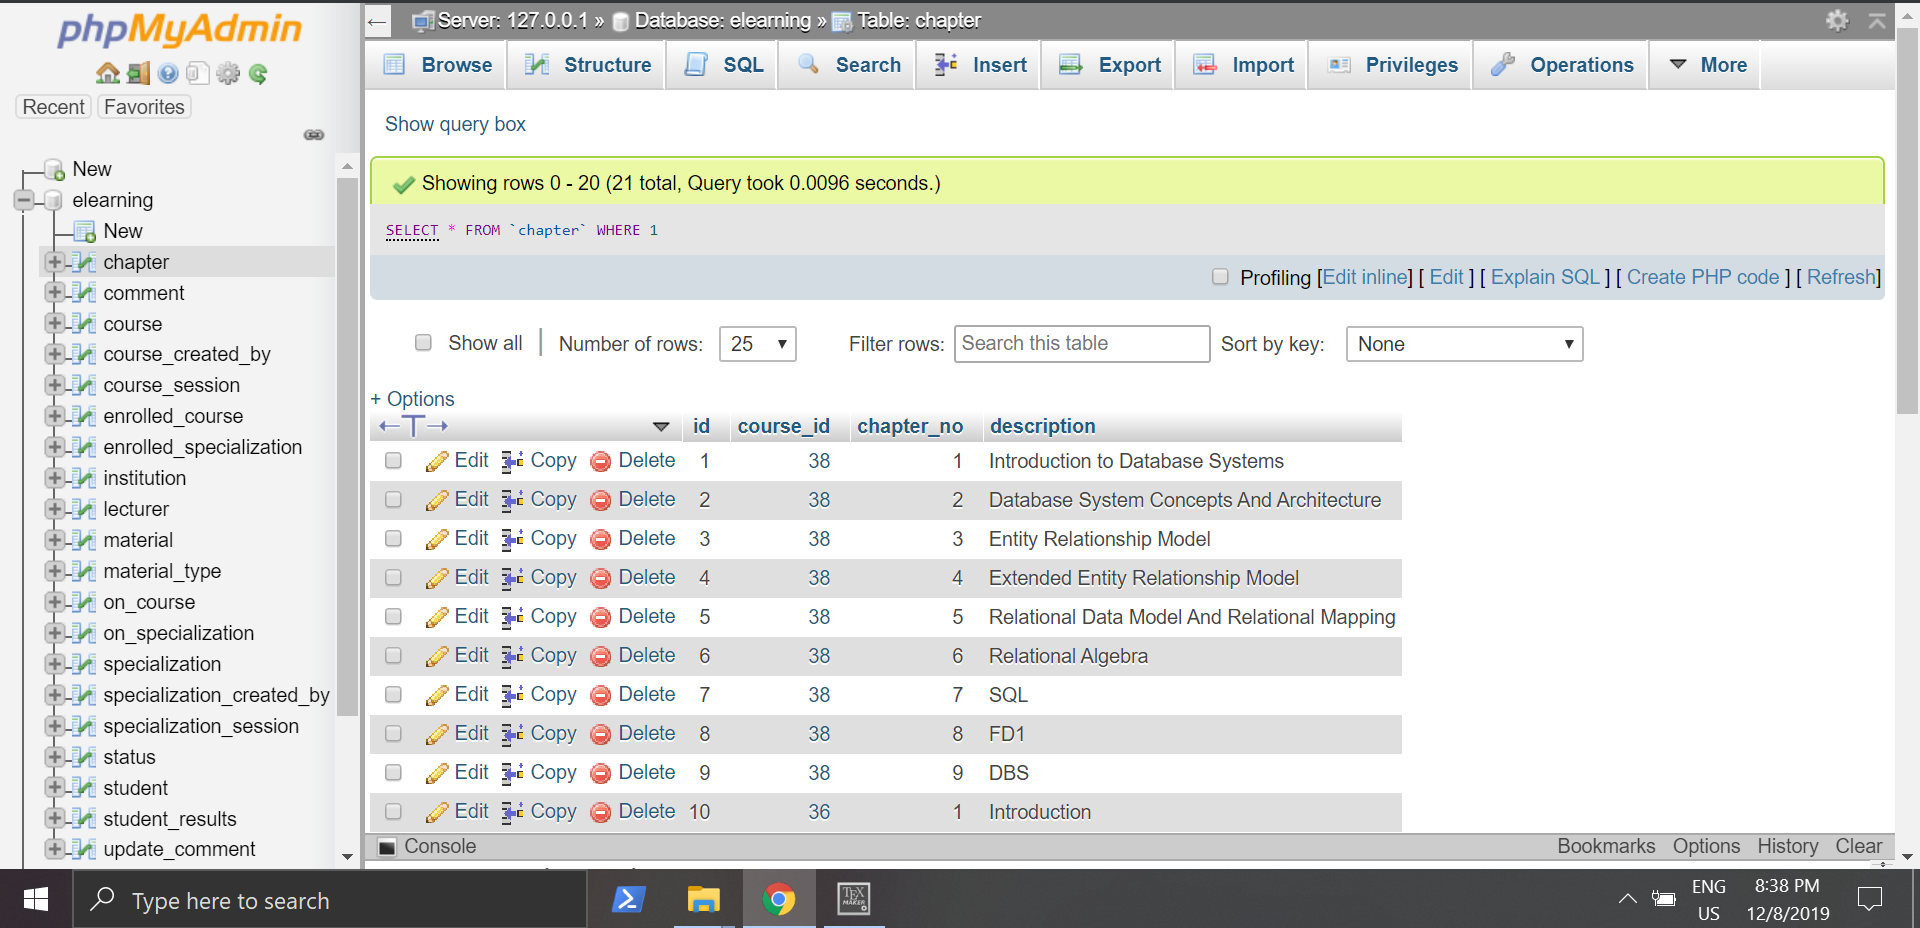
\includegraphics[width=0.8\textwidth]{images/dat1.png}
\end{figure}
\begin{figure}[h!]
	\centering
	\caption{Dữ liệu bảng material_type}
	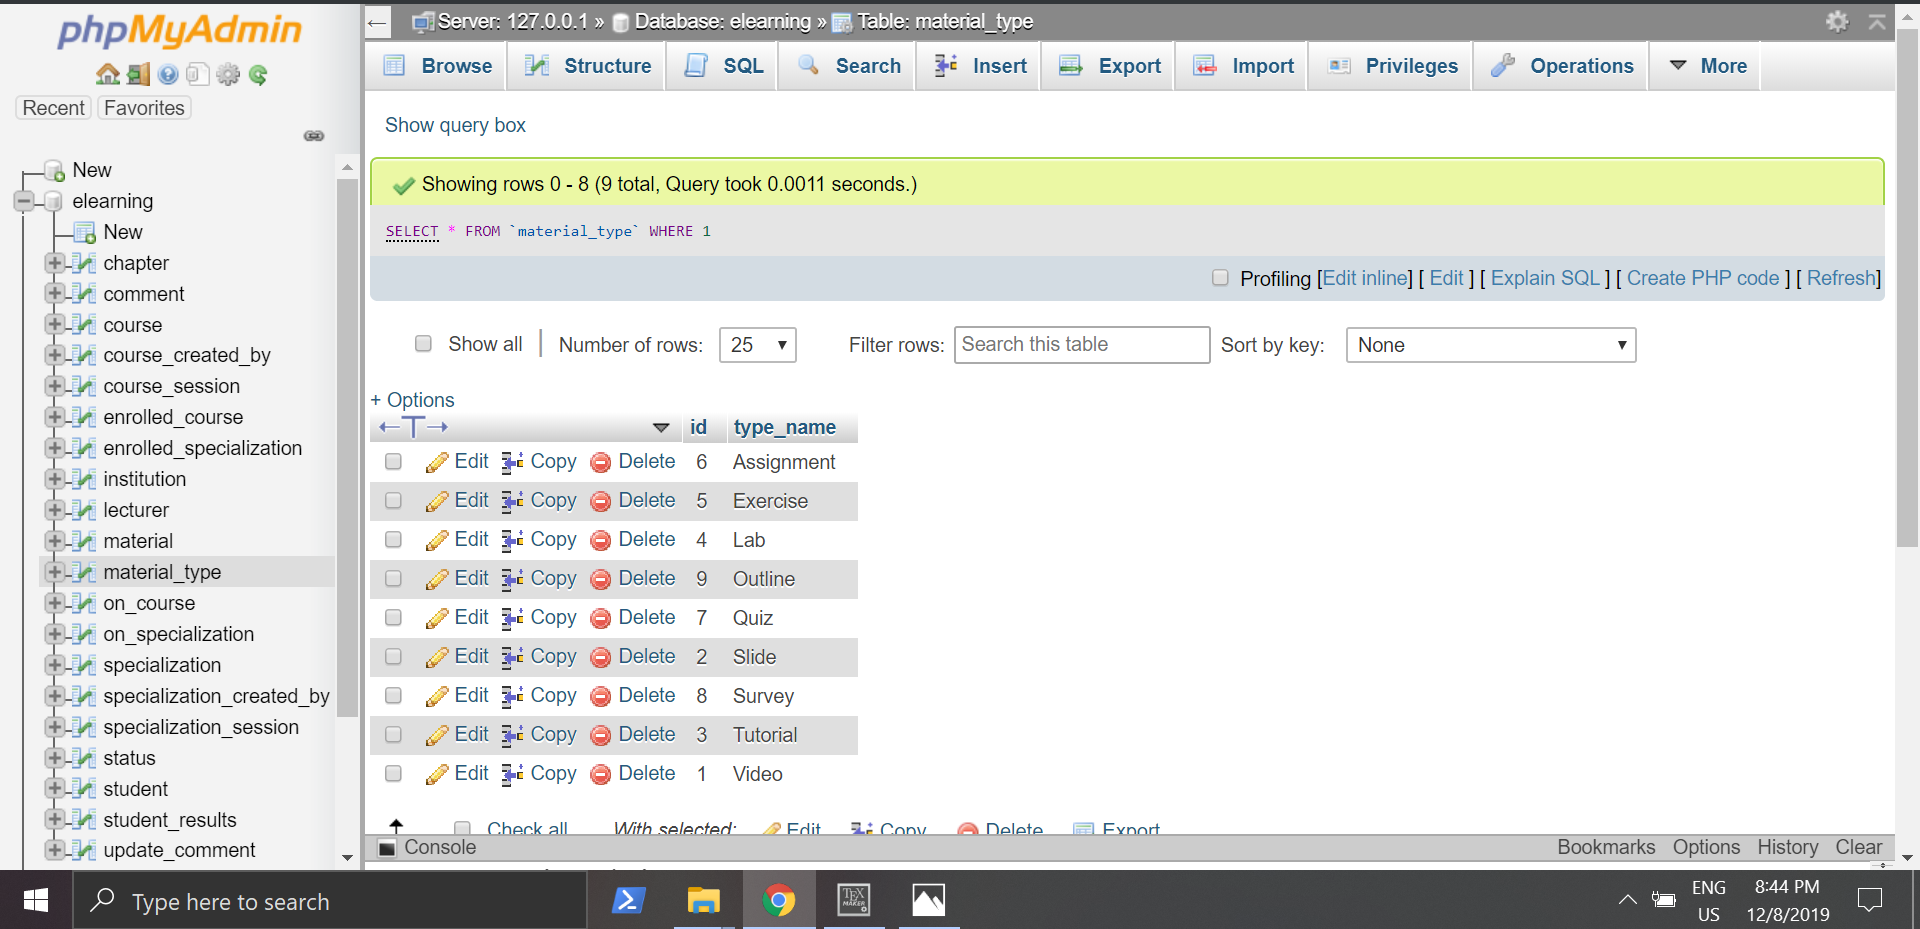
\includegraphics[width=0.8\textwidth]{images/dat11.png}
\end{figure}
\begin{figure}[h!]
	\centering
	\caption{Dữ liệu bảng material}
	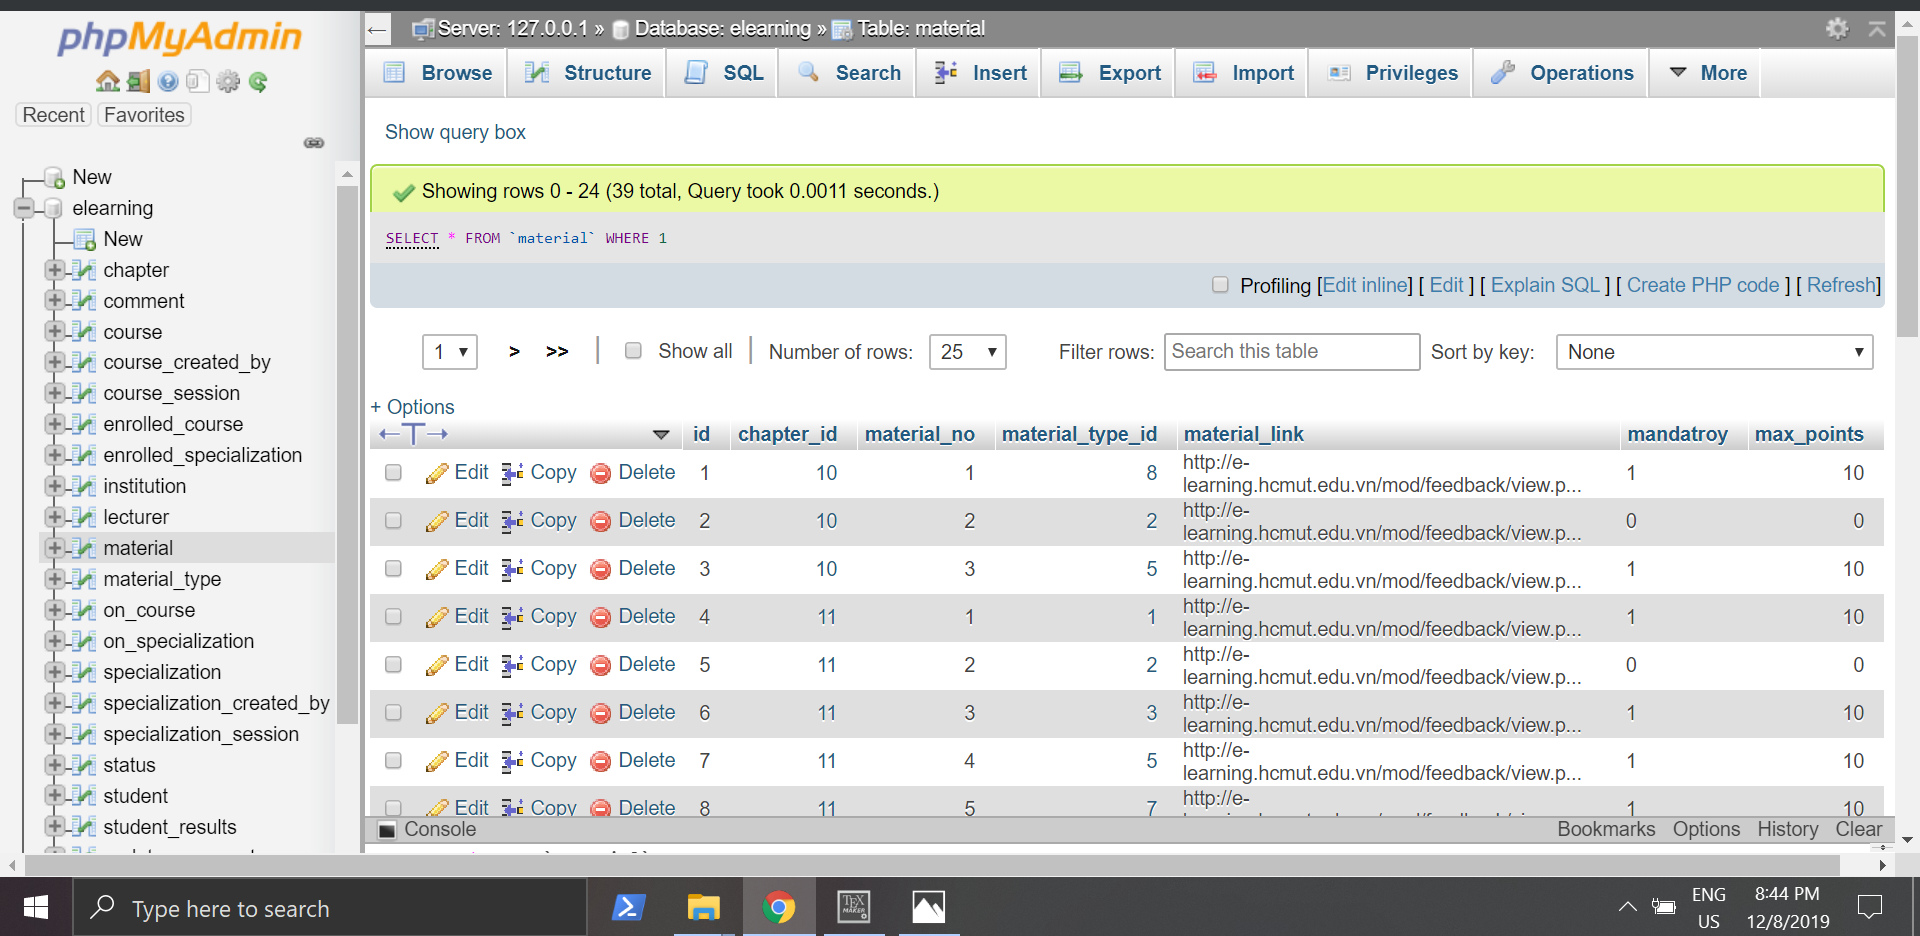
\includegraphics[width=0.8\textwidth]{images/dat10.png}
\end{figure}
\newpage
\begin{figure}[h!]
	\centering
	\caption{Dữ liệu bảng status}
	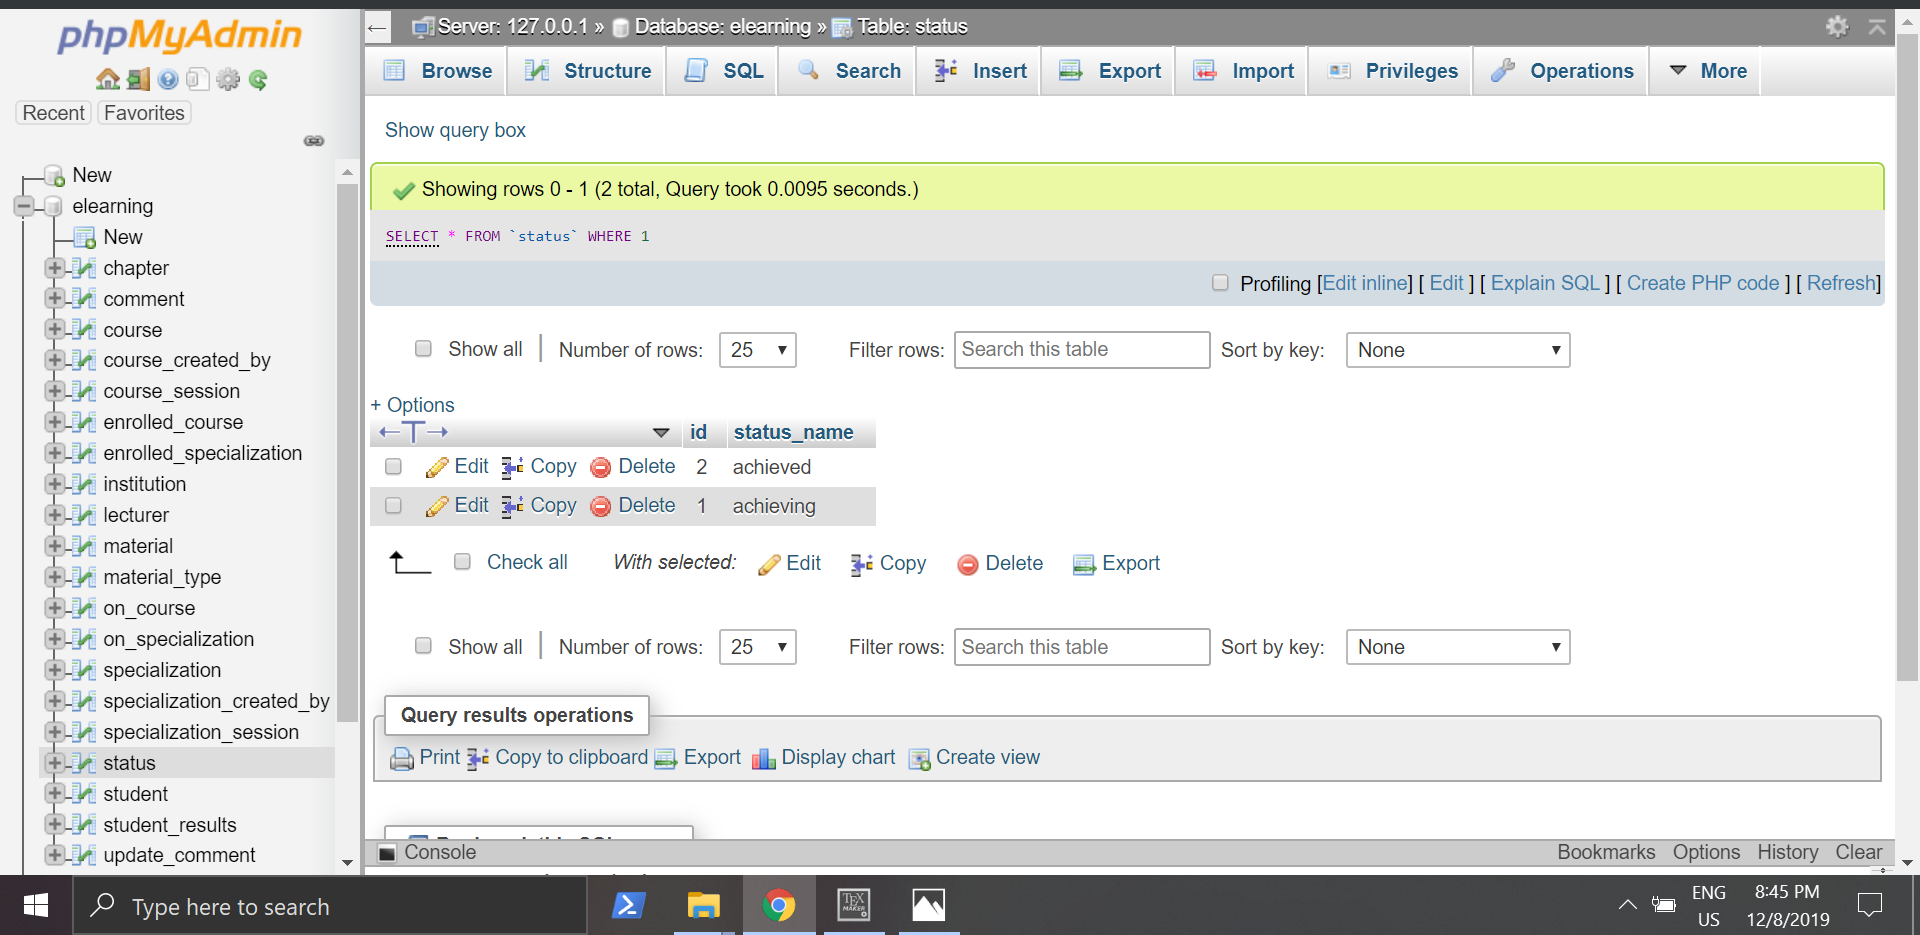
\includegraphics[width=0.8\textwidth]{images/dat17.png}
\end{figure}
\begin{figure}[h!]
	\centering
	\caption{Dữ liệu bảng student}
	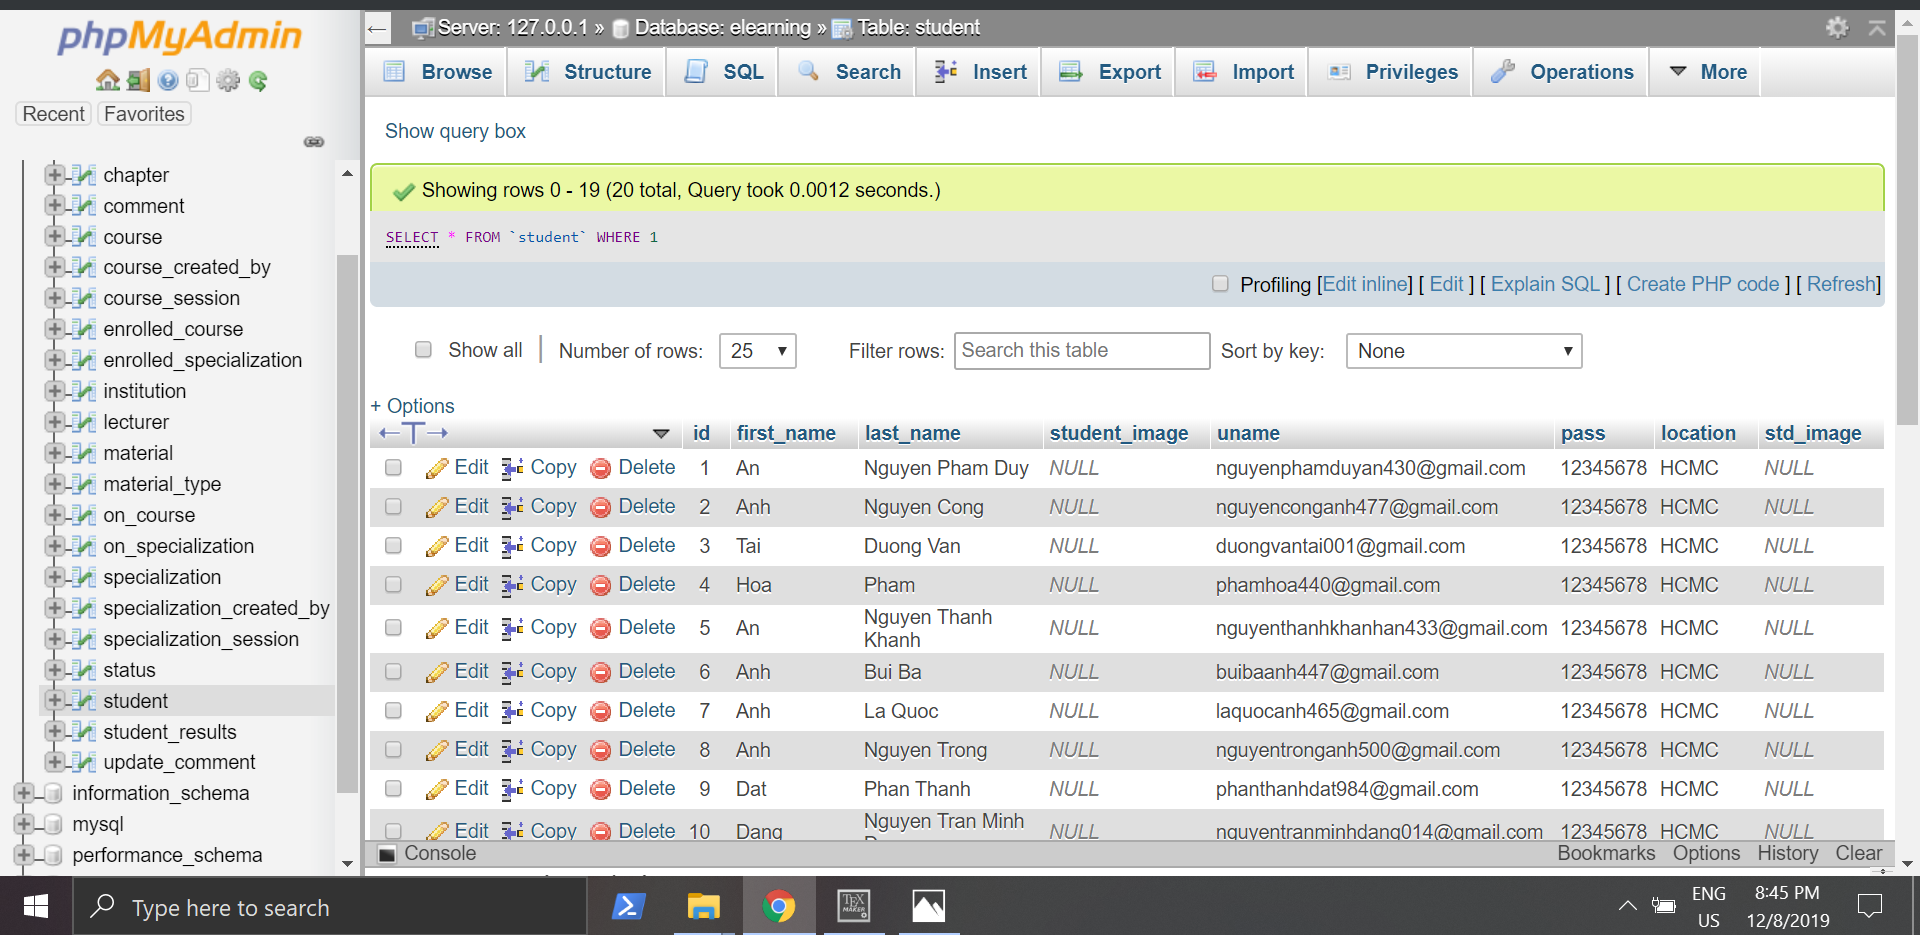
\includegraphics[width=0.8\textwidth]{images/dat18.png}
\end{figure}
\begin{figure}[h!]
	\centering
	\caption{Dữ liệu bảng course_session}
	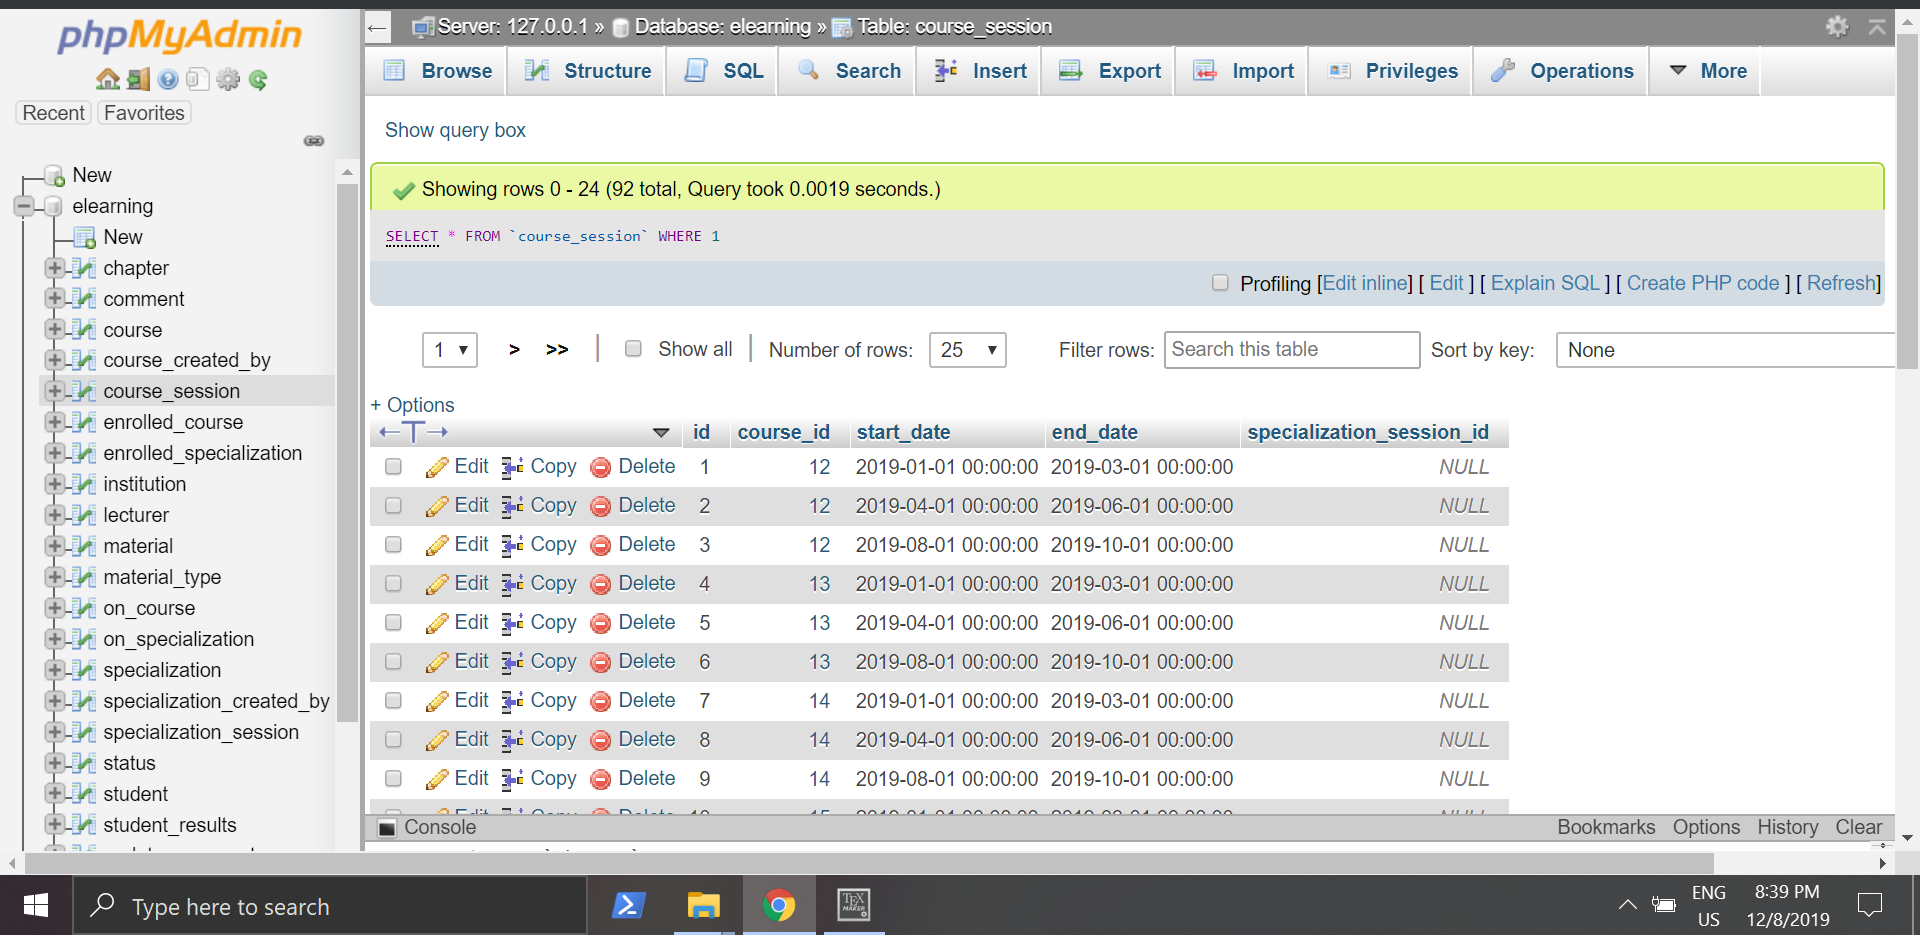
\includegraphics[width=0.8\textwidth]{images/dat5.png}
\end{figure}
\newpage
\begin{figure}[h!]
	\centering
	\caption{Dữ liệu bảng specialization_session}
	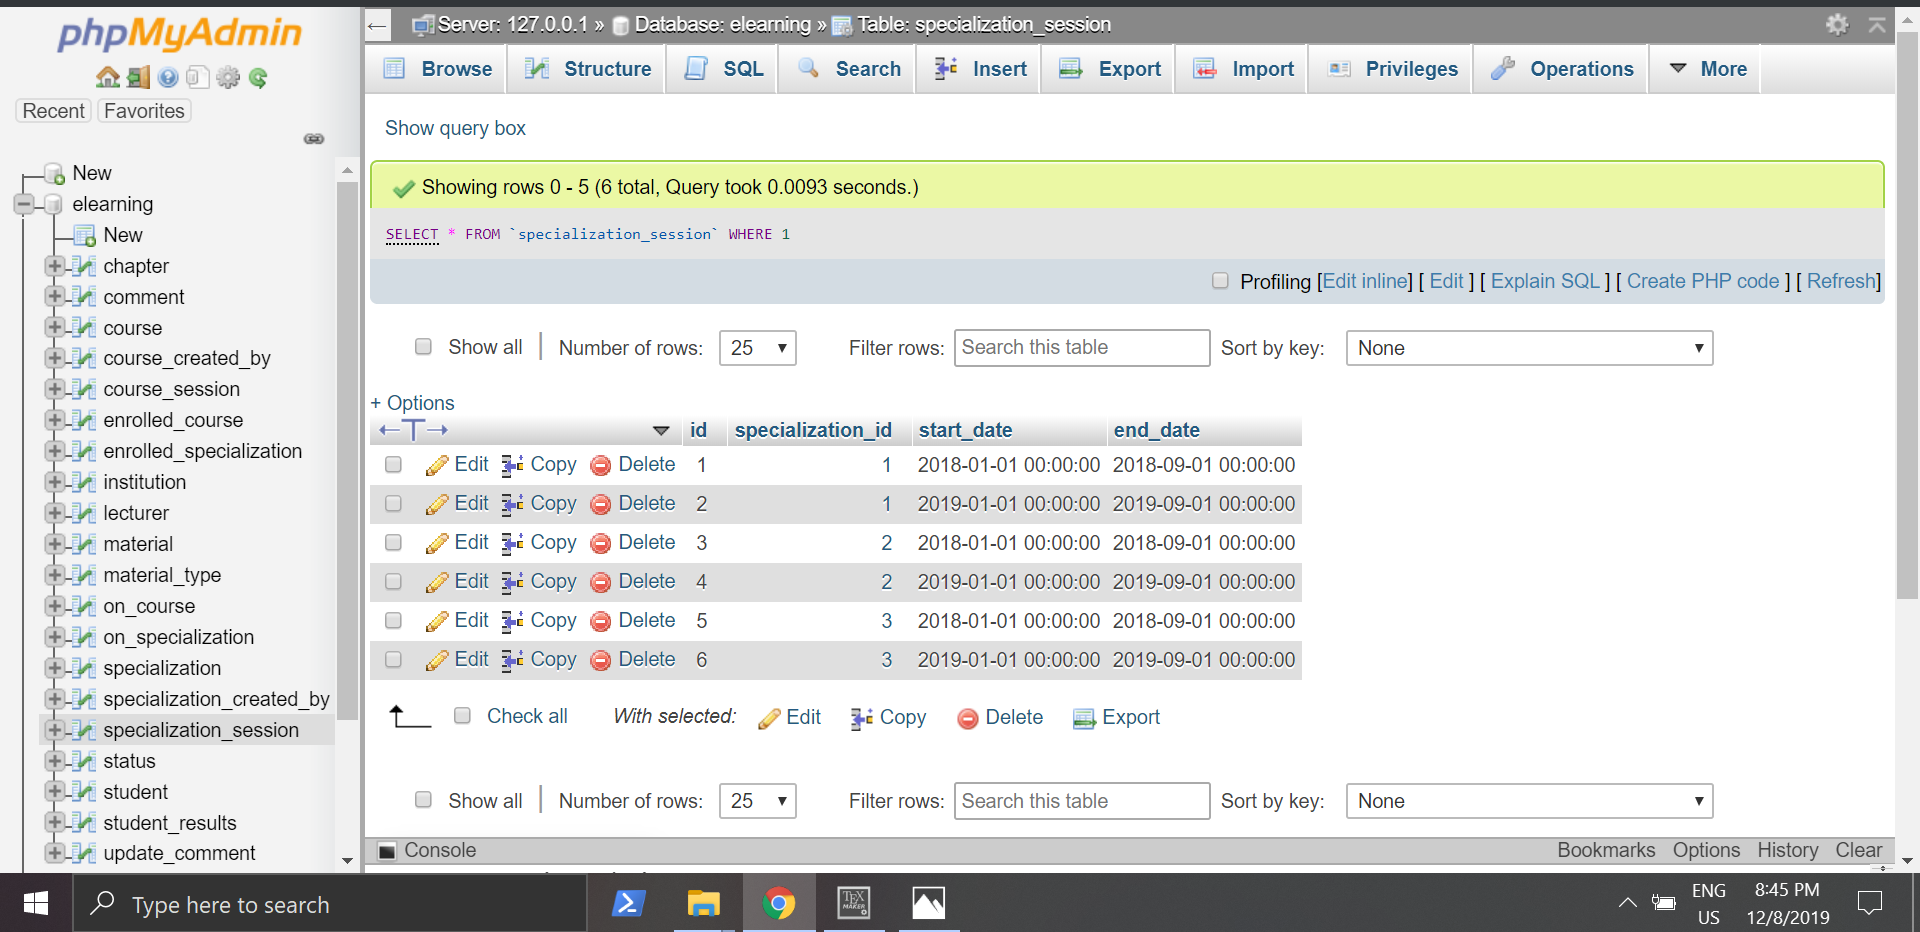
\includegraphics[width=0.8\textwidth]{images/dat16.png}
\end{figure}
\begin{figure}[h!]
	\centering
	\caption{Dữ liệu bảng enrolled_course}
	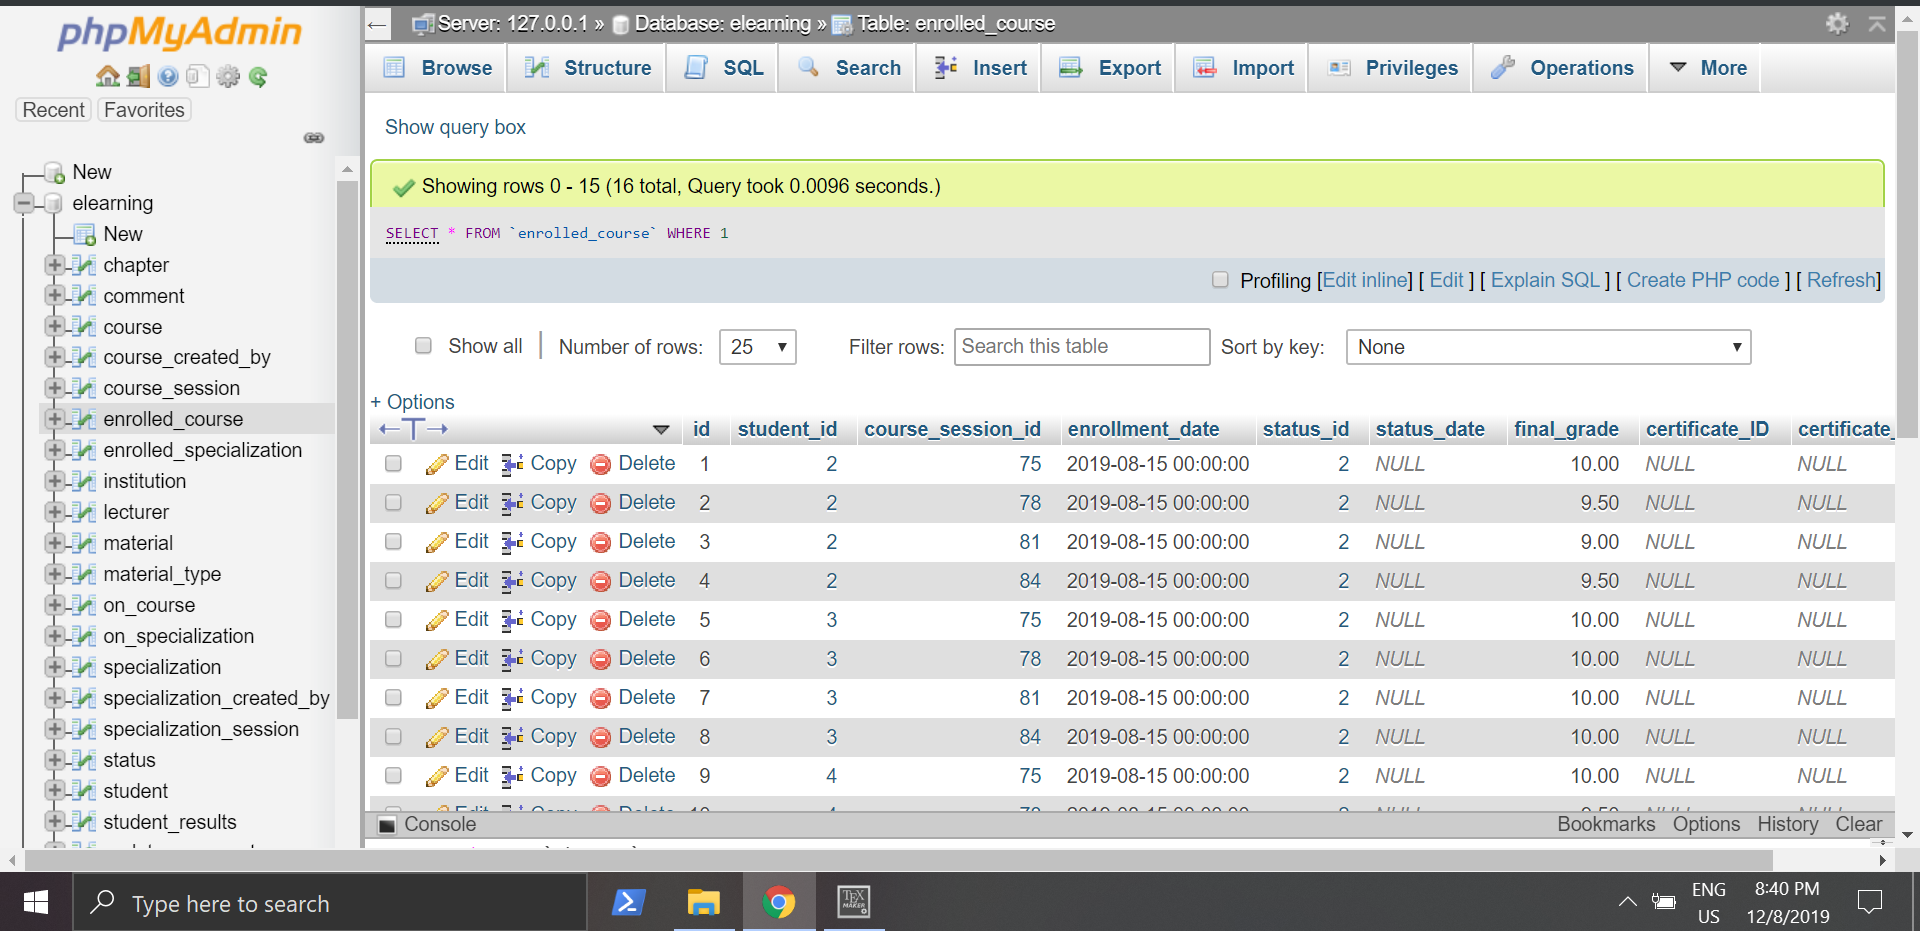
\includegraphics[width=0.8\textwidth]{images/dat6.png}
\end{figure}
\begin{figure}[h!]
	\centering
	\caption{Dữ liệu bảng enrolled_specialization}
	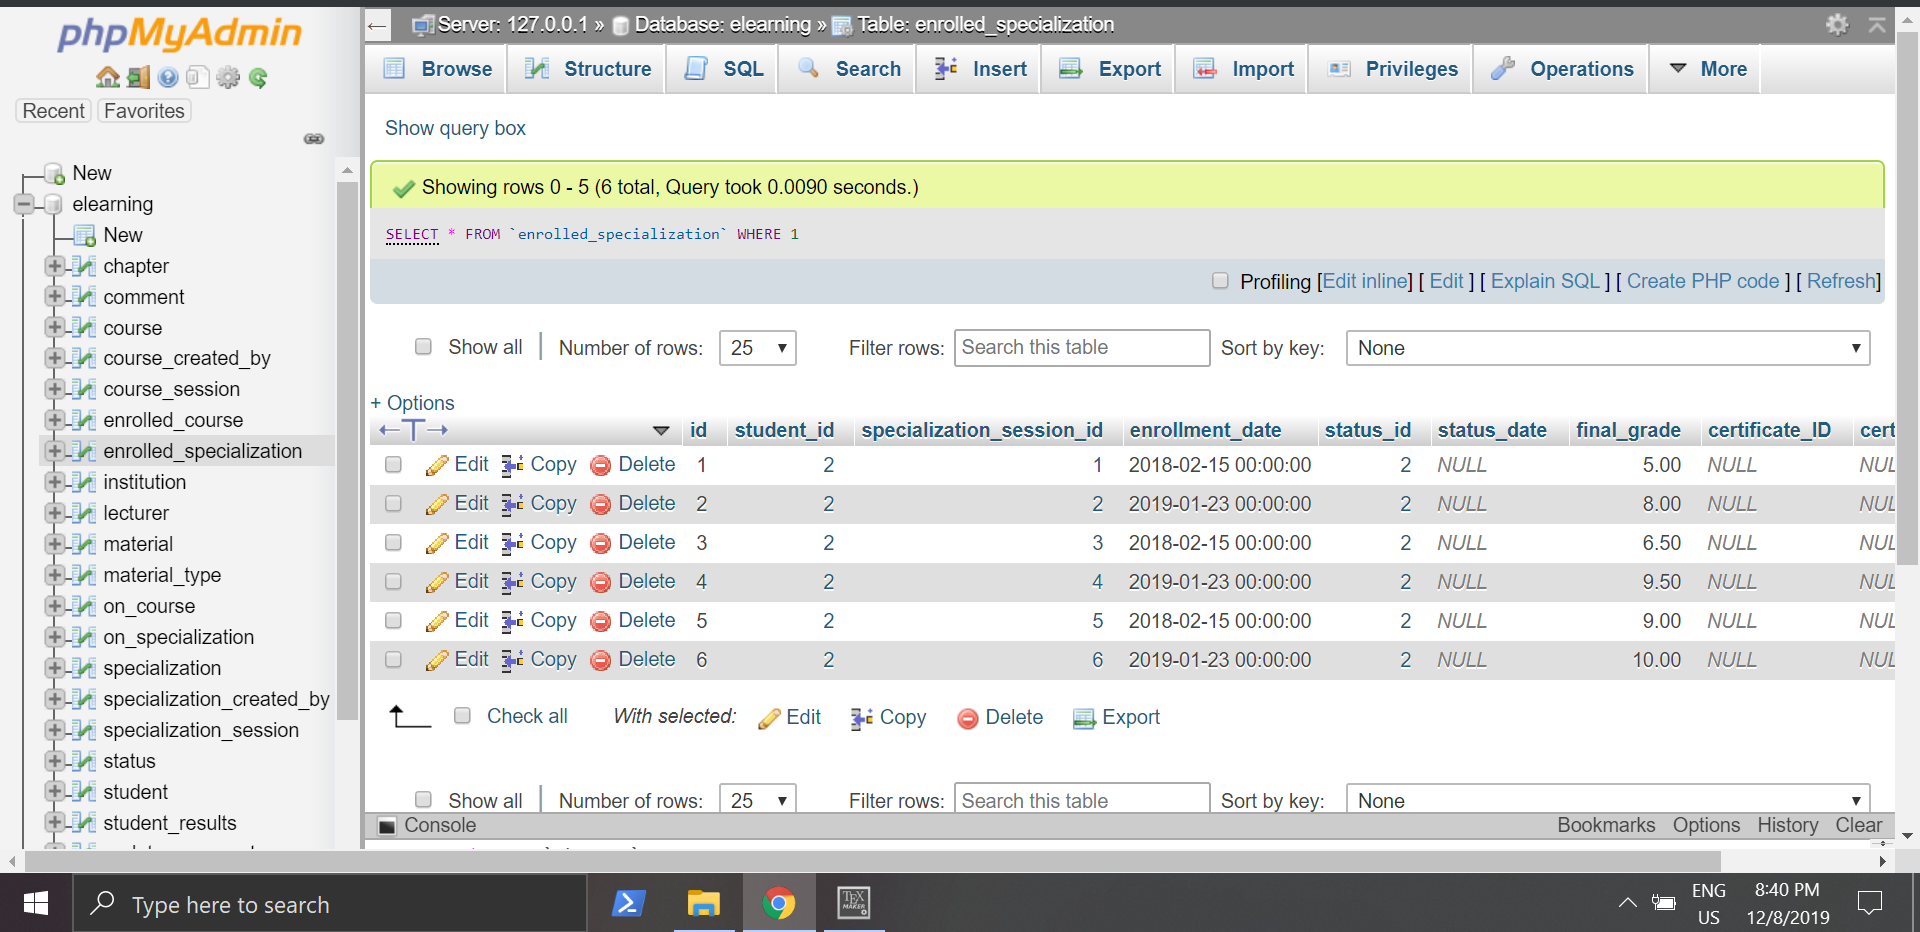
\includegraphics[width=0.8\textwidth]{images/dat7.png}
\end{figure}
\newpage
\begin{figure}[h!]
	\centering
	\caption{Dữ liệu bảng comment}
	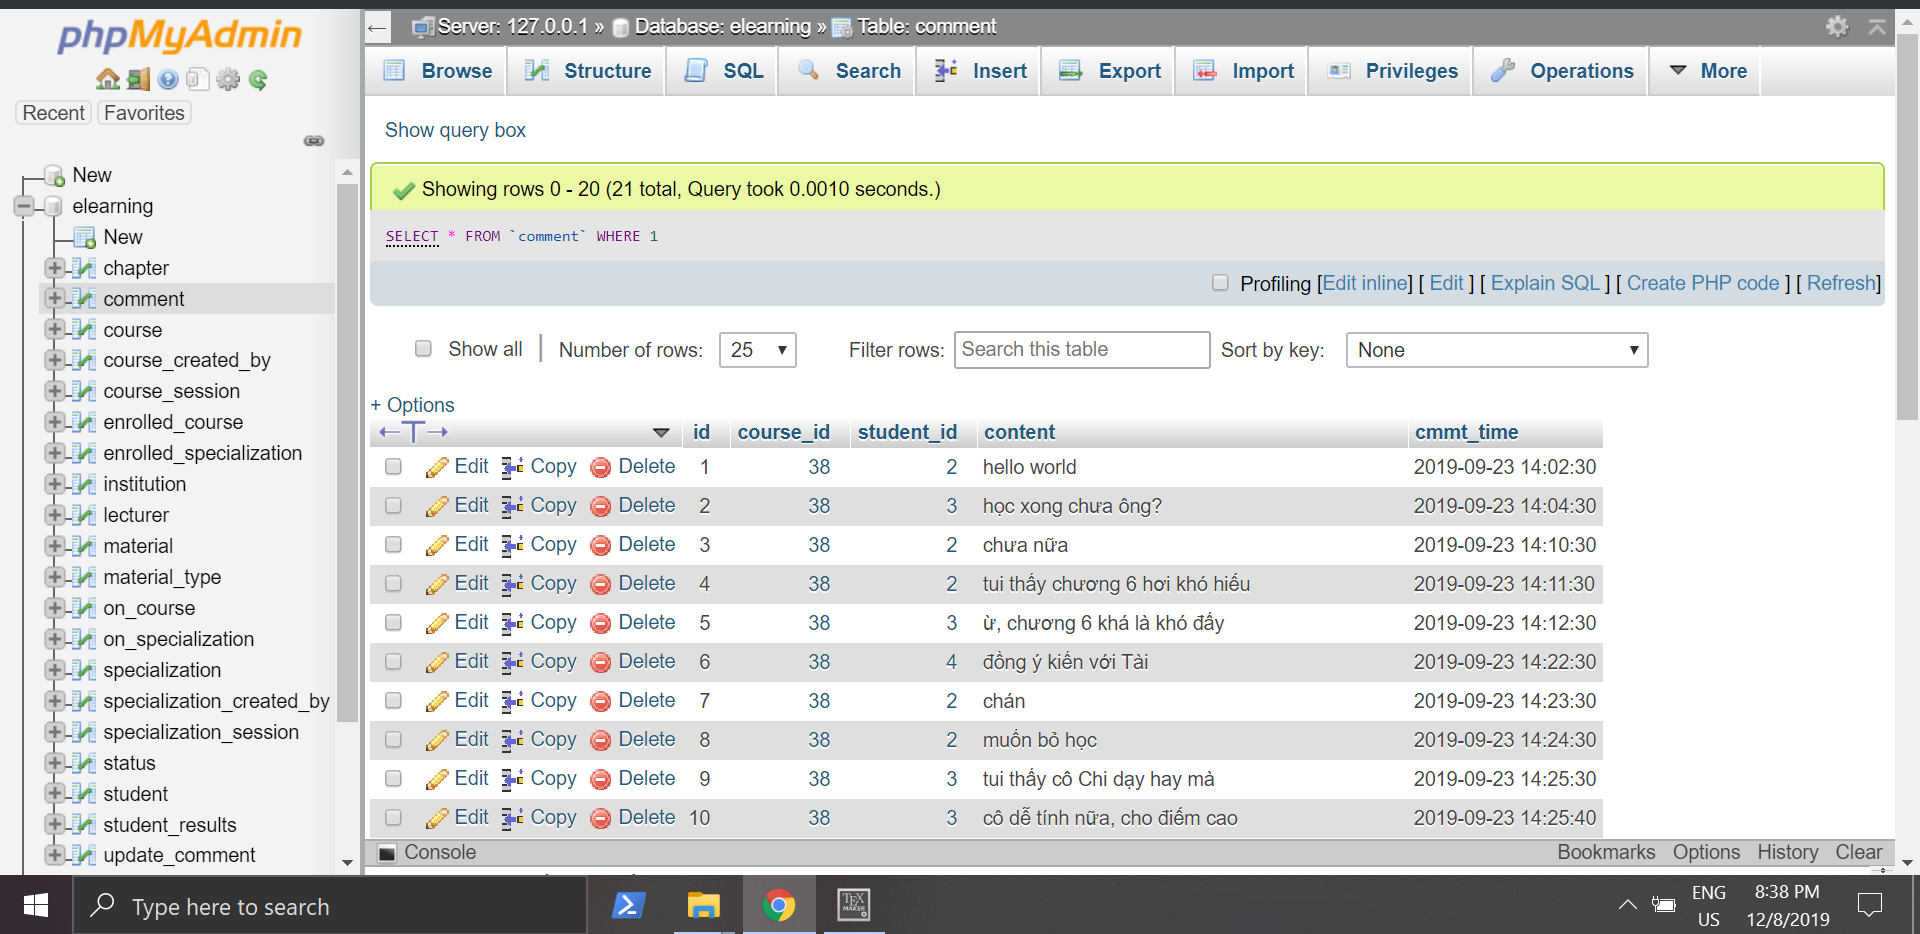
\includegraphics[width=0.8\textwidth]{images/dat3.png}
\end{figure}
\begin{figure}[h!]
	\centering
	\caption{Dữ liệu bảng update_comment}
	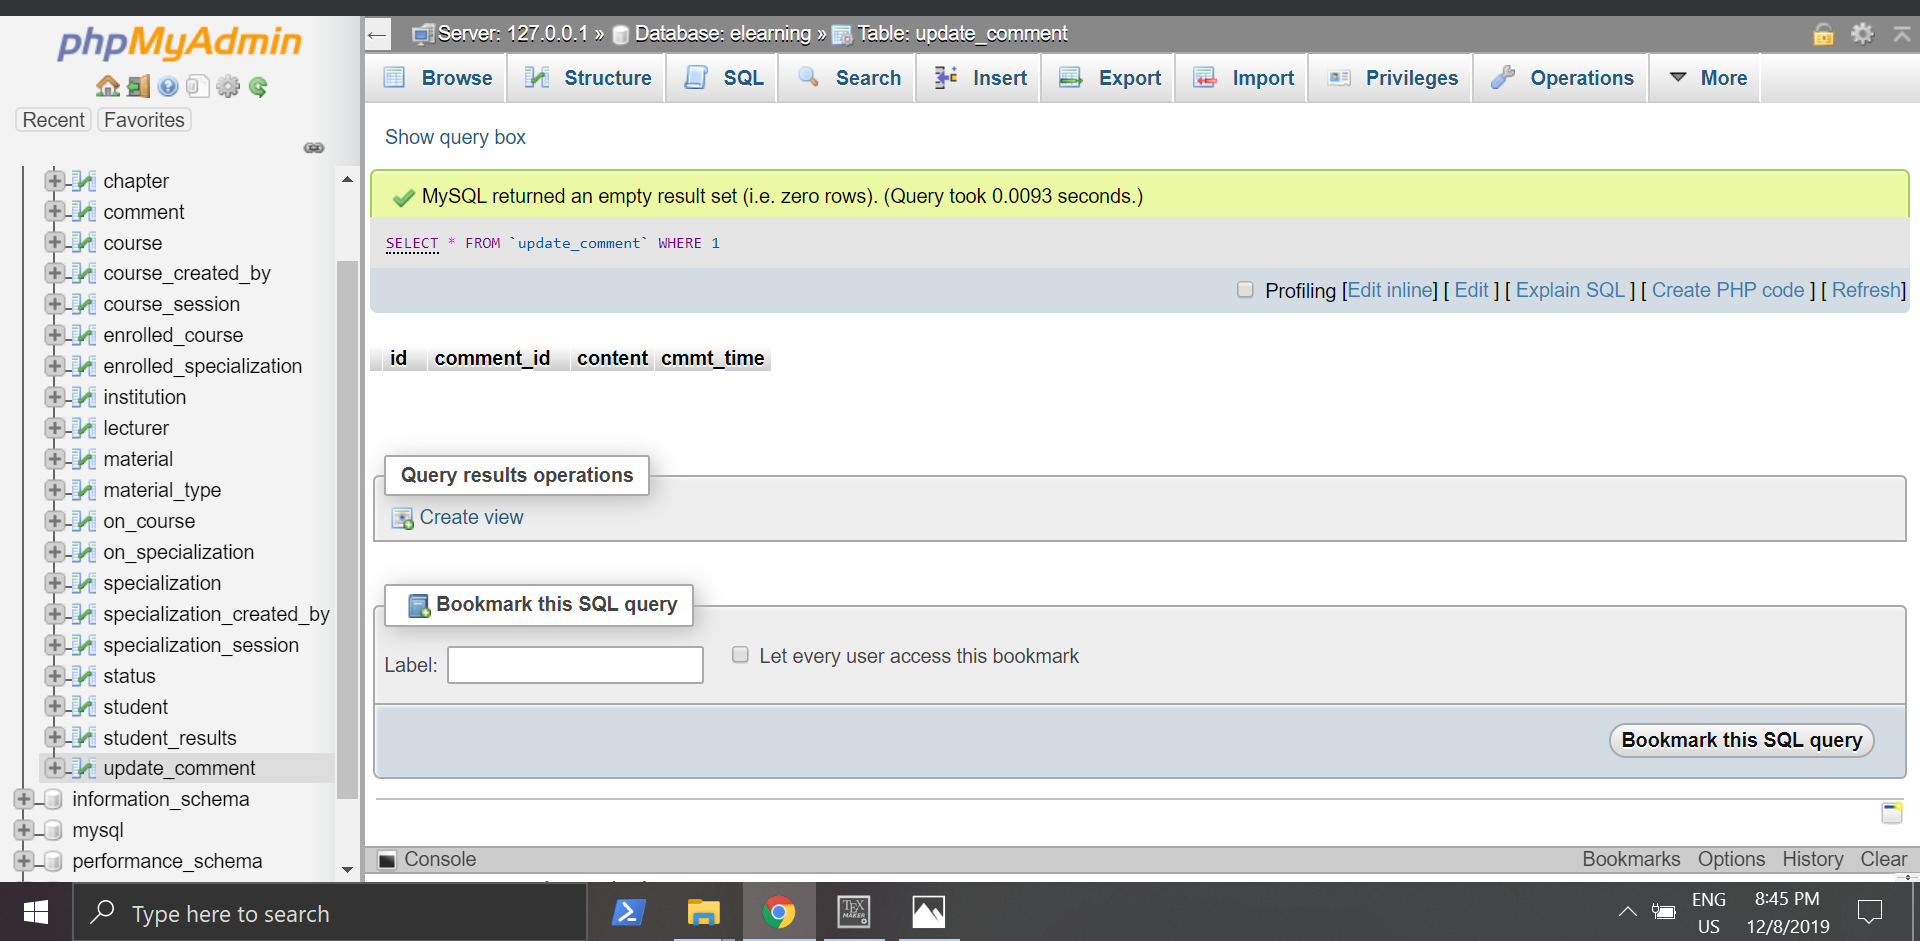
\includegraphics[width=0.8\textwidth]{images/dat20.png}
\end{figure}
\newpage
\section{Phần riêng}
\subsection{Thao tác với bảng dữ liệu course}
\textit{Thành viên 1: Nguyễn Công Anh, MSSV: 1710477}
\subsubsection{Thủ tục Insert dữ liệu}
\textbf{$\bullet$ Mô tả chức năng:} Cho phép insert dữ liệu vào bảng course với inputs là các trường dữ liệu cần nhập. Thân thủ tục sẽ kiểm tra tên khóa học, cam kết, mô tả khóa học,... có phải là NULL hoặc có độ dài là 0 hay không, nếu điều kiện kiểm tra đúng thì sẽ thông báo lỗi. Đối với mã khóa học, nếu người dùng nhập NULL thì sẽ được tăng theo AUTO_INCREMENT, còn nếu nhập mã cụ thể thì sẽ insert mã cụ thể đó.\\
\textbf{$\bullet$ Lệnh tạo thủ tục:}
\begin{lstlisting}
DELIMITER $$
CREATE PROCEDURE create_course
(
	c_id int,
	c_name varchar(255),
	c_image text,
	c_commitment varchar(255),
	c_description text,
	c_specialization_id int,
	c_min_grade decimal(5,2),
	c_price decimal(8,2),
	c_active bit
)
sp: BEGIN
	--
	IF (c_name IS NULL OR LENGTH(c_name) = 0)
	THEN
		SIGNAL SQLSTATE '45000'
		SET MESSAGE_TEXT = 'invalid course name';
		LEAVE sp;
	END IF;
	--
	IF (c_commitment IS NULL OR LENGTH(c_commitment) = 0)
	THEN
		SIGNAL SQLSTATE '45000'
		SET MESSAGE_TEXT = 'invalid course commitment';
		LEAVE sp;
	END IF;
	--
	IF (c_description IS NULL OR LENGTH(c_description) = 0)
	THEN
		SIGNAL SQLSTATE '45000'
		SET MESSAGE_TEXT = 'invalid course description';
		LEAVE sp;
	END IF;
	--
	IF (c_min_grade IS NULL)
	THEN
		SIGNAL SQLSTATE '45000'
		SET MESSAGE_TEXT = 'invalid course min grade';
		LEAVE sp;
	END IF;
	--
	IF (c_price IS NULL)
	THEN
		SIGNAL SQLSTATE '45000'
		SET MESSAGE_TEXT = 'invalid course price';
		LEAVE sp;
	END IF;
	--
	IF (c_active IS NULL)
	THEN
		SIGNAL SQLSTATE '45000'
		SET MESSAGE_TEXT = 'invalid course activation';
		LEAVE sp;
	END IF;
	-- insert into course table
    IF (c_id IS NULL)
    THEN
		INSERT INTO `course`
		VALUES(NULL, c_name, c_image, c_commitment, c_description, c_specialization_id, c_min_grade, c_price, c_active);
    ELSE
    	INSERT INTO `course`
		VALUES(c_id, c_name, c_image, c_commitment, c_description, c_specialization_id, c_min_grade, c_price, c_active);
    END IF;
END $$
DELIMITER ;
\end{lstlisting}
\textbf{$\bullet$ Lệnh thực thi:}
\begin{lstlisting}
CALL create_course(NULL, 'Nhap mon Tri tue nhan tao',  NULL, 'We remains committed to providing certificate', 'Learn AI', NULL, 5.0, 75.0, 1);
CALL create_course(50, 'Xu ly ngon ngu tu nhien',  NULL, 'We remains committed to providing certificate', 'Learn NLP', NULL, 5.0, 75.0, 1);
CALL create_course(NULL, 'Xay dung chuong trinh dich',  NULL, 'We remains committed to providing certificate', 'Learn NLP', NULL, 5.0, NULL, 1);
CALL create_course(NULL, '',  NULL, 'We remains committed to providing certificate', 'Learn AI', NULL, 5.0, 75.0, 1);
CALL create_course(NULL, '',  NULL, '', 'Learn NLP', NULL, 5.0, 75.0, 1);
\end{lstlisting}
\textbf{$\bullet$ Kết quả:}
\newpage
\begin{figure}[h!]
	\centering
	\caption{Thực thi thủ tục insert course thành công}
	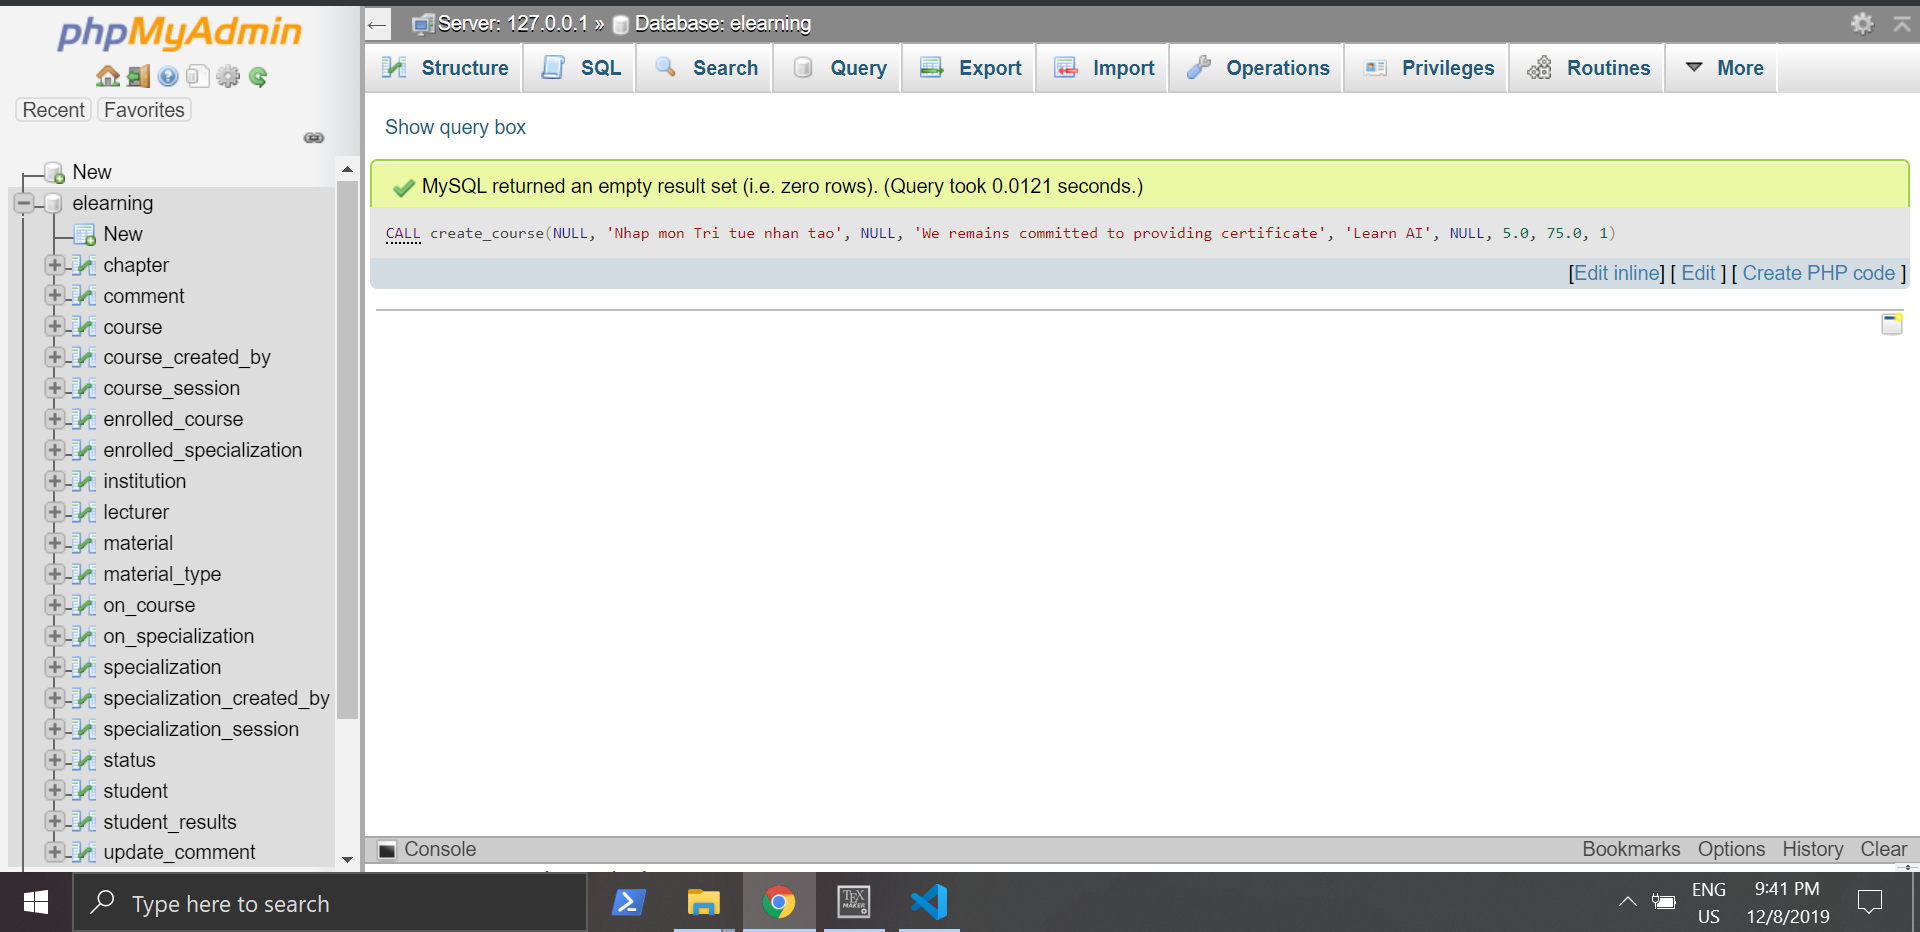
\includegraphics[width=0.8\textwidth]{images/p1s.png}
\end{figure}
\begin{figure}[h!]
	\centering
	\caption{Thực thi thủ tục insert course có lỗi}
	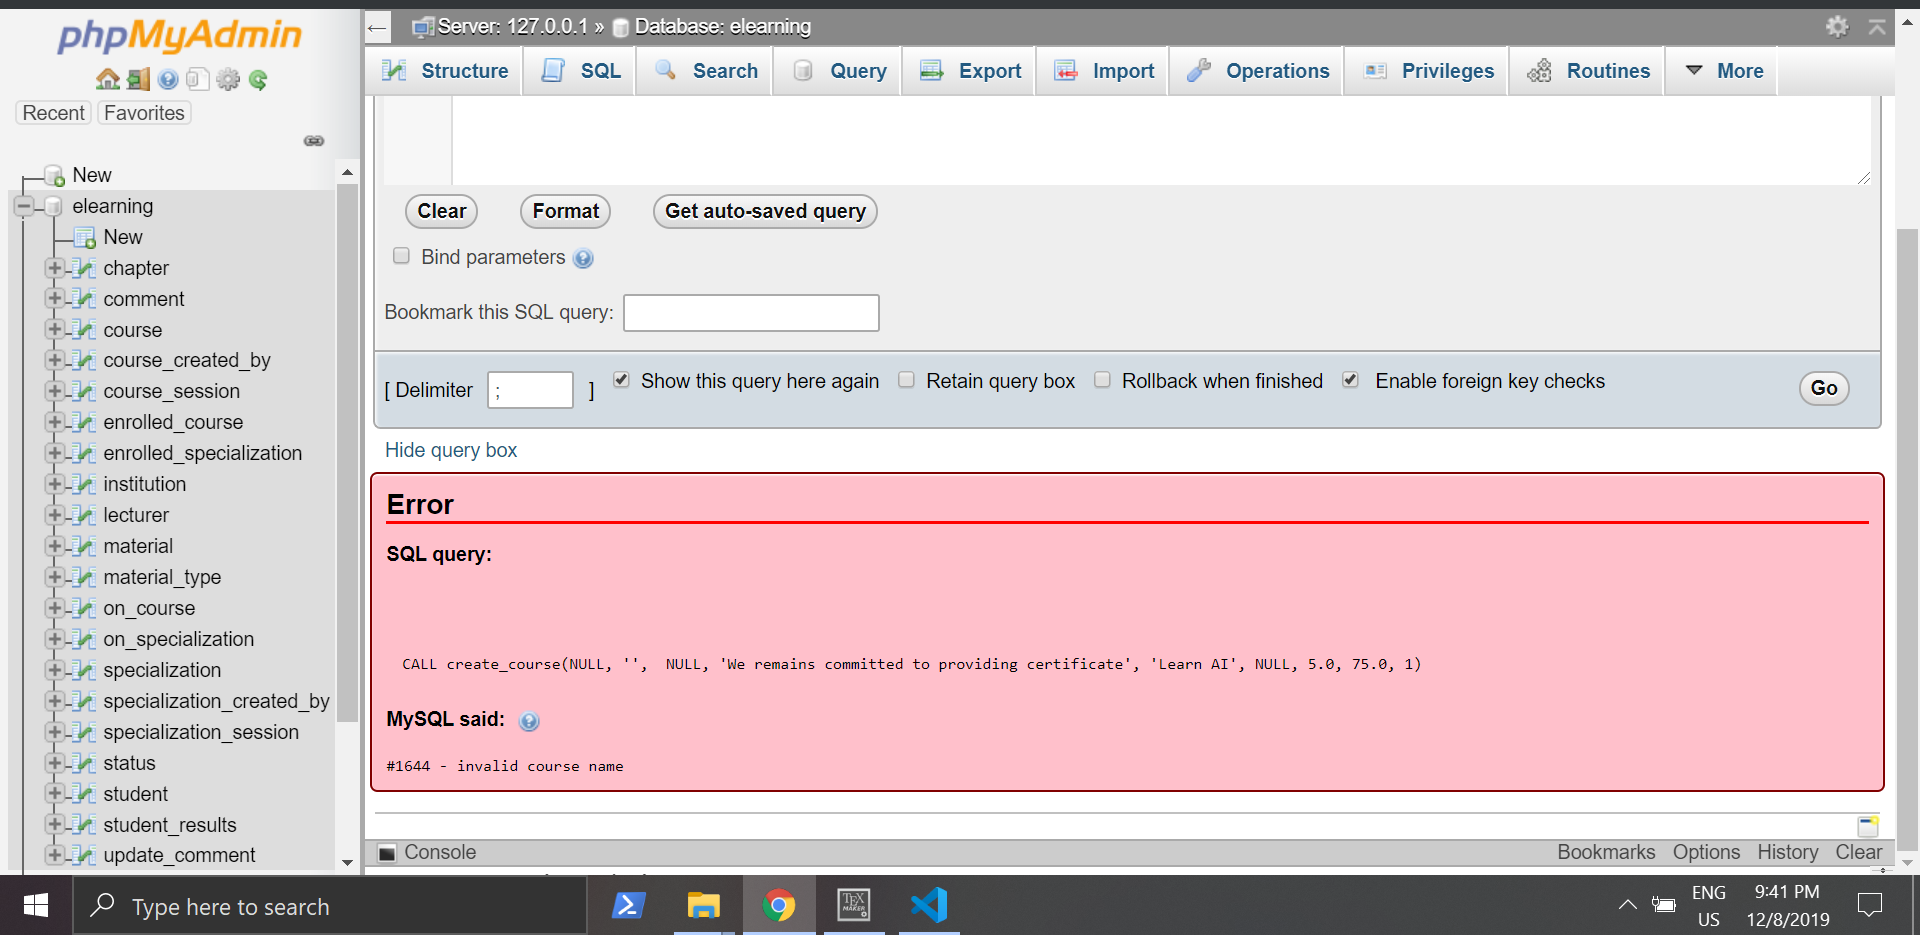
\includegraphics[width=0.8\textwidth]{images/p1e.png}
\end{figure}
\subsubsection{Trigger after insert course}
\textbf{$\bullet$ Mô tả chức năng:} Trigger sau khi thêm một hàng dữ liệu vào bảng course, sẽ kiểm tra xem điểm tối thiểu của khóa học (min_grade) và mã khóa học (nếu người dùng nhập cụ thể mã khóa học) có nằm trong khoảng giá trị cho phép không, nếu không thì báo lỗi. Ngoài ra trigger còn cập nhật số lượng khóa học trong mỗi lộ trình nếu insert một khóa học thuộc vào một lộ trình nào đó.\\
\textbf{$\bullet$ Lệnh tạo trigger:}
\begin{lstlisting}
DELIMITER $$
CREATE TRIGGER after_insert_course
AFTER INSERT ON `course`
FOR EACH ROW
BEGIN
	DECLARE c_id INT;
	DECLARE s_id INT;
	DECLARE c_min_grade DECIMAL(5,2);
	SET c_min_grade = NEW.min_grade;
	--
	IF(NEW.id IS NOT NULL)
	THEN
		SET c_id = NEW.id;
		IF(c_id < 0)
		THEN
			SIGNAL SQLSTATE '45000'
			SET MESSAGE_TEXT = 'course id could not be a negative integer';
		END IF;
	END IF;
	--
	IF(c_min_grade < 0.0) OR (c_min_grade > 10.0)
	THEN
		SIGNAL SQLSTATE '45000'
		SET MESSAGE_TEXT = 'min grade must in range [0.0, 10.0]';
	END IF;
	-- update number of courses in specialization
	IF (NEW.specialization_id IS NOT NULL)
	THEN
        SET s_id = NEW.specialization_id;
		UPDATE specialization SET num_of_courses = num_of_courses + 1 WHERE id = s_id;
	END IF;
END $$ 
DELIMITER ;
\end{lstlisting}
\textbf{$\bullet$ Lệnh kiểm tra trigger hoạt động:}
\begin{lstlisting}
CALL create_course(-60, 'Hoc may',  NULL, 'We remains committed to providing certificate', 'Learn Machine learning', NULL, 5.0, 75.0, 1);
CALL create_course(60, 'Hoc may',  NULL, 'We remains committed to providing certificate', 'Learn Machine learning', NULL, 10.5, 75.0, 1);
CALL create_course(NULL, 'Hoc may',  NULL, 'We remains committed to providing certificate', 'Learn Machine learning', NULL, 5.0, 75.0, 1);
\end{lstlisting}
\textbf{$\bullet$ Kết quả:}
\newpage
\begin{figure}[h!]
	\centering
	\caption{Báo lỗi vì nhập giá trị ngoài miền cho phép}
	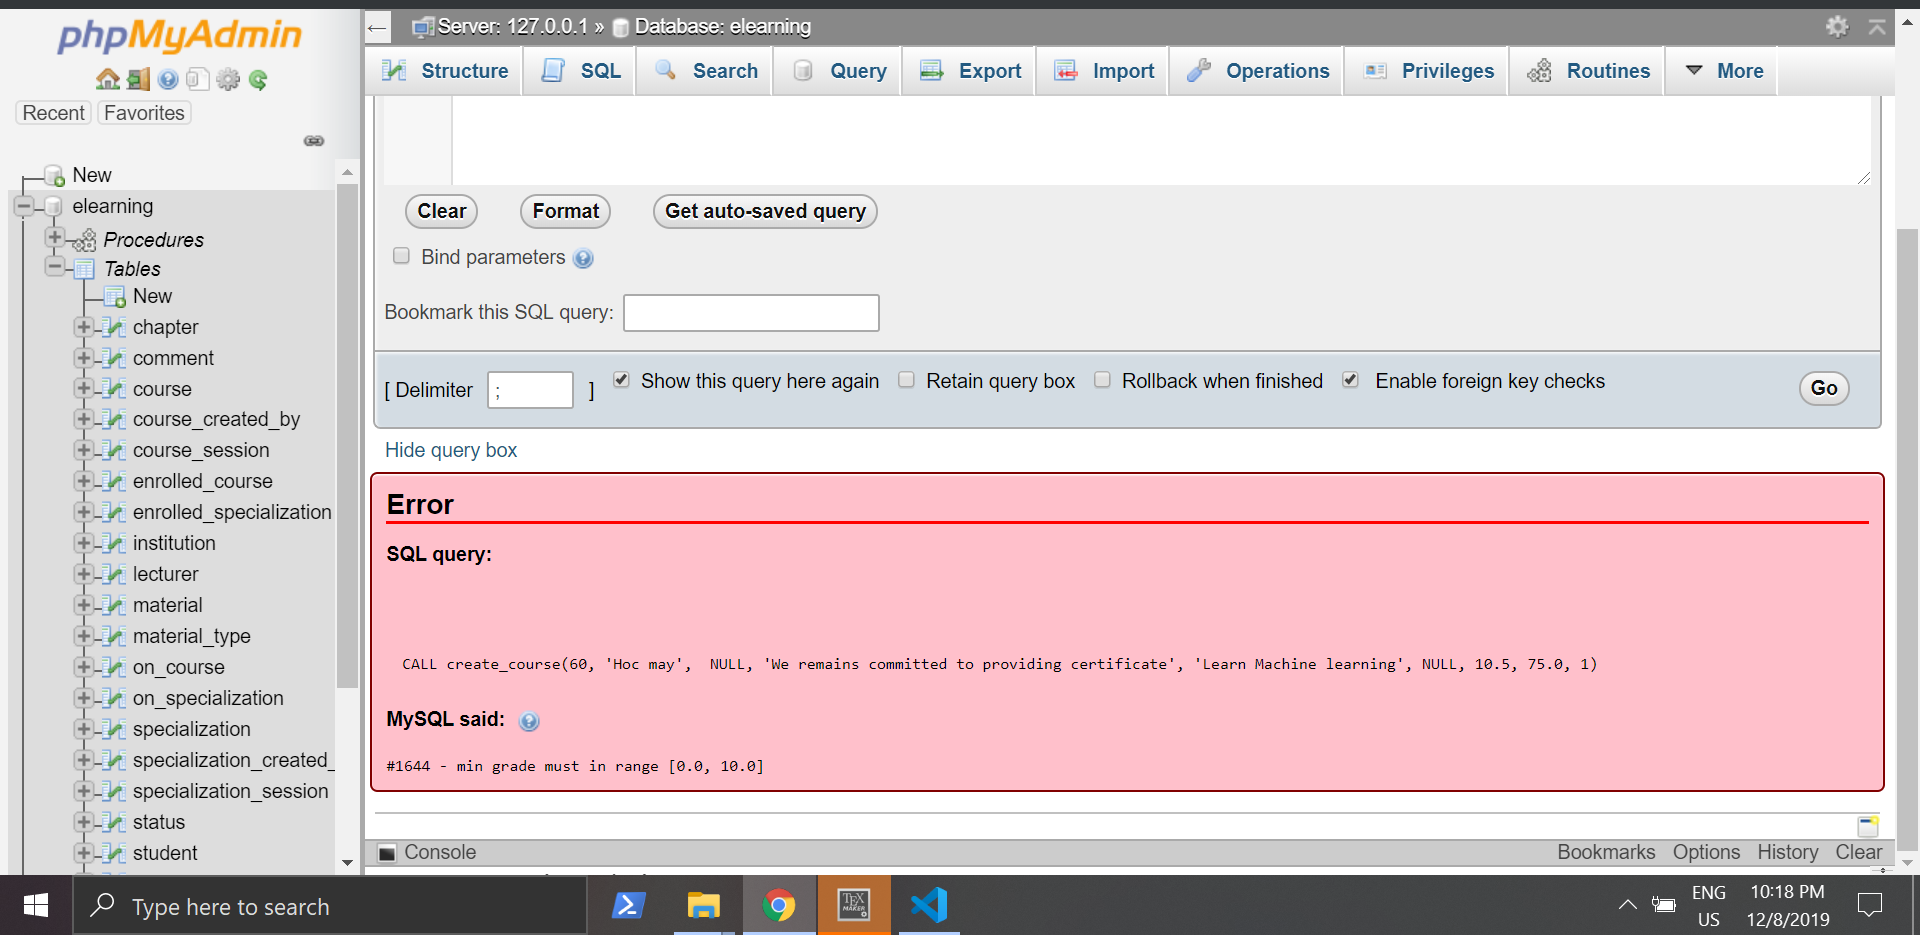
\includegraphics[width=0.8\textwidth]{images/triggerc1.png}
\end{figure}
\subsubsection{Trigger before delete course}
\textbf{$\bullet$ Mô tả chức năng:} Trigger này kiểm tra xem khóa học có ở trạng thái active hay không trước khi xóa, nếu khóa học đang ở trạng thái active thì không được phép xóa, ngoài ra nếu được phép xóa thì trigger sẽ kiểm tra xem khóa học bị xóa có thuộc lộ trình nào không, nếu có thì giảm số lượng khóa học trong lộ trình đó đi một.\\
\textbf{$\bullet$ Lệnh tạo trigger:}
\begin{lstlisting}
DELIMITER $$
CREATE TRIGGER before_delete_course
BEFORE DELETE ON `course`
FOR EACH ROW
BEGIN
    DECLARE c_status BIT;
    DECLARE s_id INT;
    SET c_status = OLD.active;
    IF(c_status = 1)
   	THEN
        SIGNAL SQLSTATE '45000'
		SET MESSAGE_TEXT = 'this course status is active, cannot delete this course';
    END IF;
    -- update number of courses in specialization
    IF (OLD.specialization_id IS NOT NULL)
	THEN
        SET s_id = OLD.specialization_id;
		UPDATE specialization SET num_of_courses = num_of_courses - 1 WHERE id = s_id;
	END IF;
END $$
DELIMITER ;
\end{lstlisting}
\newpage
\textbf{$\bullet$ Lệnh kiểm tra trigger hoạt động:}
\begin{lstlisting}
DELETE FROM `course` WHERE course.id = 50;

UPDATE `course` SET course.active = 0 WHERE course.id = 50;
DELETE FROM `course` WHERE course.id = 50;
\end{lstlisting}
\textbf{$\bullet$ Kết quả:}
\begin{figure}[h!]
	\centering
	\caption{Báo lỗi vì khóa học đang active}
	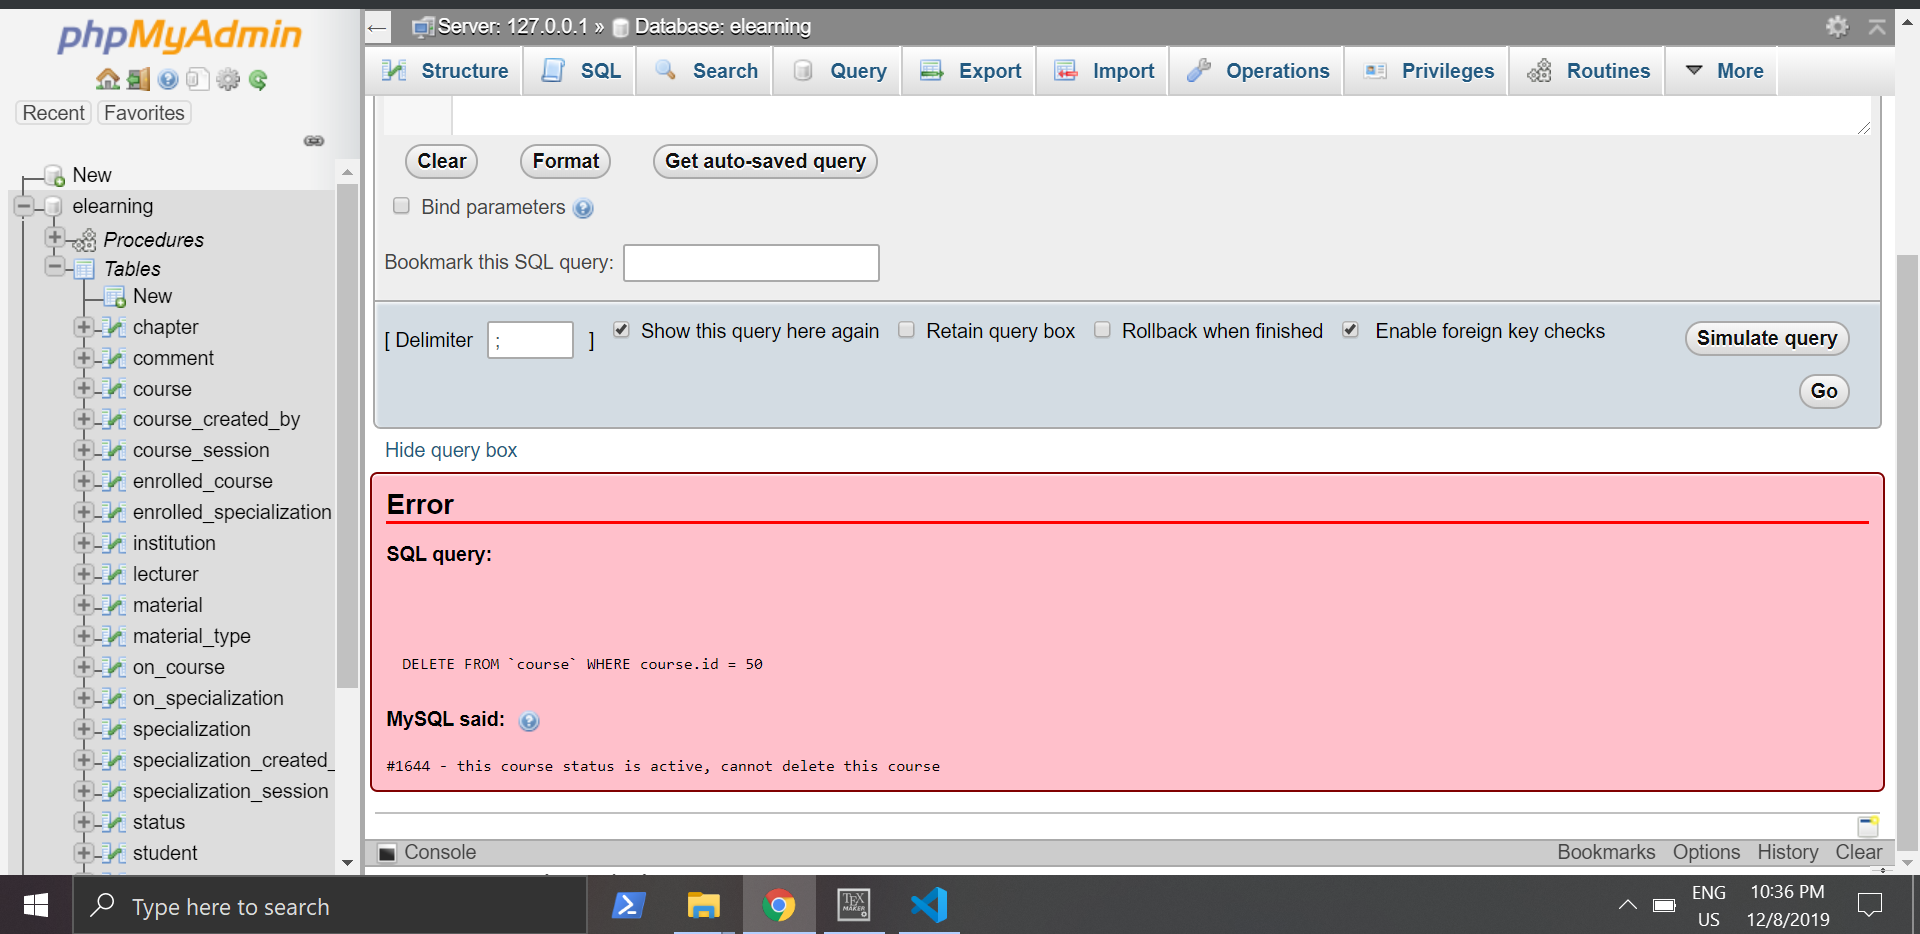
\includegraphics[width=0.8\textwidth]{images/triggerc2.png}
\end{figure}
\begin{figure}[h!]
	\centering
	\caption{Cập nhật trạng thái, trigger sẽ không chặn xóa khóa học nữa}
	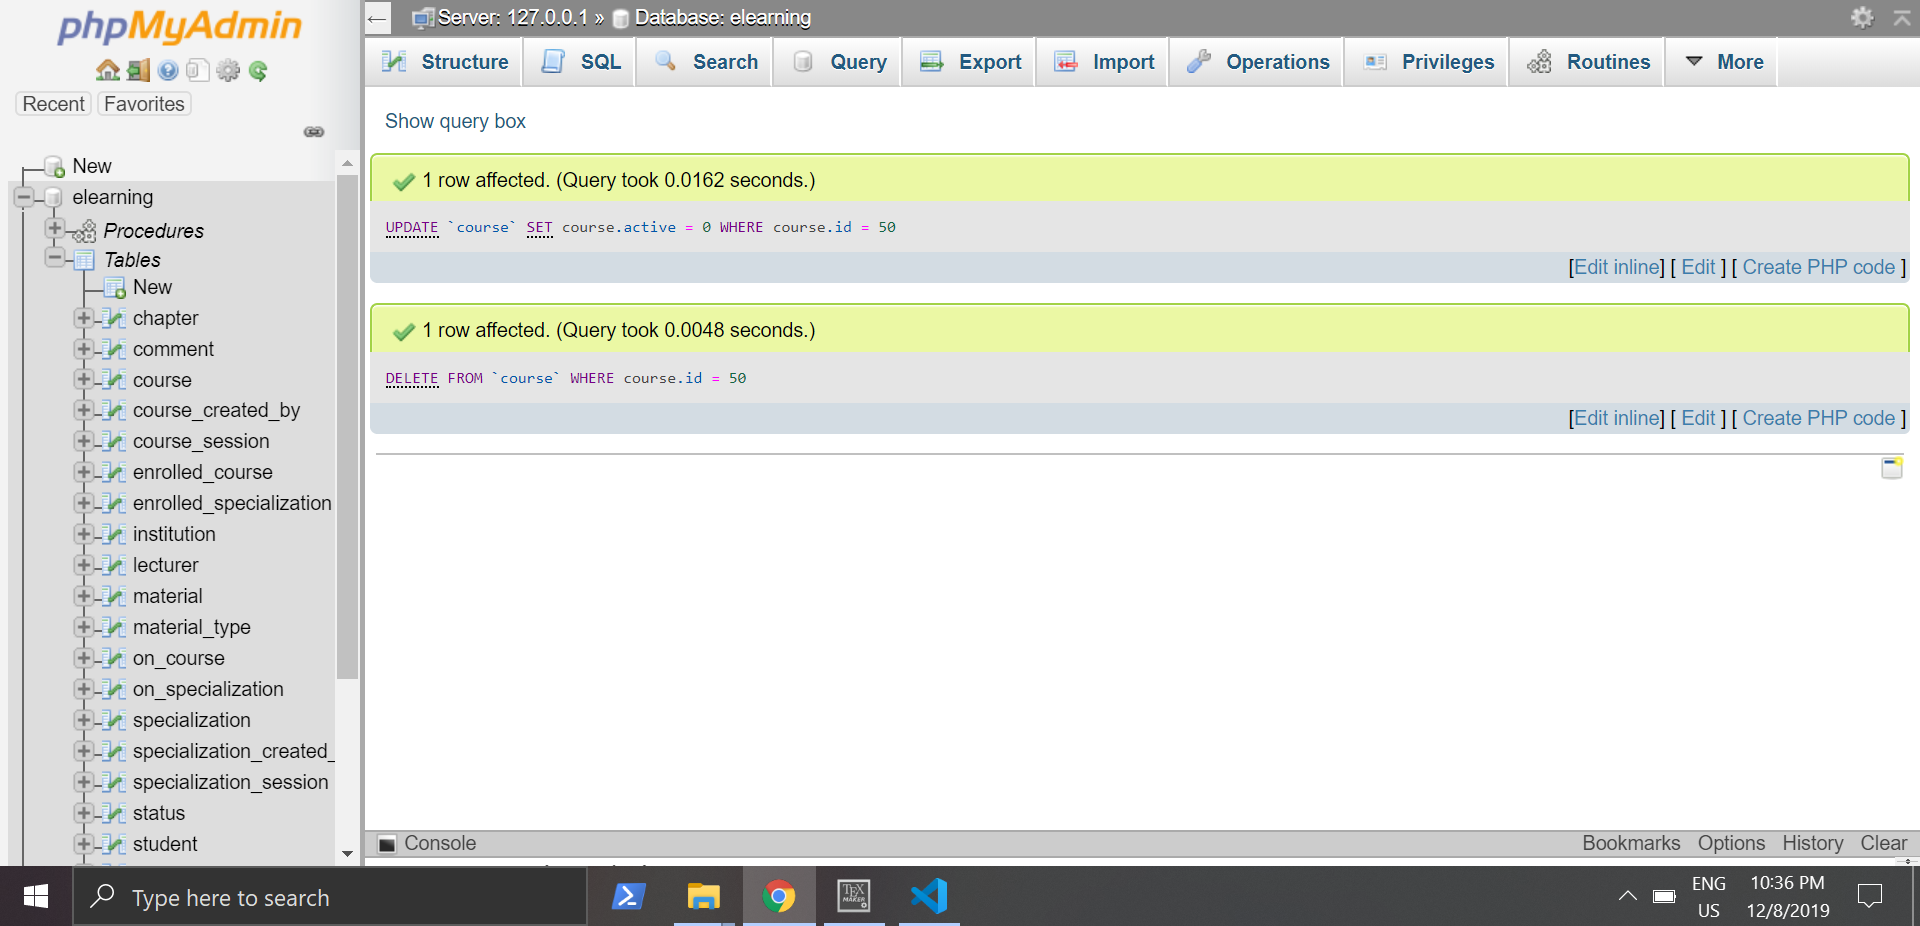
\includegraphics[width=0.8\textwidth]{images/triggerc3.png}
\end{figure}
\subsubsection{Thủ tục chứa câu truy vấn 1}
\textbf{$\bullet$ Mô tả chức năng:} Nhận vào một mã người học, câu truy vấn liệt kê ra các khóa học mà người đó đã đăng ký, bao gồm hình ảnh khóa học, tên khóa học và tổ chức tạo ra khóa học đó (sắp thứ tự theo tên khóa học).\\\\\\\\\\
\textbf{$\bullet$ Lệnh tạo thủ tục:}
\begin{lstlisting}
DELIMITER $$
CREATE PROCEDURE student_list_course
(
    IN std_id INT
)
BEGIN
	SELECT DISTINCT crs.image_url, crs.name, inst.name
	FROM `course` AS crs, `course_created_by` AS b, `institution` AS inst,
		`student` AS std, `enrolled_course` AS enr, `course_session` AS cs
	WHERE std.id = std_id
        AND b.course_id = crs.id
        AND b.institution_id = inst.id
        AND cs.course_id = crs.id
        AND enr.course_session_id = cs.id
        AND enr.student_id = std_id
	ORDER BY crs.name;
END $$
DELIMITER ;
\end{lstlisting}
\textbf{$\bullet$ Lệnh thực thi:}
\begin{lstlisting}
CALL student_list_course(2); -- 8 rows
CALL student_list_course(3); -- 4 rows
CALL student_list_course(5); -- no result
\end{lstlisting}
\textbf{$\bullet$ Kết quả:}
\begin{figure}[h!]
	\centering
	\caption{Truy vấn những khóa học của người học có id là 2}
	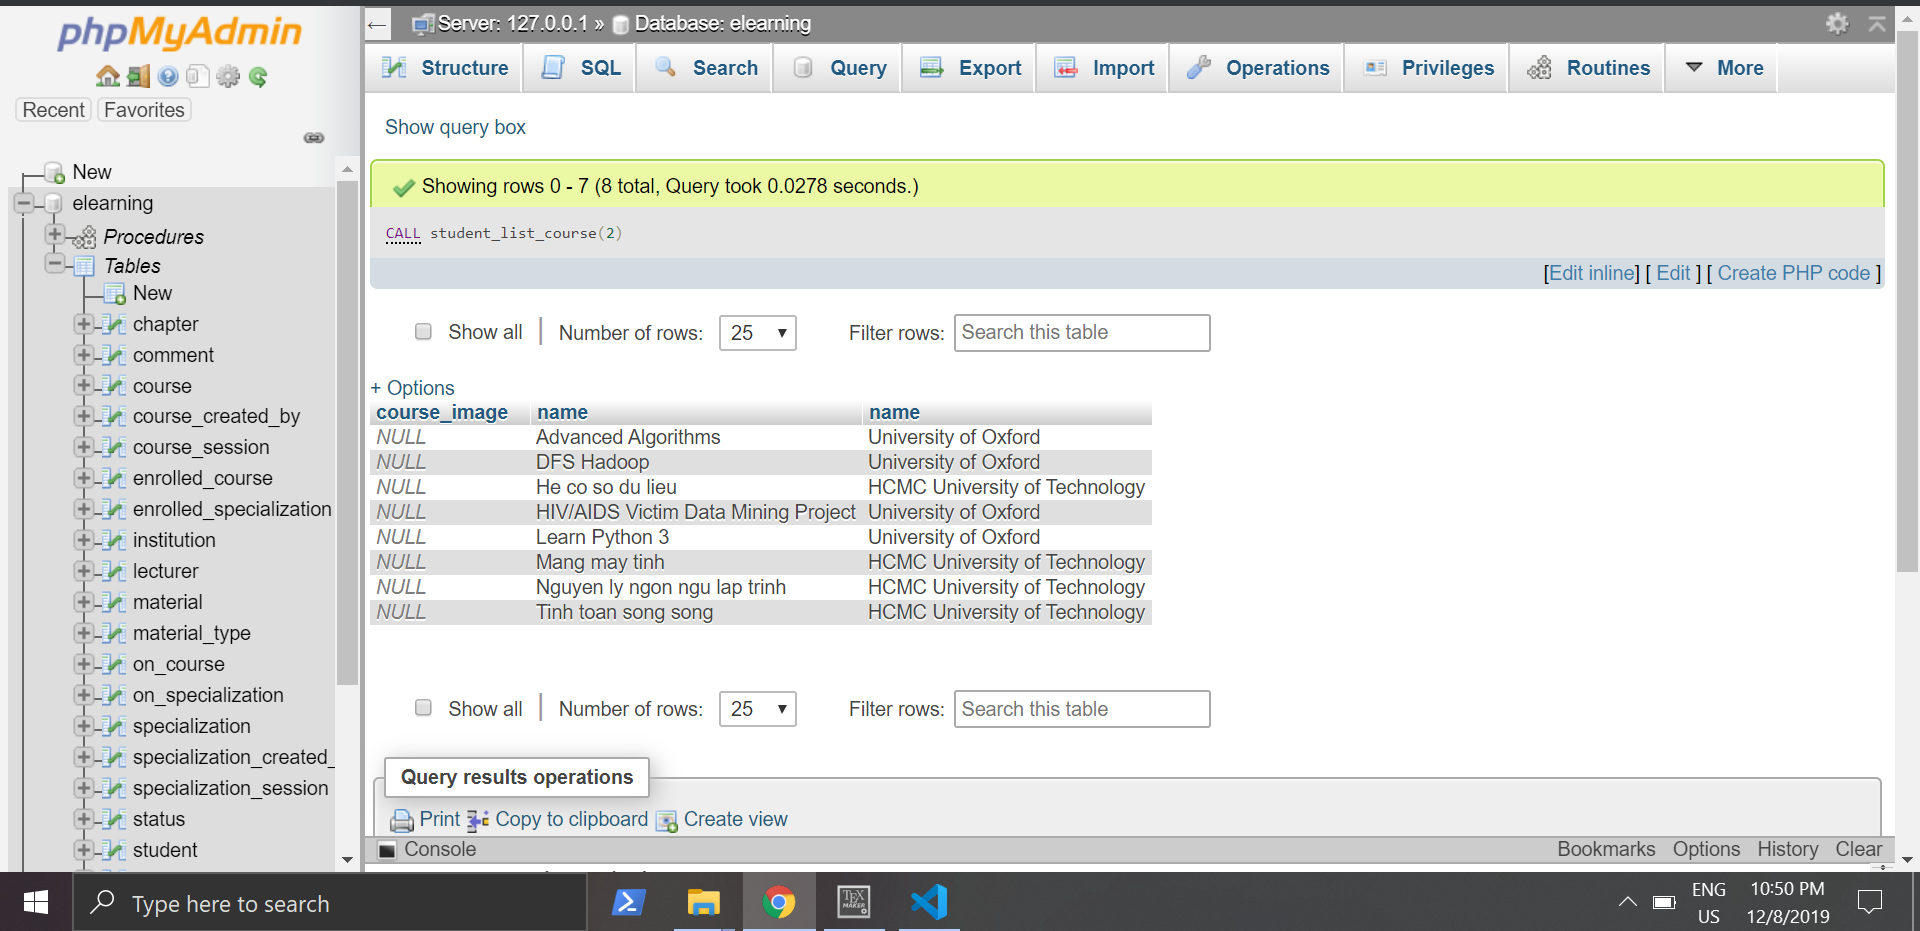
\includegraphics[width=0.8\textwidth]{images/proc1h.png}
\end{figure}
\newpage
\begin{figure}[h!]
	\centering
	\caption{Truy vấn những khóa học của người học có id là 5}
	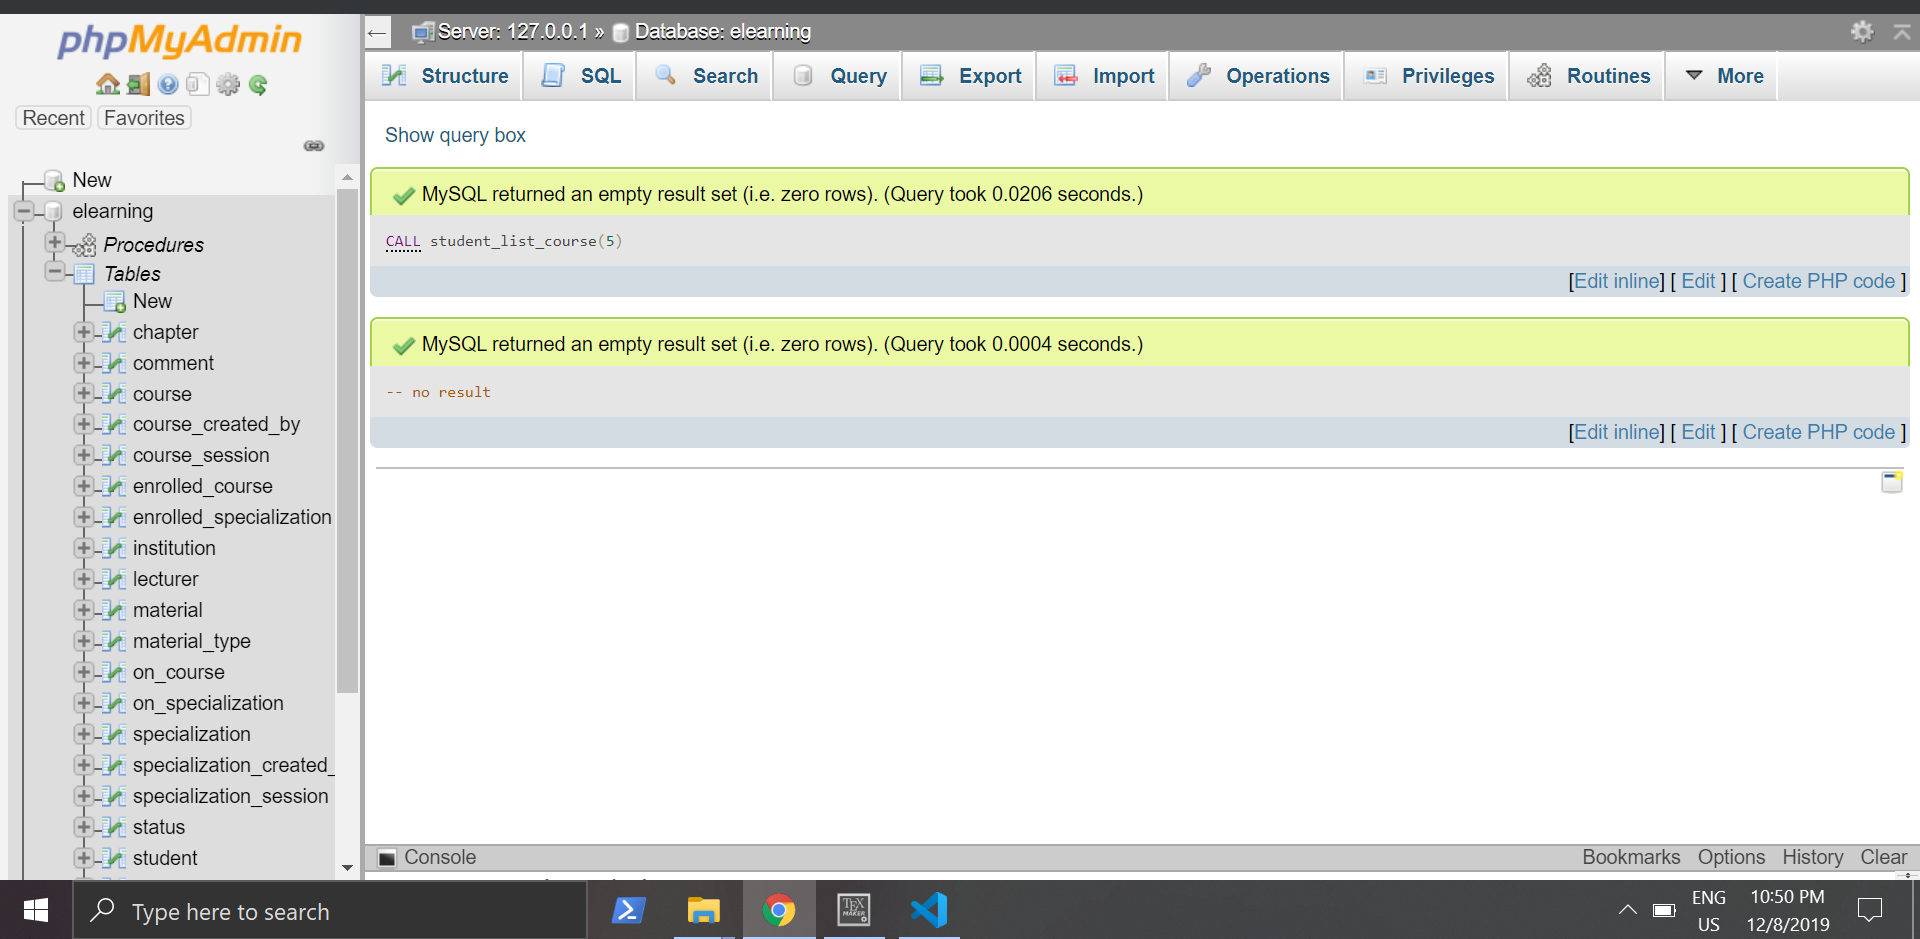
\includegraphics[width=0.8\textwidth]{images/proc1nh.png}
\end{figure}
\subsubsection{Thủ tục chứa câu truy vấn 2}
\textbf{$\bullet$ Mô tả chức năng:} Thủ tục nhận vào một mã người học và một định giá, thủ tục truy vấn tổng tiền mà người dùng đã bỏ ra để mua khóa học ứng với từng tổ chức và có tổng tiền chi ra lớn hơn định giá đã nhập vào, kết quả được sắp xếp theo mã tổ chức.\\
\textbf{$\bullet$ Lệnh tạo thủ tục:}
\begin{lstlisting}
DELIMITER $$
CREATE PROCEDURE student_course_summary
(
    IN std_id INT,
    total DECIMAL(8,2)
)
BEGIN
	SELECT inst.name AS 'institution name', COUNT(*) AS 'bought course', SUM(crs.course_price) AS 'total paid'
	FROM `course` AS crs, `course_created_by` AS b, `institution` AS inst,
        `student` AS std, `enrolled_course` AS enr, `course_session` AS cs
	WHERE std.id = std_id
        AND b.course_id = crs.id
        AND b.institution_id = inst.id
        AND cs.course_id = crs.id
        AND enr.course_session_id = cs.id
        AND enr.student_id = std_id
    GROUP BY inst.id
    HAVING (SUM(crs.course_price) > total)
	ORDER BY inst.id;
END $$
DELIMITER ;
\end{lstlisting}
\textbf{$\bullet$ Lệnh thực thi:}
\begin{lstlisting}
CALL student_course_summary(2, 100.0);
CALL student_course_summary(2, 200.0);
CALL student_course_summary(4, 100.0);
CALL student_course_summary(5, 100.0);
\end{lstlisting}
\textbf{$\bullet$ Kết quả:}
\begin{figure}[h!]
	\centering
	\caption{Tổng tiền mua khóa học của người học có id là 2, số tiền chi lớn hơn 100 đô}
	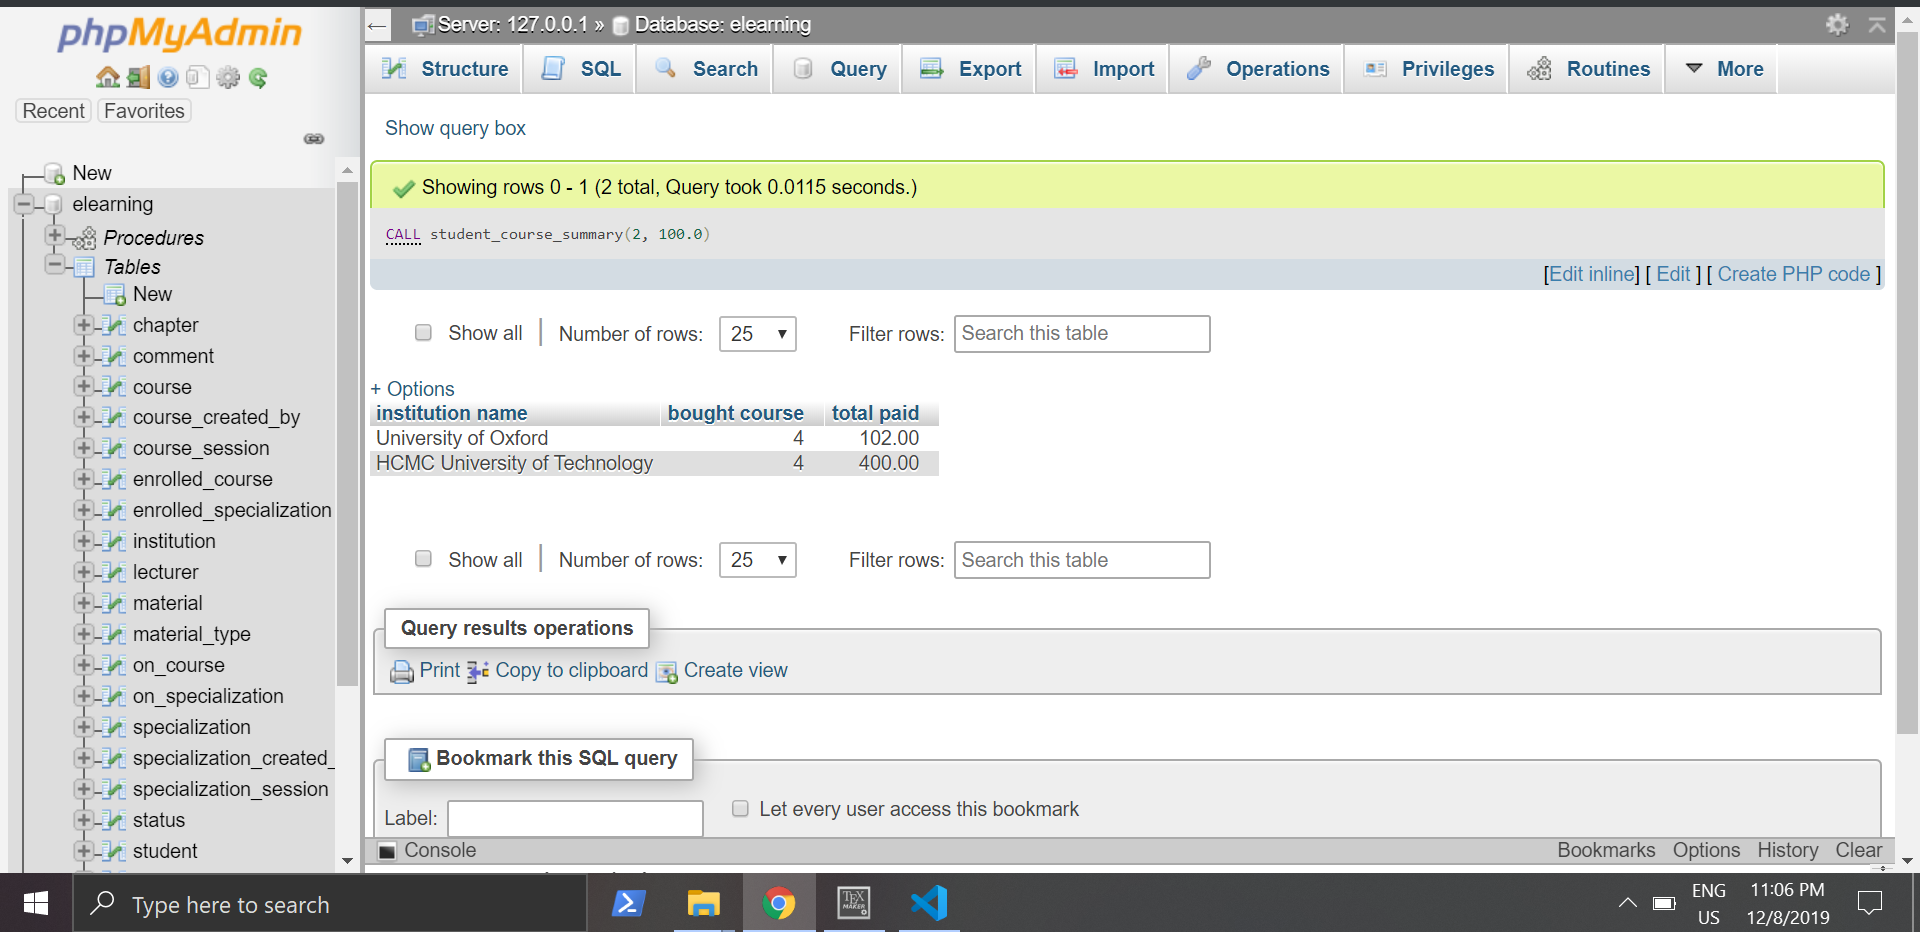
\includegraphics[width=0.8\textwidth]{images/onehun.png}
\end{figure}
\begin{figure}[h!]
	\centering
	\caption{Tổng tiền mua khóa học của người học có id là 2, số tiền chi lớn hơn 200 đô}
	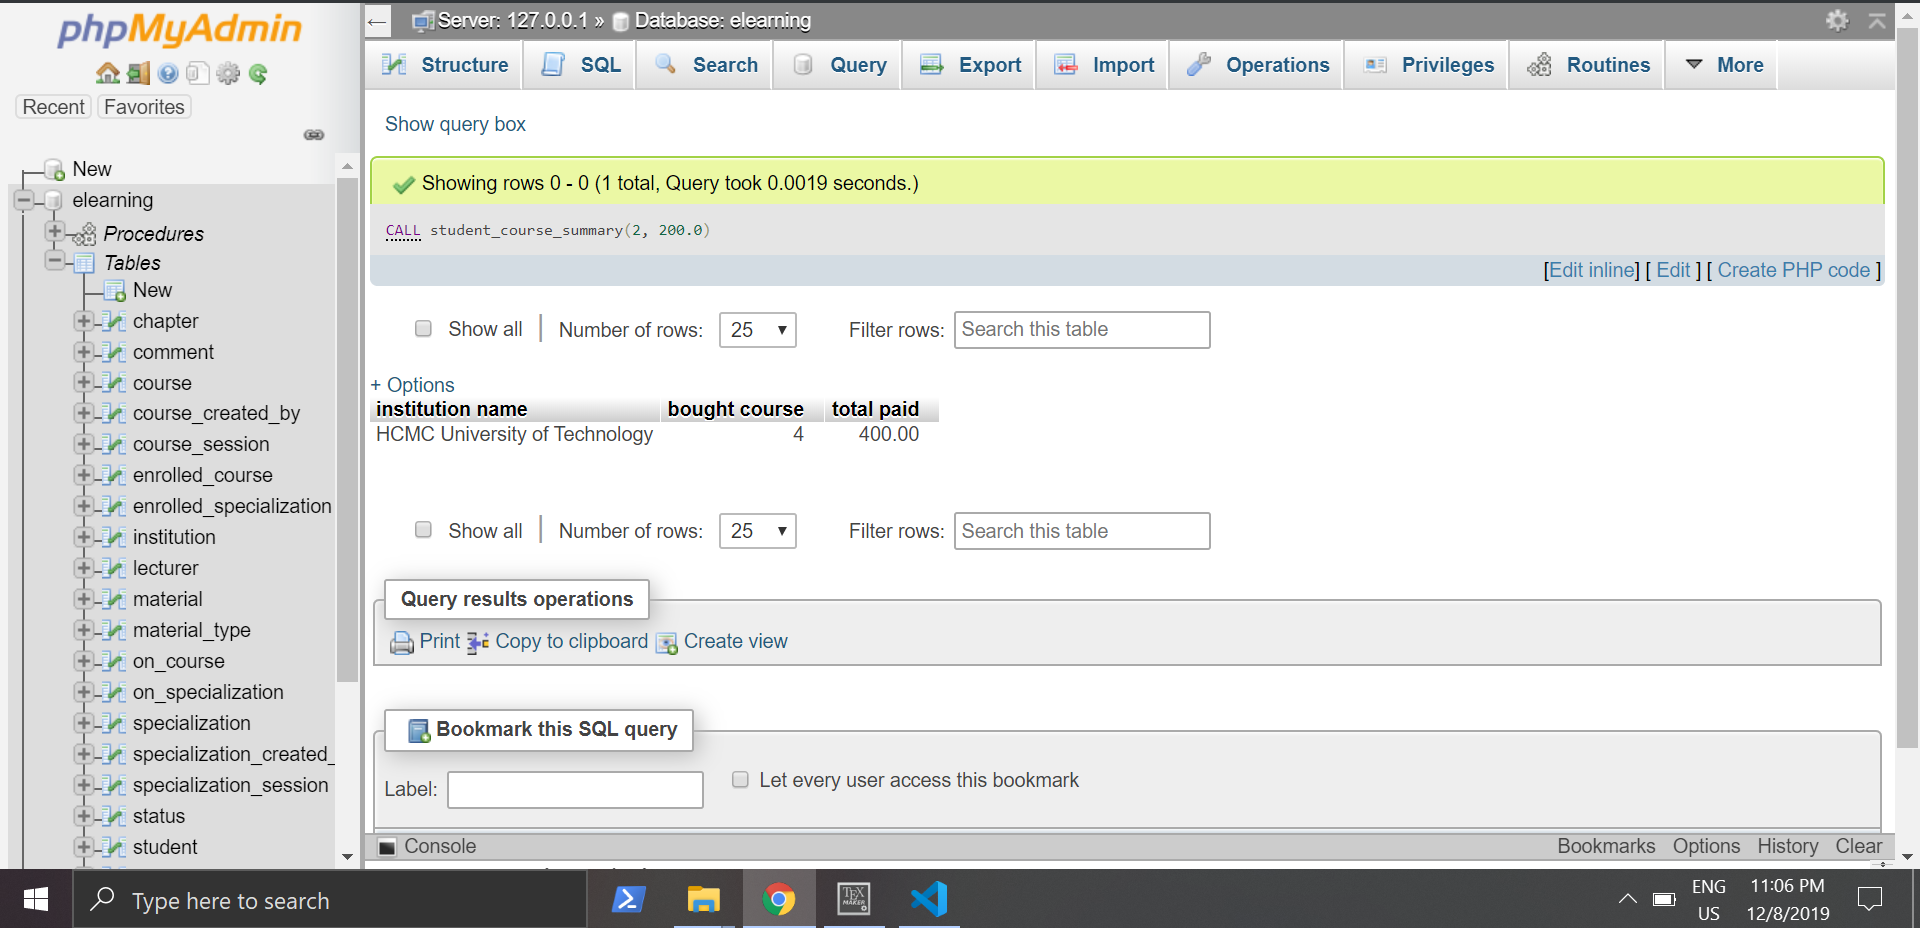
\includegraphics[width=0.8\textwidth]{images/twohun.png}
\end{figure}
\subsubsection{Hàm 1}
\textbf{$\bullet$ Mô tả chức năng:} Hàm nhận vào một mã lộ trình, tính toán trả về phí đăng ký lộ trình đó thông qua giá của các khóa học thuộc về lộ trình và discount của lộ trình đó.\\
\textbf{$\bullet$ Lệnh tạo hàm:}
\begin{lstlisting}
DELIMITER $$
CREATE FUNCTION specialization_price(s_id INT) RETURNS DECIMAL(8,2)
BEGIN
	DECLARE finished BIT;
	DECLARE partial DECIMAL(8,2);
	DECLARE total DECIMAL(8,2) DEFAULT 0.0;
	DECLARE sale DECIMAL(8,2);
	DECLARE this_cursor CURSOR FOR (SELECT course.course_price FROM `course` WHERE course.specialization_id = s_id);
	DECLARE CONTINUE HANDLER FOR NOT FOUND SET finished = 1;
	--
	IF ((SELECT COUNT(*) FROM `specialization` WHERE specialization.id = s_id) = 0)
	THEN
		SIGNAL SQLSTATE '45000'
		SET MESSAGE_TEXT = 'specialization not found';
		RETURN 0.0;
	END IF;
	--
	SET sale = (SELECT specialization.specialization_discount FROM `specialization` WHERE specialization.id = s_id);
	OPEN this_cursor;
	reduce: LOOP
		FETCH this_cursor INTO partial;
		IF (finished = 1)
		THEN
			LEAVE reduce;
		END IF;
		SET total = total + partial;
	END LOOP;
	CLOSE this_cursor;
	RETURN total - sale;
END $$
DELIMITER ;
\end{lstlisting}
\textbf{$\bullet$ Câu lệnh SELECT minh họa gọi hàm:}
\begin{lstlisting}
SELECT spec.id, spec.name, spec.specialization_discount, spec.num_of_courses, specialization_price(spec.id) AS 'price'
FROM `specialization` AS spec
WHERE id = 1
\end{lstlisting}
\textbf{$\bullet$ Kết quả:}
\newpage
\begin{figure}[h!]
	\centering
	\caption{Giá của lộ trình có id là 1}
	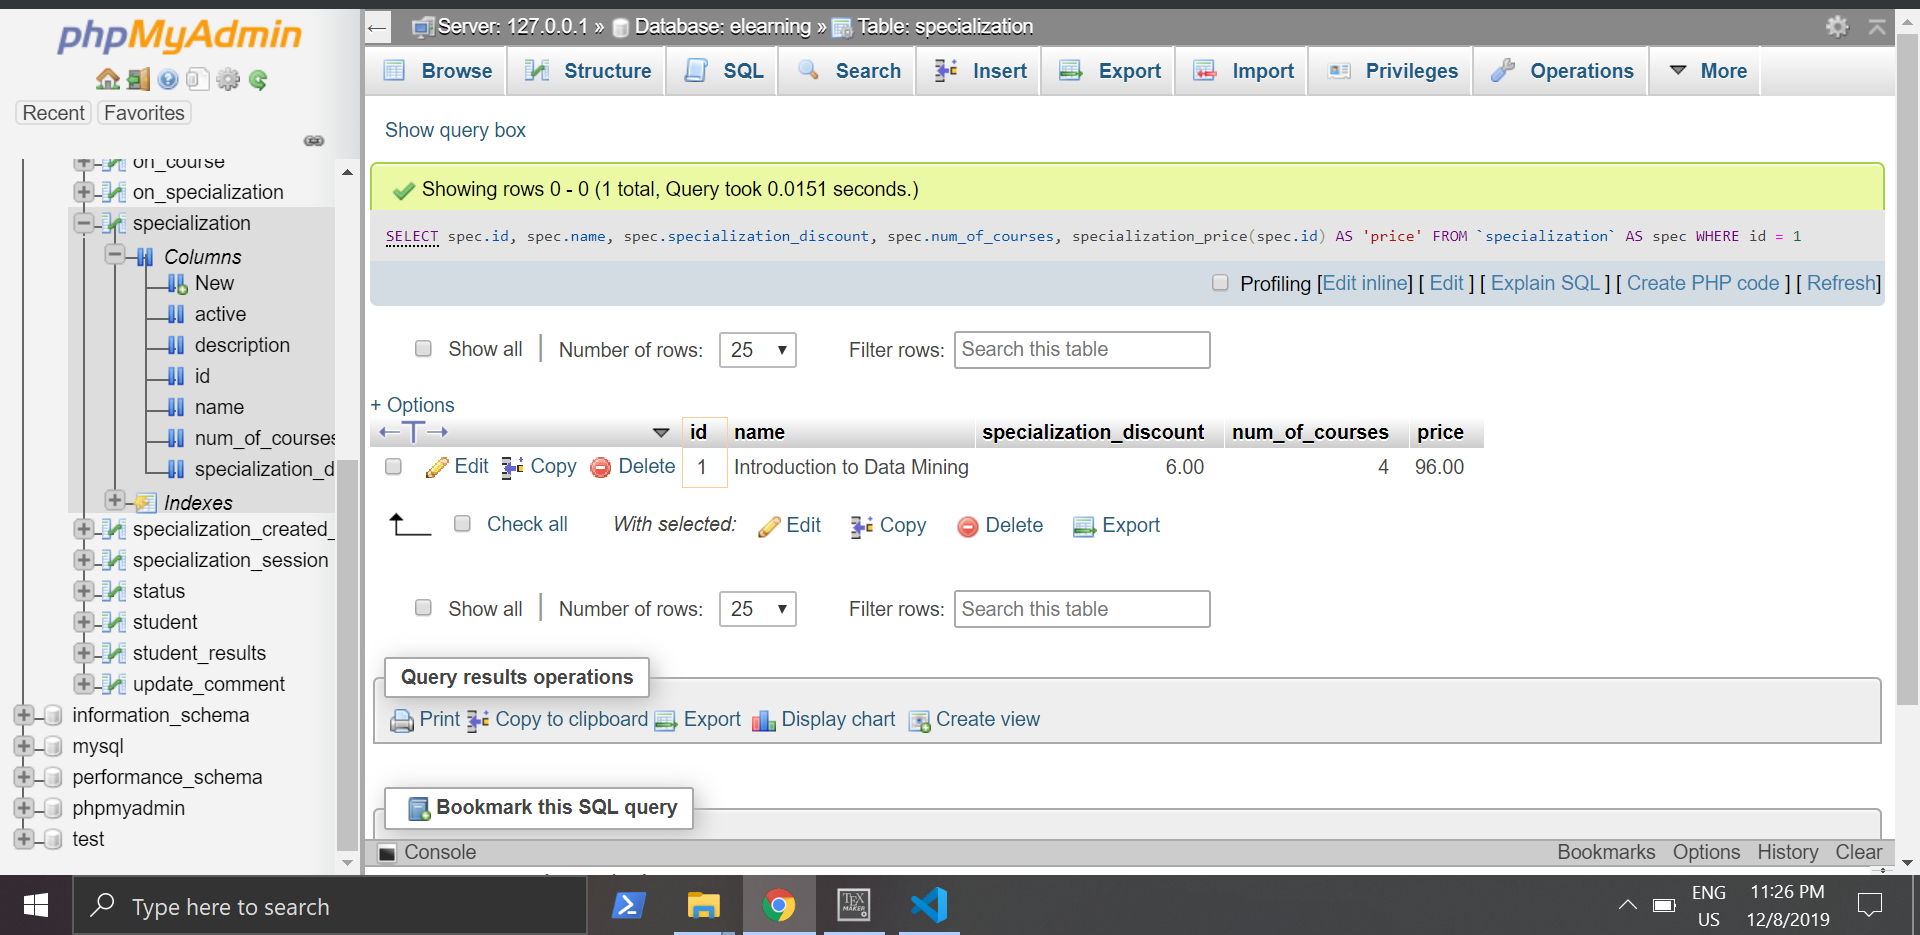
\includegraphics[width=0.8\textwidth]{images/specprice.png}
\end{figure}
\subsubsection{Hàm 2}
\textbf{$\bullet$ Mô tả chức năng:} Hàm nhận vào một mã khóa học, hàm trả về doanh thu của khóa học đó.\\
\textbf{$\bullet$ Lệnh tạo hàm:}
\begin{lstlisting}
DELIMITER $$
CREATE FUNCTION total_course_sold(c_id INT) RETURNS DECIMAL(8,2)
BEGIN
    DECLARE number_of_courses DECIMAL(8,2) DEFAULT 0.0;
    DECLARE c_price DECIMAL(8,2);
    --
    IF ((SELECT COUNT(*) FROM `course` WHERE course.id = c_id) = 0)
    THEN
    	SIGNAL SQLSTATE '45000'
		SET MESSAGE_TEXT = 'course not found';
		RETURN 0.0;
    END IF;
    --
    SET c_price = (SELECT course.course_price FROM `course` WHERE course.id = c_id);
    --
    SET number_of_courses = (
        SELECT COUNT(*) FROM `enrolled_course`, `course_session`
        WHERE course_session.course_id = c_id
            AND enrolled_course.course_session_id = course_session.id
    );
    RETURN number_of_courses * c_price;
END $$
DELIMITER ;
\end{lstlisting}
\textbf{$\bullet$ Câu lệnh SELECT minh họa gọi hàm:}
\newpage
\begin{lstlisting}
SELECT crs.id, crs.name, total_course_sold(crs.id) AS 'total sold'
FROM `course` AS crs
WHERE id = 38
\end{lstlisting}
\textbf{$\bullet$ Kết quả:}
\begin{figure}[h!]
	\centering
	\caption{Tổng doanh thu của khóa Cơ sở dữ liệu}
	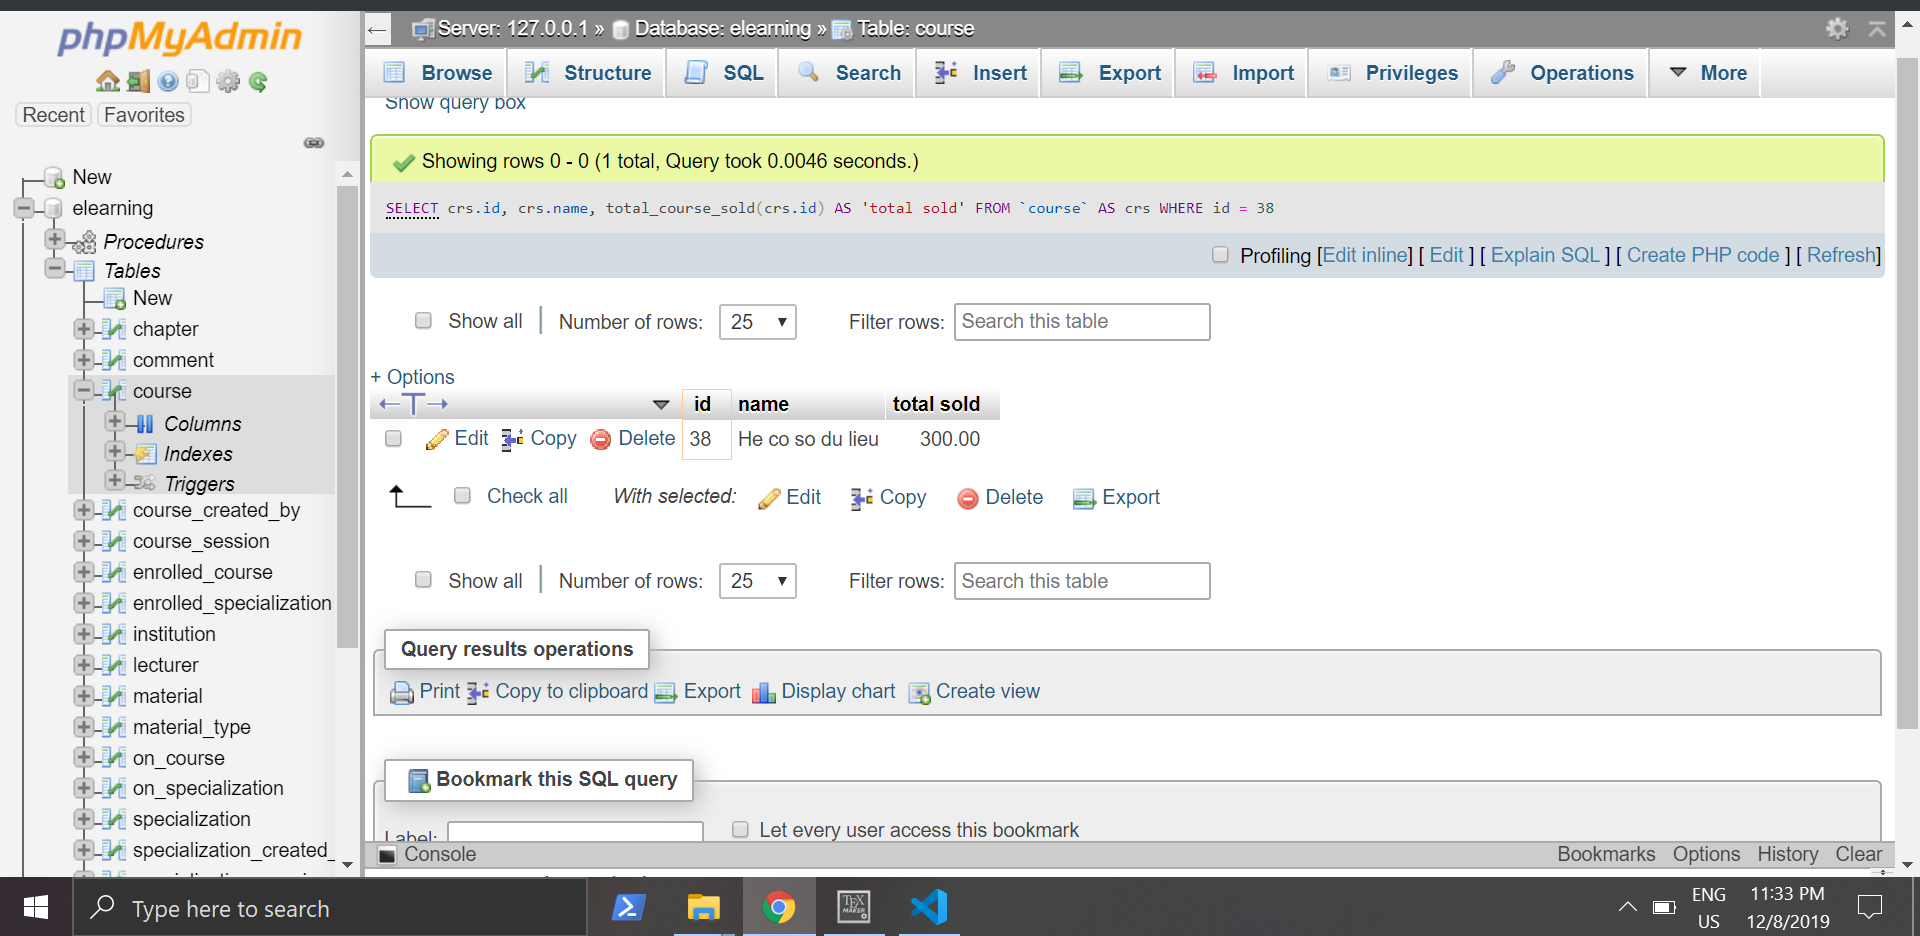
\includegraphics[width=0.8\textwidth]{images/course_sold.png}
\end{figure}
\subsubsection{Giao diện ứng dụng và các hình ảnh minh họa}
\begin{figure}[h!]
	\centering
	\caption{Danh sách các khóa học}
	
\includegraphics[width=0.35\textwidth]{images/course1.png}
\end{figure}
\newpage
\begin{figure}[h!]
	\centering
	\caption{Thông tin giới thiệu khóa học}
	
\includegraphics[width=0.35\textwidth]{images/course2.png}
\end{figure}
\newpage
\subsection{Thao tác với bảng dữ liệu comment}
\textit{Thành viên 2: Dương Văn Tài, MSSV: 1613001}
\subsubsection{Thủ tục Insert dữ liệu}
\textbf{$\bullet$ Mô tả chức năng:} Cho phép insert dữ liệu vào bảng comment với inputs là các trường dữ liệu cần nhập. Thân thủ tục sẽ kiểm tra mã khóa học, mã người học có phải là NULL hay không, nếu là NULL thì sẽ thông báo lỗi. Nếu comment không chứa nội dung thì cũng sẽ báo lỗi. Đối với mã comment, nếu người dùng nhập NULL thì sẽ được tăng theo AUTO_INCREMENT, còn nếu nhập mã cụ thể thì sẽ insert mã cụ thể đó.\\
\textbf{$\bullet$ Lệnh tạo thủ tục:}
\begin{lstlisting}
DELIMITER $$
CREATE PROCEDURE create_comment
(
	cmmt_id int,
	crs_id varchar(255),
	std_id varchar(255),
	cmmt_content text,
    c_time datetime
)
BEGIN
	IF (crs_id IS NULL)
	THEN
		SIGNAL SQLSTATE '45000'
		SET MESSAGE_TEXT = 'invalid course id';
	END IF;
	--
	IF (std_id IS NULL)
	THEN
		SIGNAL SQLSTATE '45000'
		SET MESSAGE_TEXT = 'invalid student id';
	END IF;
	--
	IF (cmmt_content IS NULL OR LENGTH(cmmt_content) = 0)
	THEN
		SIGNAL SQLSTATE '45000'
		SET MESSAGE_TEXT = 'comment have no content';
	END IF;
	-- insert into course table
	IF (cmmt_id IS NULL)
	THEN
		INSERT INTO `comment` VALUES(NULL, crs_id, std_id, cmmt_content, c_time);
	ELSE
		INSERT INTO `comment` VALUES(cmmt_id, crs_id, std_id, cmmt_content, c_time);
	END IF;
END $$
DELIMITER ;
\end{lstlisting}
\textbf{$\bullet$ Lệnh thực thi:}
\begin{lstlisting}
CALL create_comment(NULL, 37, 2, 'hello!', NOW());
CALL create_comment(35, 37, 2, 'hello!', NOW());
\end{lstlisting}
\textbf{$\bullet$ Kết quả:}
\begin{figure}[h!]
	\centering
	\caption{Thực thi thủ tục insert comment thành công}
	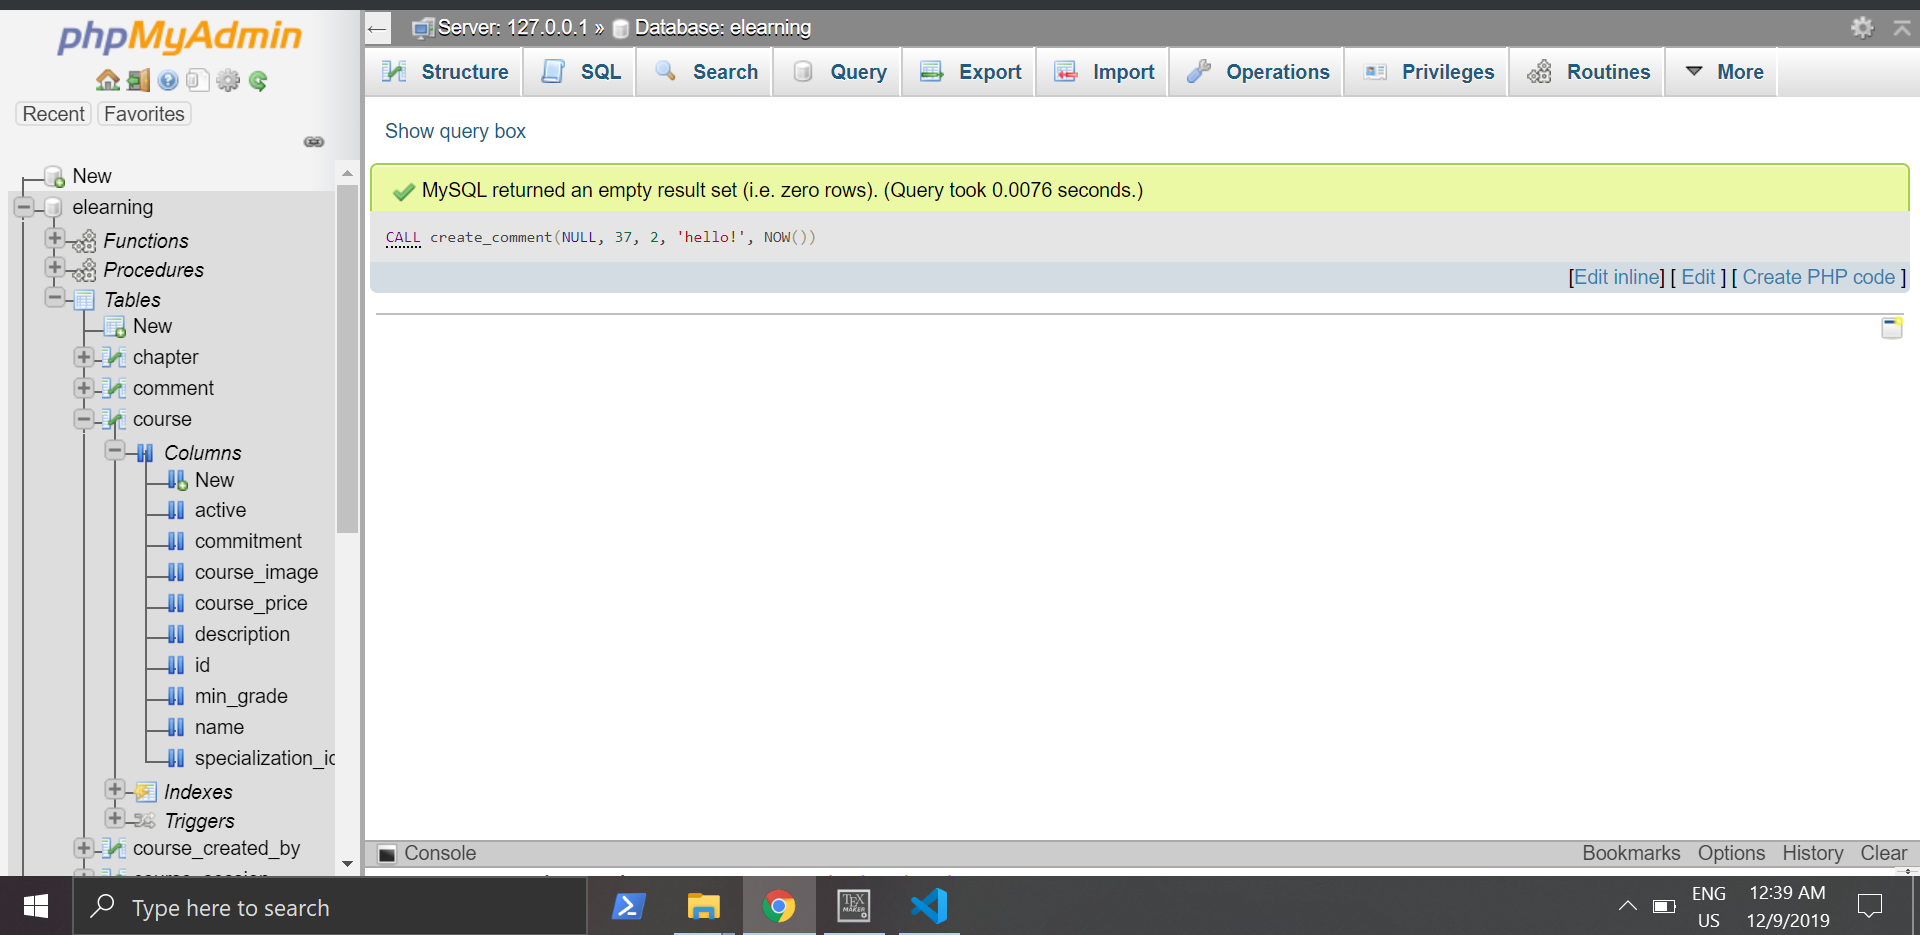
\includegraphics[width=0.8\textwidth]{images/cmmt1.png}
\end{figure}
\subsubsection{Trigger before insert comment}
\textbf{$\bullet$ Mô tả chức năng:} Trigger chặn không cho người dùng comment quá 20 lần một ngày vào cùng một khóa học để tránh người dùng spam.\\
\textbf{$\bullet$ Lệnh tạo trigger:}
\begin{lstlisting}
DELIMITER $$
CREATE TRIGGER before_insert_comment
BEFORE INSERT ON `comment`
FOR EACH ROW
BEGIN
    DECLARE crs_id INT;
    DECLARE std_id INT;
    DECLARE c_time date;
    DECLARE commented INT;
    SET crs_id = NEW.course_id;
    SET std_id = NEW.student_id;
    SET c_time = DATE(NEW.cmmt_time);
    --
    SET commented = (
        SELECT COUNT(*) FROM `comment`
        WHERE course_id = crs_id
        AND student_id = std_id
        AND DATE(cmmt_time) = c_time
    );
    IF(commented = 20)
    THEN
        SIGNAL SQLSTATE '45000'
		SET MESSAGE_TEXT = 'cannot comment';
    END IF;
END $$
DELIMITER ;
\end{lstlisting}
\textbf{$\bullet$ Lệnh kiểm tra trigger hoạt động:}
\begin{lstlisting}
CALL create_comment(NULL, 37, 2, 'spam', NOW());
\end{lstlisting}
\textbf{$\bullet$ Kết quả:}
\begin{figure}[h!]
	\centering
	\caption{Báo lỗi khi tạo comment thứ 21}
	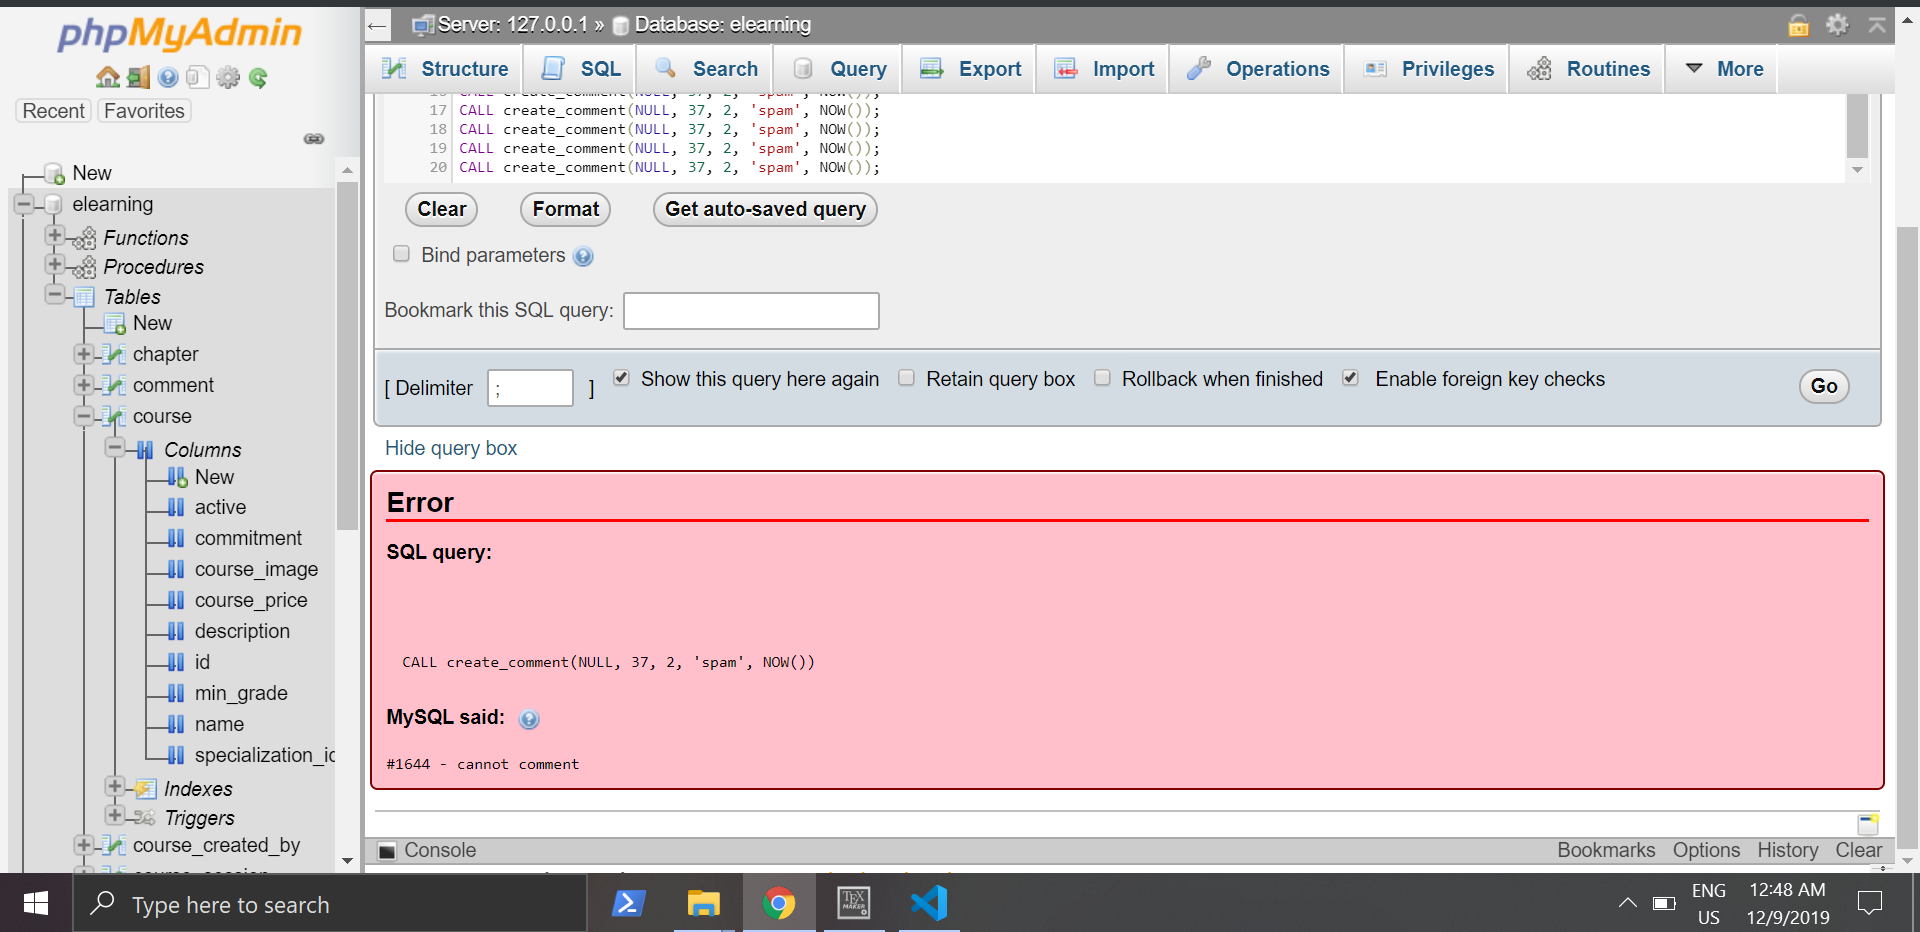
\includegraphics[width=0.8\textwidth]{images/cmmt2.png}
\end{figure}
\subsubsection{Trigger after update comment}
\textbf{$\bullet$ Mô tả chức năng:} Trigger này lưu lạy lịch sử cập nhật comment của người dùng vào bảng update_comment mỗi khi người dùng cập nhật comment của mình.\\
\textbf{$\bullet$ Lệnh tạo trigger:}
\begin{lstlisting}
DELIMITER $$
CREATE TRIGGER after_update_comment
AFTER UPDATE ON `comment`
FOR EACH ROW
BEGIN
	INSERT INTO `update_comment`
    VALUES(NULL, OLD.id, OLD.content, OLD.cmmt_time);
END $$
DELIMITER ;
\end{lstlisting}
\textbf{$\bullet$ Lệnh kiểm tra trigger hoạt động:}
\begin{lstlisting}
UPDATE `comment` SET content = 'co cho diem rat cao', cmmt_time = NOW()
WHERE id = 10;
UPDATE `comment` SET content = 'co cho diem rat rat cao', cmmt_time = NOW()
WHERE id = 10;
UPDATE `comment` SET content = 'ma cung hen xui nua', cmmt_time = NOW()
WHERE id = 10;
SELECT * FROM `update_comment`
WHERE comment_id = 10
ORDER BY cmmt_time;

SELECT * FROM `comment`
WHERE id = 10;
\end{lstlisting}
\textbf{$\bullet$ Kết quả:}
\begin{figure}[h!]
	\centering
	\caption{Truy vấn lịch sử sửa comment}
	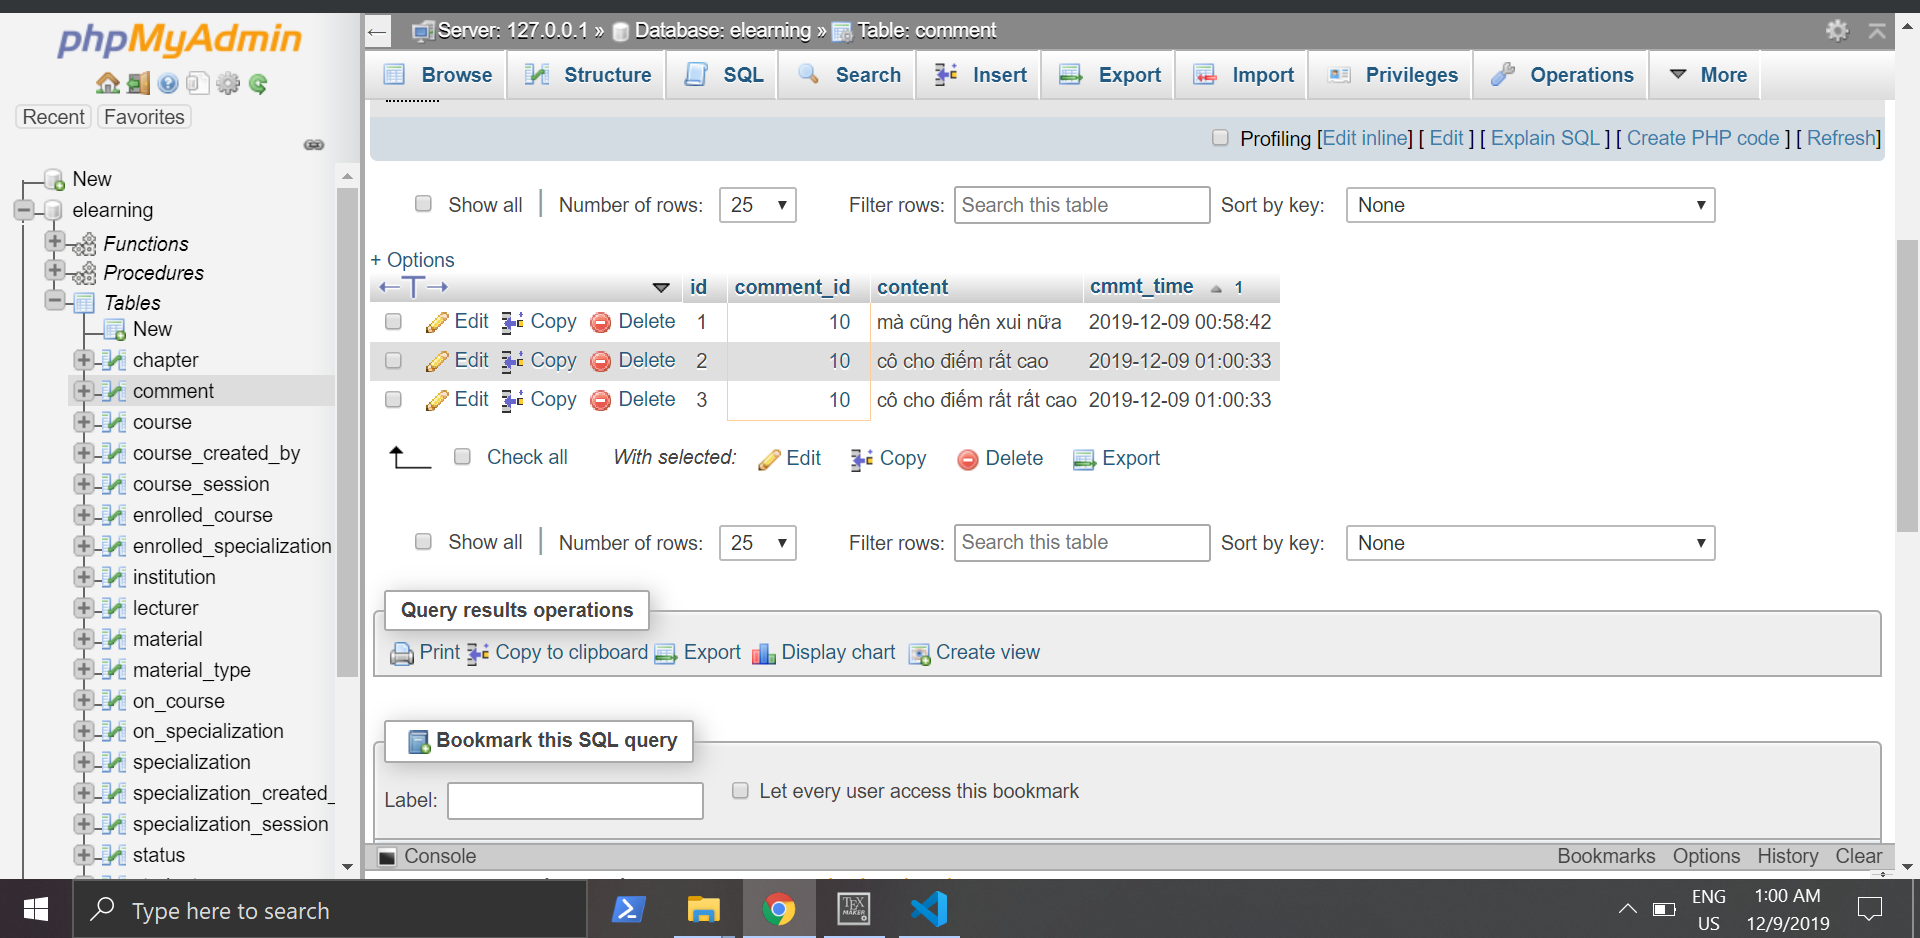
\includegraphics[width=0.8\textwidth]{images/cmmt3.png}
\end{figure}
\begin{figure}[h!]
	\centering
	\caption{Comment mới nhất được update}
	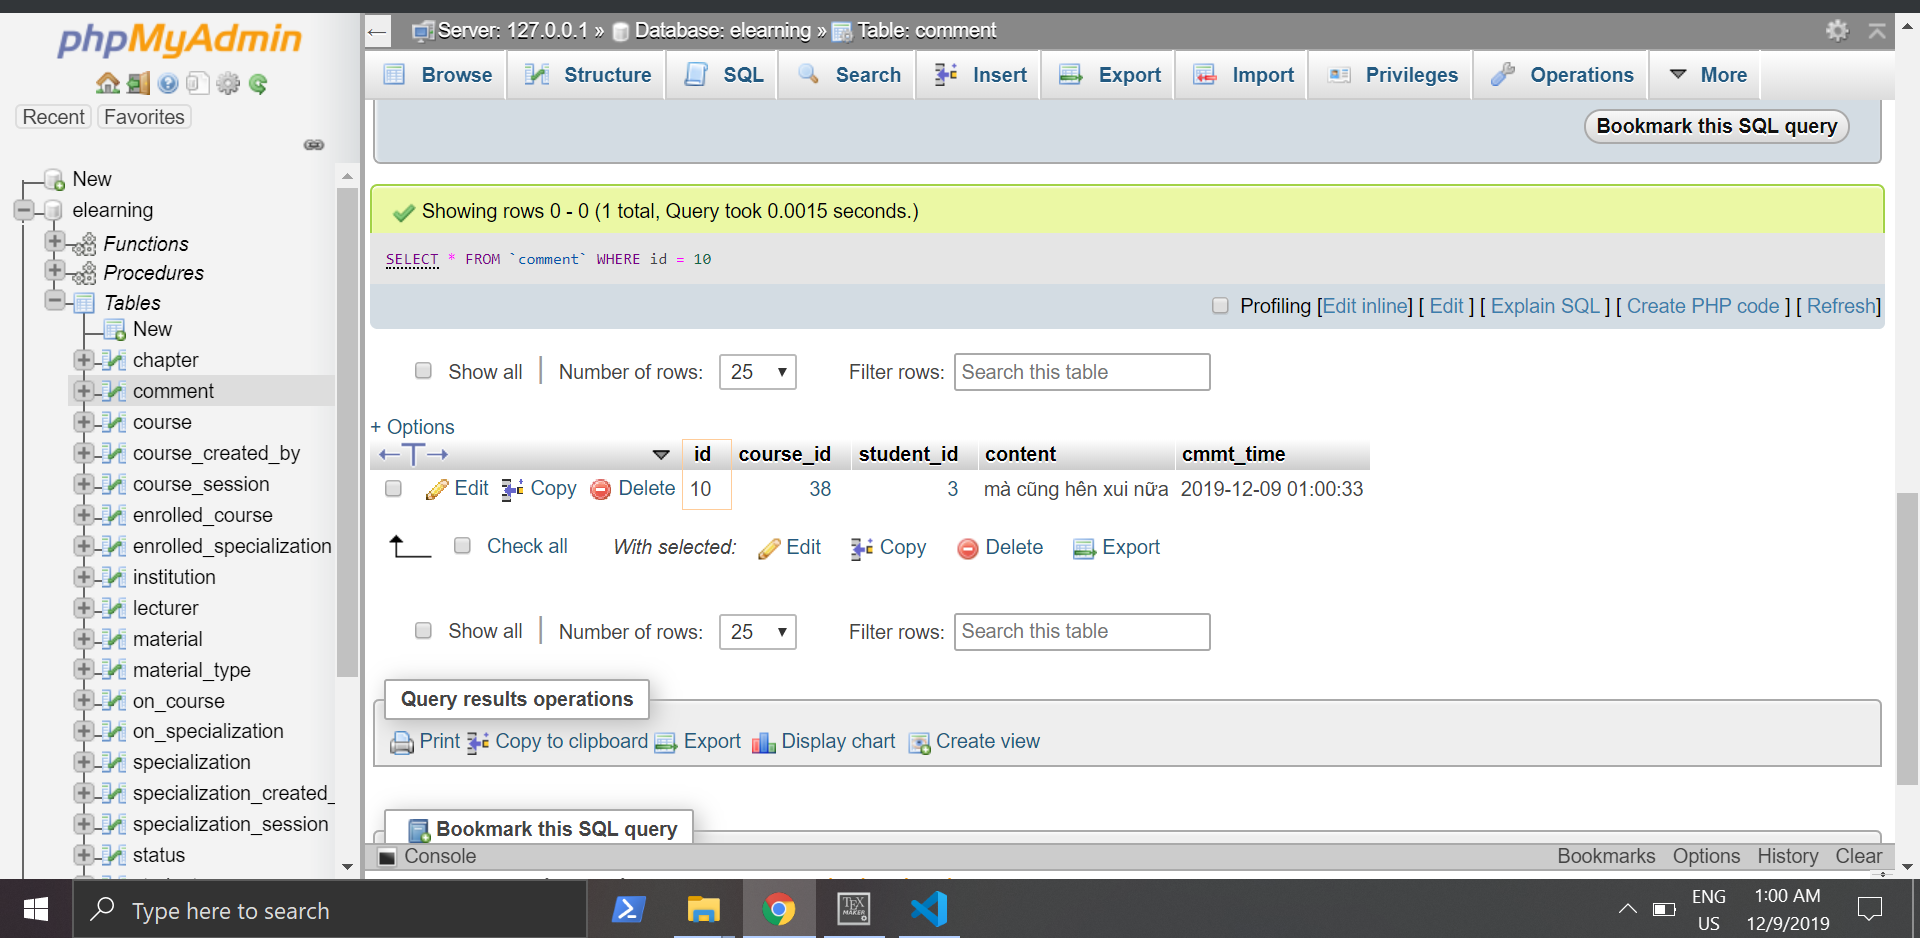
\includegraphics[width=0.8\textwidth]{images/cmmt4.png}
\end{figure}
\subsubsection{Thủ tục chứa câu truy vấn 1}
\textbf{$\bullet$ Mô tả chức năng:} Nhận vào mã khóa học, truy vấn danh sách comment của khóa học đó bao gồm mã comment, nội dung, thời gian comment, mã người comment, tên và ảnh của người comment.\\
\textbf{$\bullet$ Lệnh tạo thủ tục:}
\begin{lstlisting}
DELIMITER $$
CREATE PROCEDURE get_comments(IN course_id int, IN off_set INT) 
BEGIN
  SELECT cmt.id, cmt.content, cmt.cmmt_time, s.id, s.last_name, s.first_name, s.image_url
  FROM comment cmt
  INNER JOIN student s ON cmt.student_id = s.id
  WHERE 
  cmt.course_id = course_id
  ORDER BY
  cmt.id
  LIMIT
    off_set, 20;
END $$
DELIMITER ;
\end{lstlisting}
\textbf{$\bullet$ Lệnh thực thi:}
\begin{lstlisting}
CALL get_comments(38, 0);
\end{lstlisting}
\textbf{$\bullet$ Kết quả:}
\begin{figure}[h!]
	\centering
	\caption{Truy vấn danh sách comment của khóa học có id là 38}
	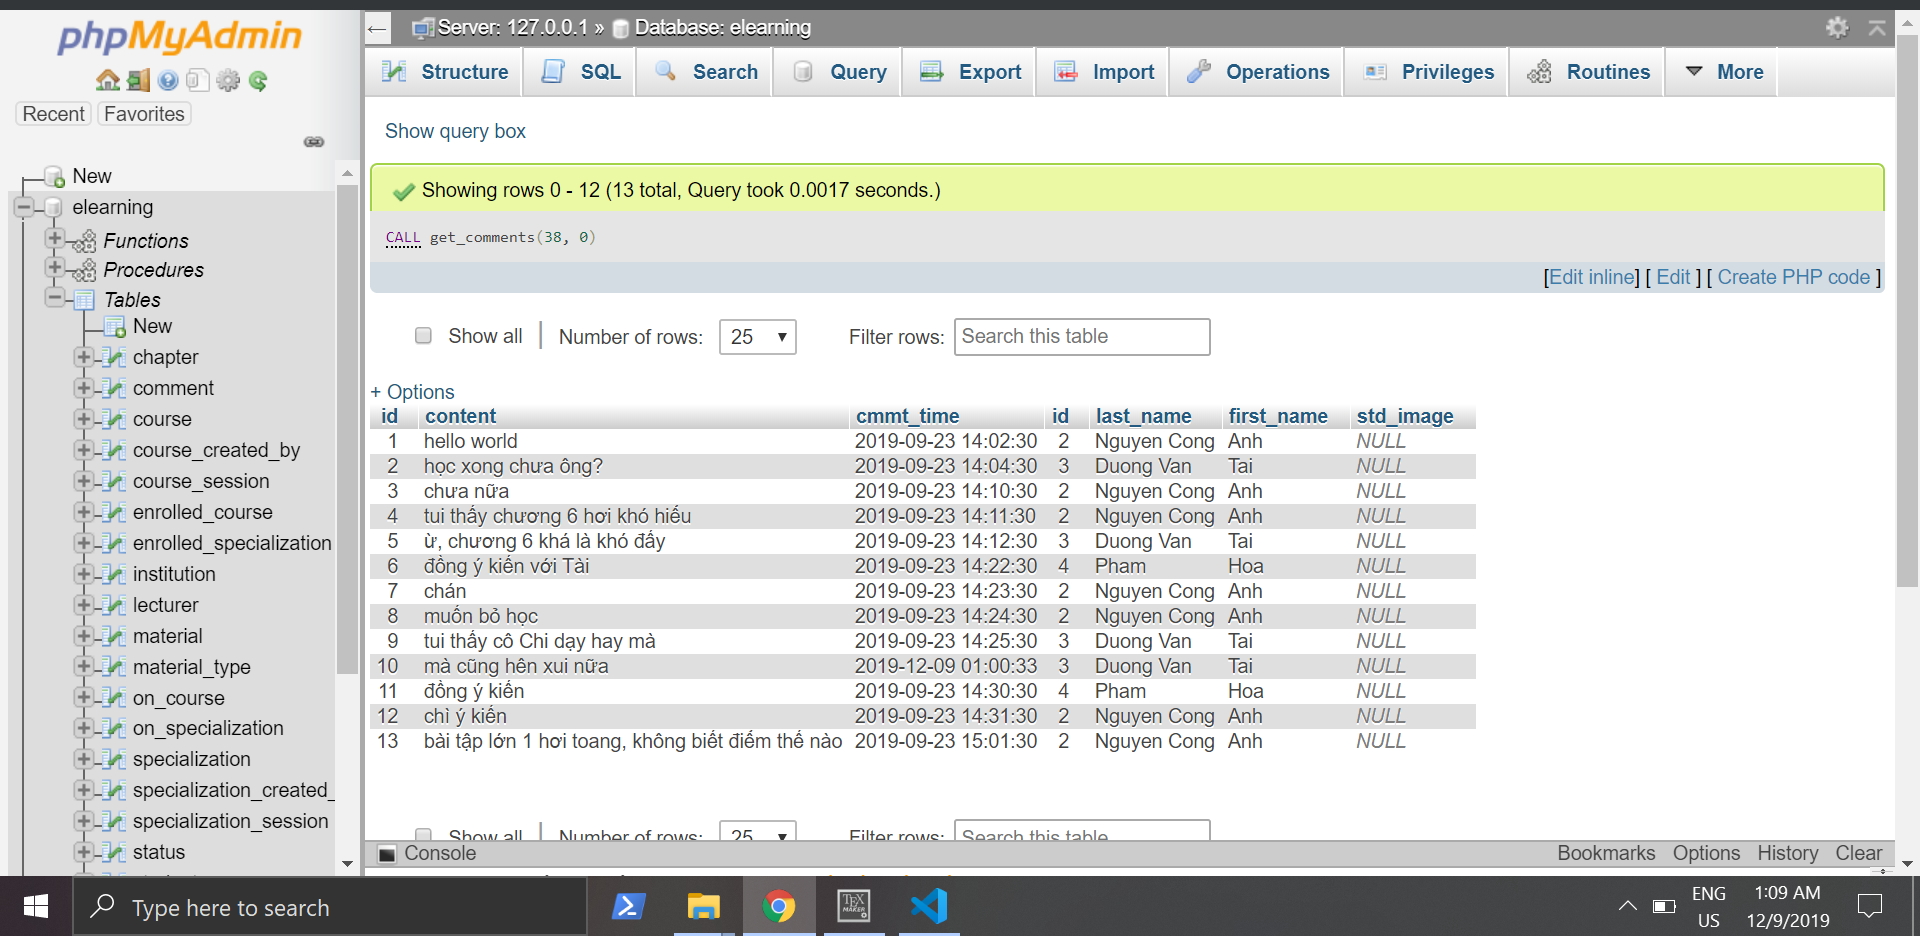
\includegraphics[width=0.8\textwidth]{images/cmmt5.png}
\end{figure}
\subsubsection{Thủ tục chứa câu truy vấn 2}
\textbf{$\bullet$ Mô tả chức năng:} Thủ tục nhận vào một mã người học, truy vấn số lượng comment của người học đó nhóm theo các khóa học mà người đó tham gia, sắp thứ tự bởi id của comment.\\
\textbf{$\bullet$ Lệnh tạo thủ tục:}
\begin{lstlisting}
DELIMITER $$
CREATE PROCEDURE student_comment_summary
(
    IN std_id INT
)
BEGIN
	SELECT cmt.student_id AS 'student id', cmt.course_id AS 'course id', COUNT(*) AS 'comments' 
	FROM `comment` AS cmt
	WHERE cmt.student_id = std_id
    GROUP BY cmt.course_id
	ORDER BY cmt.id;
END $$
DELIMITER ;
\end{lstlisting}
\textbf{$\bullet$ Lệnh thực thi:}
\begin{lstlisting}
CALL student_comment_summary(2);
\end{lstlisting}
\textbf{$\bullet$ Kết quả:}
\begin{figure}[h!]
	\centering
	\caption{Tổng kết số comment của người học trong các khóa học của họ}
	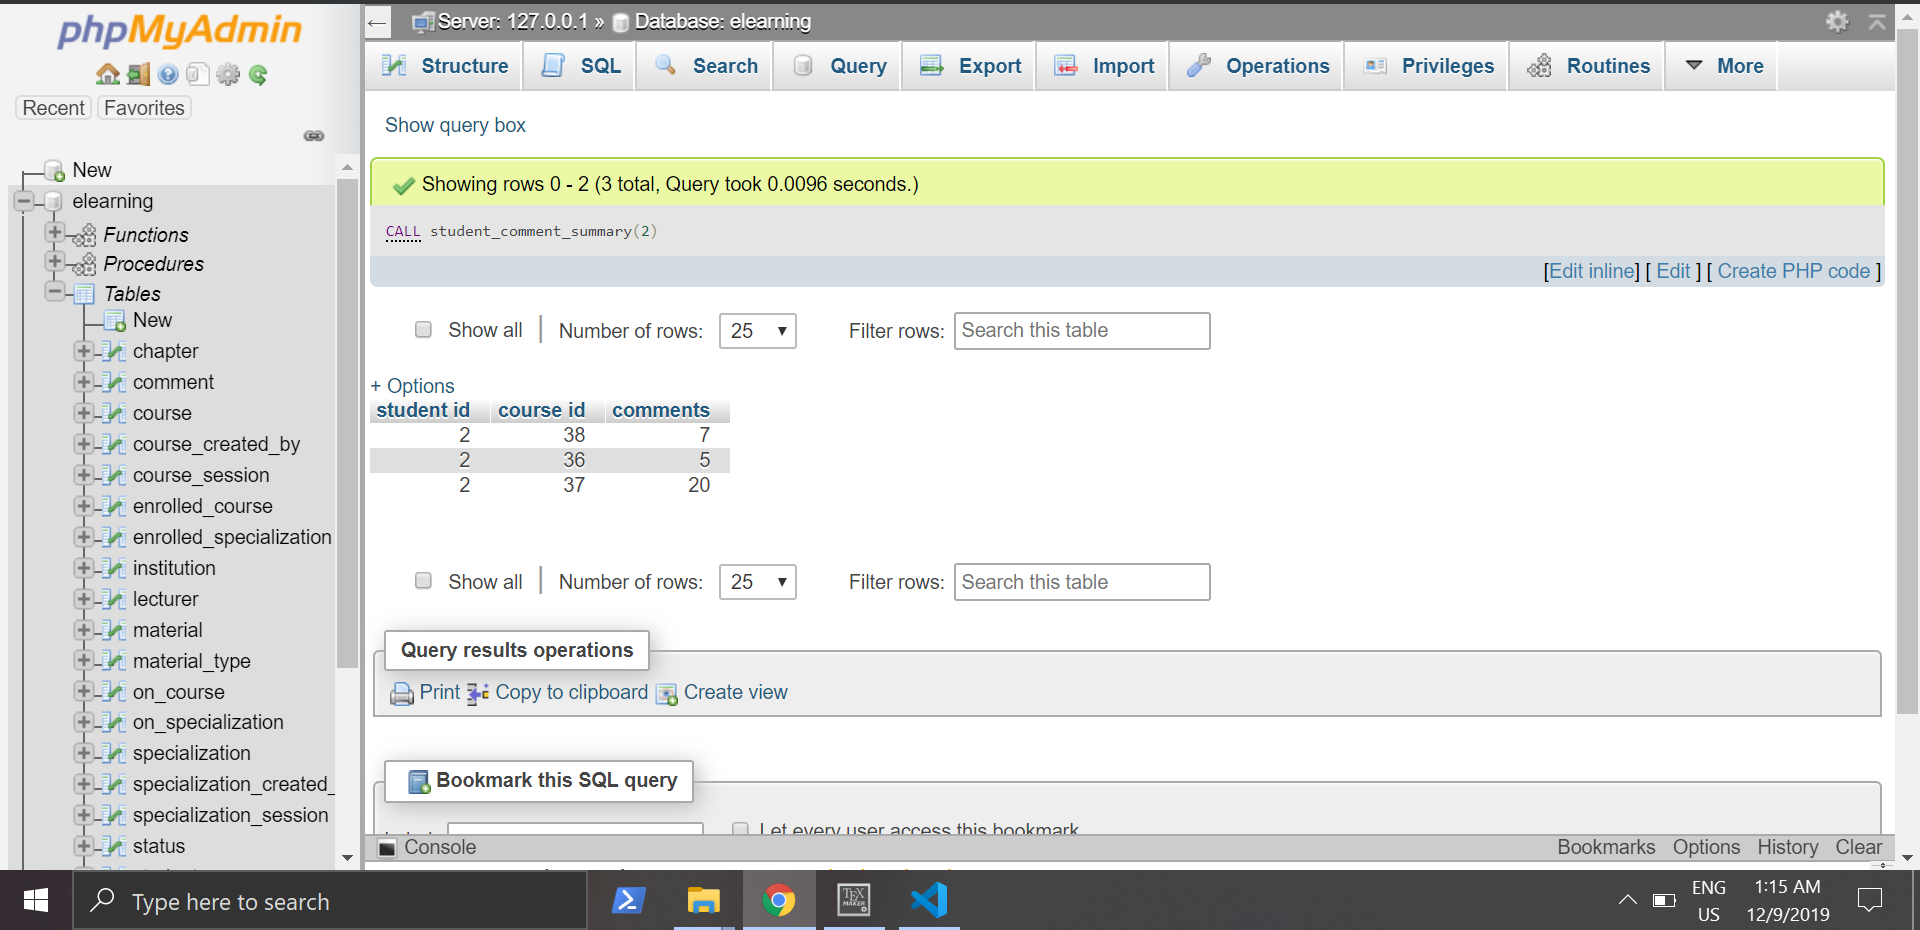
\includegraphics[width=0.8\textwidth]{images/cmmt6.png}
\end{figure}
\subsubsection{Hàm 1}
\textbf{$\bullet$ Mô tả chức năng:} Hàm nhận vào một mã số người học và một mã số khóa học, hiển thị số lượng comment của người học hiện tại trong khóa học đó.\\
\textbf{$\bullet$ Lệnh tạo hàm:}
\begin{lstlisting}
DELIMITER $$
CREATE FUNCTION count_comment(std_id INT, crs_id INT) RETURNS INT
BEGIN
  DECLARE count_cmt INT DEFAULT 0;
  --
  IF ((SELECT COUNT(*) FROM `student` WHERE id = std_id) = 0)
  THEN
    SIGNAL SQLSTATE '45000'
	  SET MESSAGE_TEXT = 'student not found';
  END IF;
  --
  IF ((SELECT COUNT(*) FROM `course` WHERE id = crs_id) = 0)
  THEN
    SIGNAL SQLSTATE '45000'
	  SET MESSAGE_TEXT = 'course not found';
  END IF;
  SET count_cmt = (SELECT COUNT(*) FROM `comment` WHERE student_id = std_id AND course_id = crs_id);
  RETURN count_cmt;
END $$
DELIMITER ;
\end{lstlisting}
\textbf{$\bullet$ Câu lệnh SELECT minh họa gọi hàm:}
\begin{lstlisting}
SELECT *
FROM `student` AS std, `course` AS crs
WHERE count_comment(std.id, crs.id) > 5
\end{lstlisting}
\textbf{$\bullet$ Kết quả:}
\begin{figure}[h!]
	\centering
	\caption{Các khóa học có người học comment nhiều hơn 5 lần}
	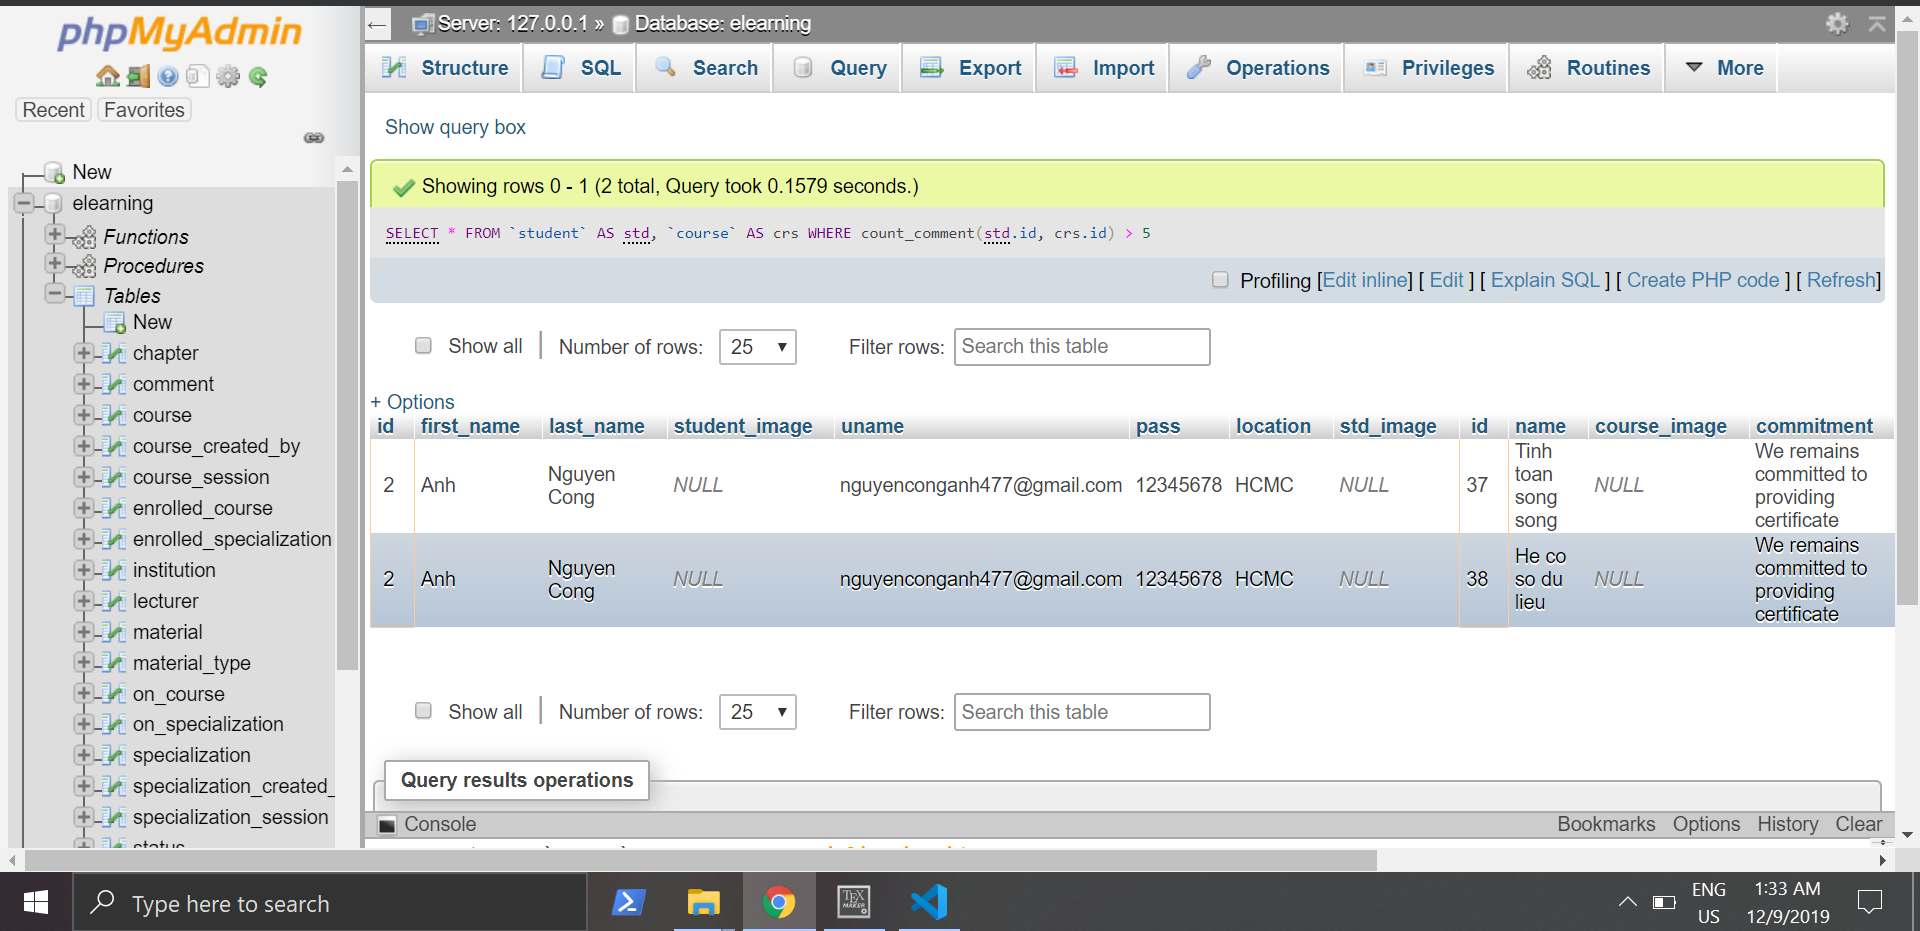
\includegraphics[width=0.8\textwidth]{images/cmmt7.png}
\end{figure}
\subsubsection{Hàm 2}
\textbf{$\bullet$ Mô tả chức năng:} Hàm có input là gmail của người học, kiểm tra người học đó có bao giờ comment chứa chữ "h" hay không.\\
\textbf{$\bullet$ Lệnh tạo hàm:}
\begin{lstlisting}
SET GLOBAL log_bin_trust_function_creators = 1
DROP FUNCTION IF EXISTS `total_comment_user_contain_h_character`$$
CREATE FUNCTION total_comment_user_contain_h_character(fusername varchar(255)) 
RETURNS INT
BEGIN
	declare flag INT(11) default 0 ;
	IF exists(select * from student where student.uname = fusername) 
    THEN
        select count(if(content like '%h%',1,NULL)) into flag from comment,student 
        where student.id = comment.student_id 
        and student.uname = fusername;
		return flag;
    ELSE 		
        SIGNAL SQLSTATE '45000' SET MESSAGE_TEXT = 'TAI KHOAN KHONG TON TAI';
    END IF;
END $$
DELIMITER ;
\end{lstlisting}
\textbf{$\bullet$ Câu lệnh SELECT minh họa gọi hàm:}
\begin{lstlisting}
SELECT total_comment_user_contain_h_character('nguyenconganh477@gmail.com')
\end{lstlisting}
\textbf{$\bullet$ Kết quả:}
\begin{figure}[h!]
	\centering
	\caption{Kiểm tra người dùng nguyenconganh477@gmail.com}
	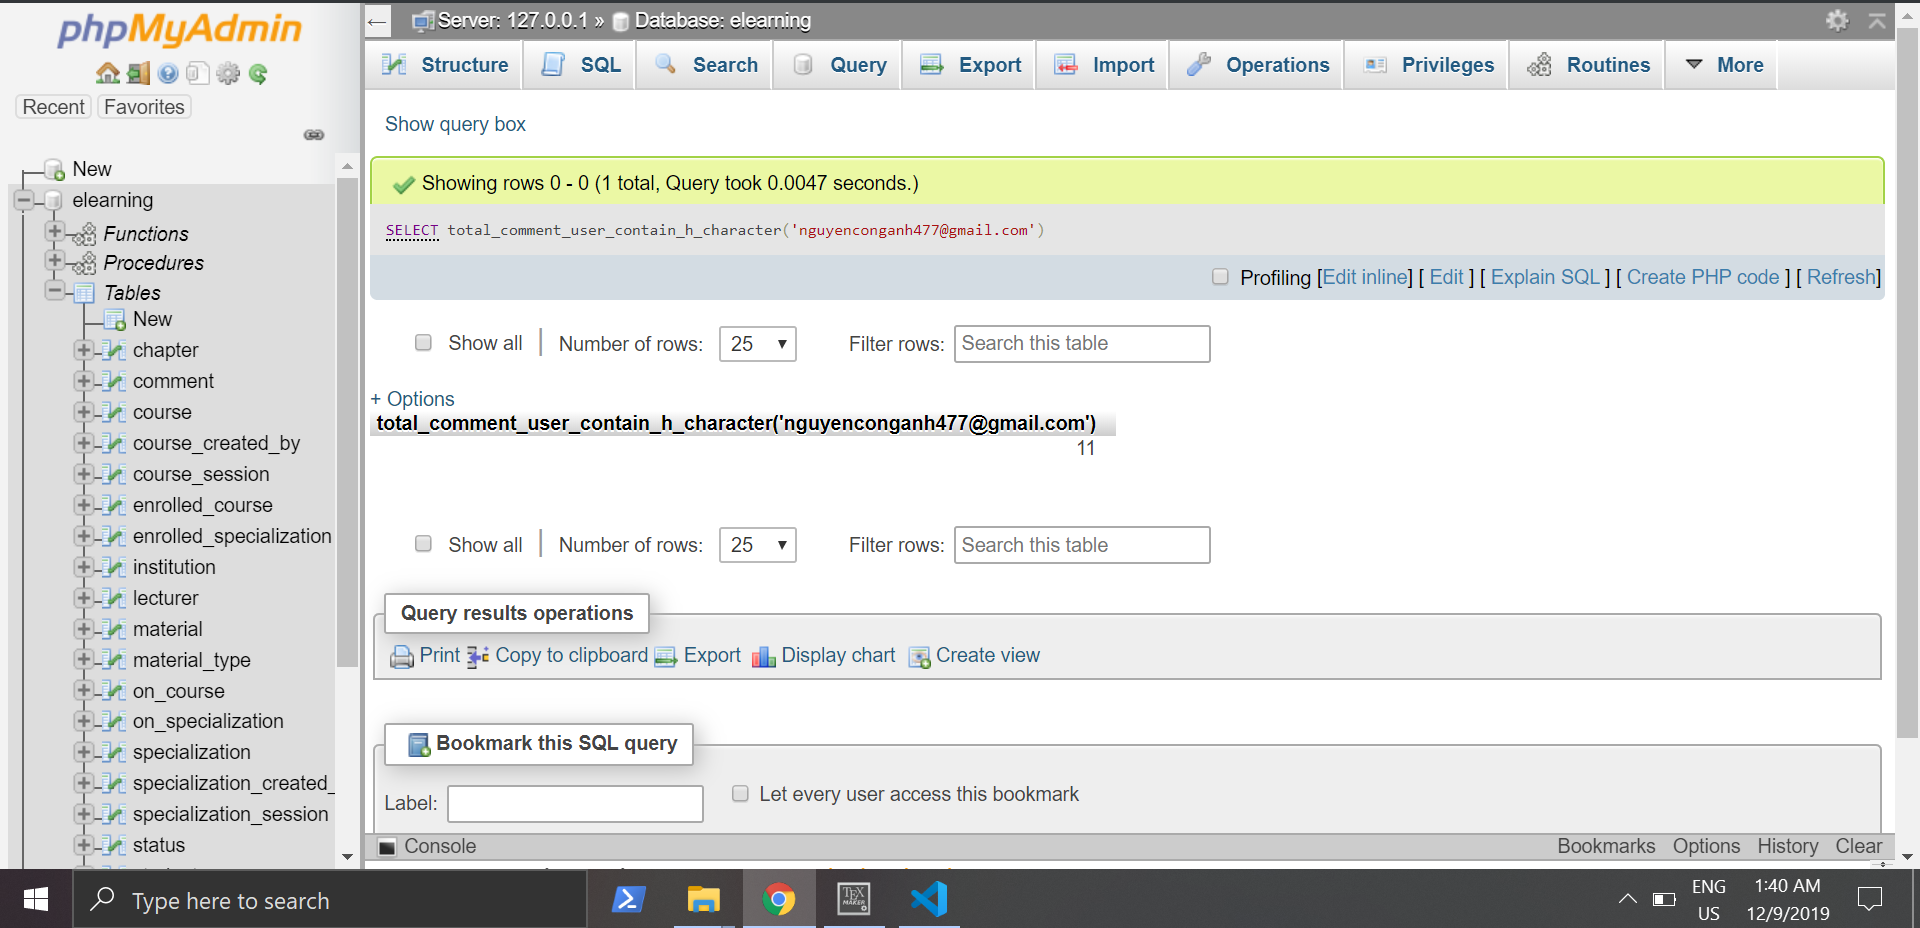
\includegraphics[width=0.8\textwidth]{images/cmmt8.png}
\end{figure}
\subsubsection{Giao diện ứng dụng và các hình ảnh minh họa}
\newpage
\begin{figure}[h!]
	\centering
	\caption{Danh sách các comment}
	
\includegraphics[width=0.4\textwidth]{images/comment1.png}
\end{figure}
\newpage
\subsection{Thao tác với bảng dữ liệu student}
\textit{Thành viên 3: Phạm Hòa, MSSV: 1711440}
\subsubsection{Thủ tục Insert dữ liệu}
\textbf{$\bullet$ Mô tả chức năng:} Thêm tài khoản student vào bảng. Kiểm tra tài khoản có tồn tại hay không. \\
\textbf{$\bullet$ Lệnh tạo thủ tục:}
\begin{lstlisting}
DELIMITER $$
DROP PROCEDURE IF EXISTS `insertUser`$$
CREATE PROCEDURE insertUser
           (IN first_name varchar(64),
           IN last_name varchar(64),
           IN image_url text ,
           IN user_name varchar(255),
           IN password varchar(255),
           IN location text,
           OUT result VARCHAR(255)
           )
 BEGIN
	IF exists(select * from student where student.uname=user_name)  THEN 
		SET result = ' tai khoan da ton tai';
	ELSE 
		INSERT INTO `student`(`id`,`first_name`,`last_name`,`image_url`,`uname`,`pass`,`location`)
			VALUES
			(null,first_name,last_name,image_url,user_name,password,location);
		SET result = ' insert thanh cong';
	END IF ;
END$$
\end{lstlisting}
\textbf{$\bullet$ Lệnh thực thi:}
\begin{lstlisting}
call insertUser('pham','hoa','image','uname123','pass','gialai',@r);
select @r;
\end{lstlisting}
\textbf{$\bullet$ Kết quả:}
\begin{figure}[h!]
	\centering
	\caption{Insert user thành công}
	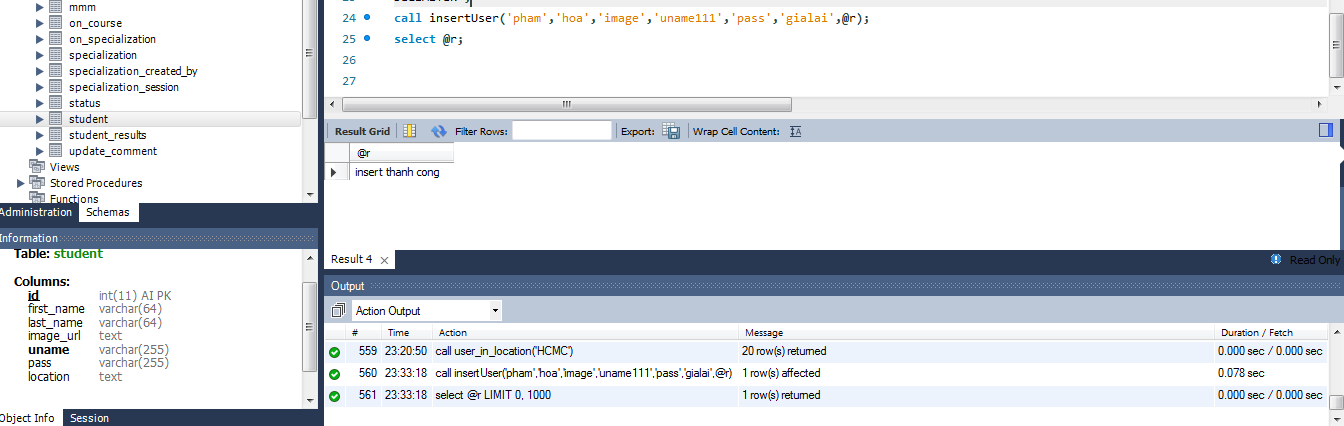
\includegraphics[width=0.8\textwidth]{images/image5.png}
\end{figure}
\begin{figure}[h!]
	\centering
	\caption{Insert user thất bại}
	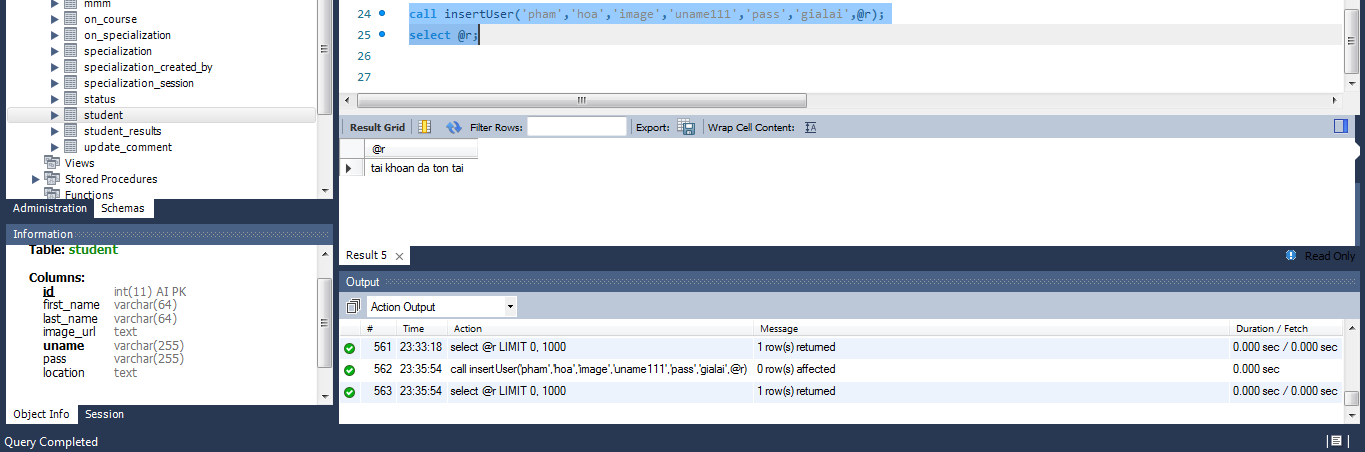
\includegraphics[width=0.8\textwidth]{images/image7.png}
\end{figure}
\subsubsection{Trigger delete student}
\textbf{$\bullet$ Mô tả chức năng:} trigger before sẽ xóa các course đã đăng kí.\\
\textbf{$\bullet$ Lệnh tạo trigger:}
\begin{lstlisting}
DELIMITER $$
DROP TRIGGER IF EXISTS `delete_student`$$
create trigger delete_student 
	BEFORE delete on student 
    FOR EACH ROW
BEGIN
		DELETE p1 
        FROM enrolled_course p1
        WHERE student_id = OLD.id;
        DELETE p1 
        FROM enrolled_specialization p1
        WHERE student_id = OLD.id;
END;
$$
DELIMITER ;
\end{lstlisting}
\textbf{$\bullet$ Lệnh kiểm tra trigger hoạt động:}
\subsubsection{Trigger number student deleted}
\textbf{$\bullet$ Mô tả chức năng:} Biến n_account_delete sẽ đếm bao nhiêu tài khoản đã bị xóa.\\
\textbf{$\bullet$ Lệnh tạo trigger:}
\begin{lstlisting}
set @n_account_delete = 0;
DELIMITER $$
DROP TRIGGER IF EXISTS `number_student_deleted`$$
create trigger number_student_deleted
	AFTER delete on student
FOR EACH ROW
BEGIN
	SET @n_account_delete = @n_account_delete+1;
END    
$$
DELIMITER ;
\end{lstlisting}
\textbf{$\bullet$ Lệnh kiểm tra trigger hoạt động:}
\begin{lstlisting}
from student p1
where id = 19;
select @n_account_delete;
\end{lstlisting}
\textbf{$\bullet$ Kết quả:}
\begin{figure}[h!]
	\centering
	\caption{Sau khi delete 1 student}
	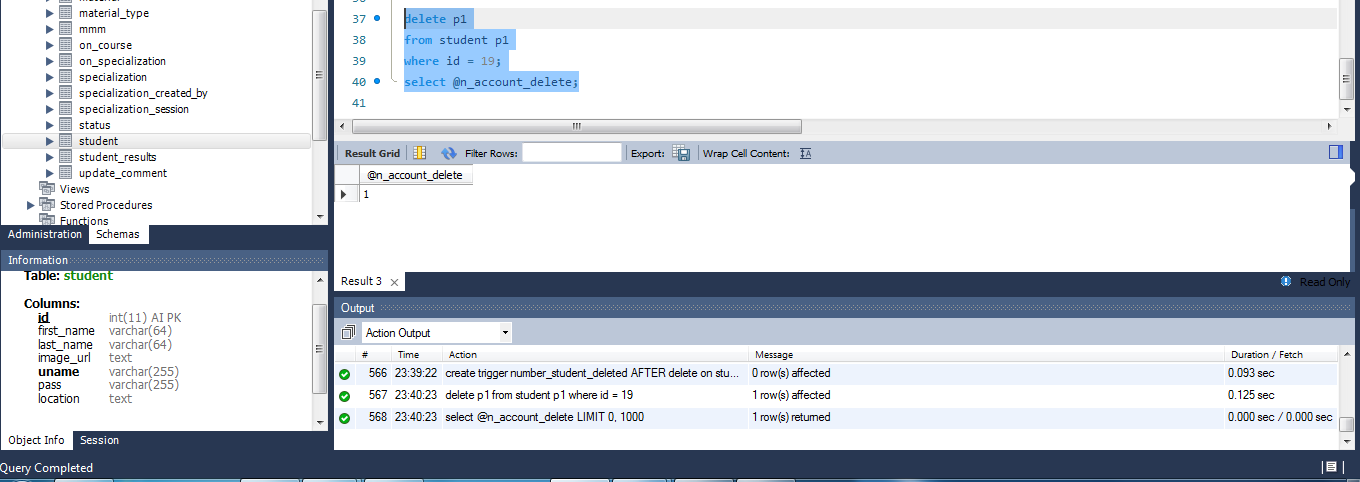
\includegraphics[width=0.8\textwidth]{images/image6.png}
\end{figure}
\subsubsection{Thủ tục chứa câu truy vấn 1}
\textbf{$\bullet$ Mô tả chức năng:} Hiện danh sách các username có số lần đăng kí các khóa học lớn hơn số N cho trước.\\
\textbf{$\bullet$ Lệnh tạo thủ tục:}
\begin{lstlisting}
DELIMITER $$
DROP PROCEDURE IF EXISTS `number_course_users_more_than`$$
CREATE PROCEDURE number_course_users_more_than(IN num INT)
BEGIN
    -- SELECT COUNT(*) INTO flag FROM student, enrolled_course WHERE user_name = username and student.id=enrolled_course.student_id;
    SELECT uname,count(*) -- into listname,number 
		from student,enrolled_course 
		where student.id = enrolled_course.student_id 
		GROUP BY uname having count(*) > num ORDER BY count(*) DESC;
END;
$$
DELIMITER ;
\end{lstlisting}
\textbf{$\bullet$ Lệnh thực thi:}
\begin{lstlisting}
call number_course_users_more_than(1);
\end{lstlisting}
\textbf{$\bullet$ Kết quả:}
\newpage
\begin{figure}[h!]
	\centering
	\caption{Kết quả lệnh call procedure}
	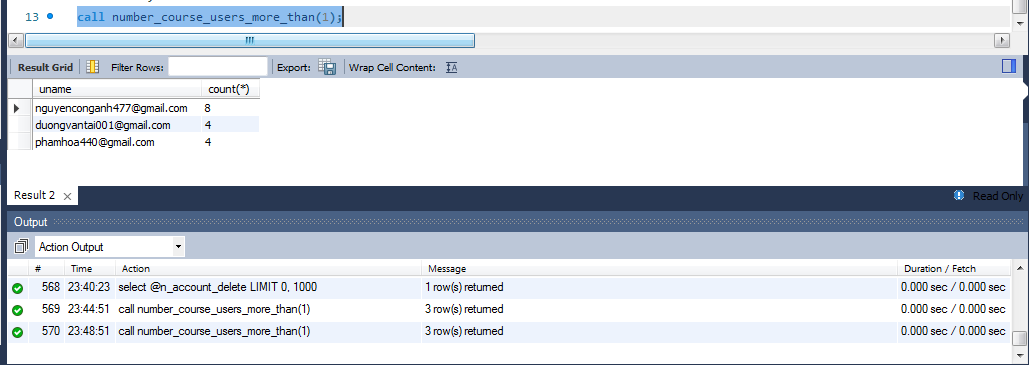
\includegraphics[width=0.8\textwidth]{images/image9.png}
\end{figure}
\subsubsection{Thủ tục chứa câu truy vấn 2}
\textbf{$\bullet$ Mô tả chức năng:} Hiển thị danh sách các user ở vị trí cho trước. \\
\textbf{$\bullet$ Lệnh tạo thủ tục:}
\begin{lstlisting}
DELIMITER $$
DROP PROCEDURE IF EXISTS `user_in_location`$$
CREATE PROCEDURE user_in_location(IN loc text)
BEGIN
    SELECT uname
		from student
		where student.location = loc;
END;
$$
DELIMITER ;

\end{lstlisting}
\textbf{$\bullet$ Lệnh thực thi:}
\begin{lstlisting}
call user_in_location('HCMC')
\end{lstlisting}
\textbf{$\bullet$ Kết quả:}
\begin{figure}[h!]
	\centering
	\caption{Danh sách các user có location là HCMC}
	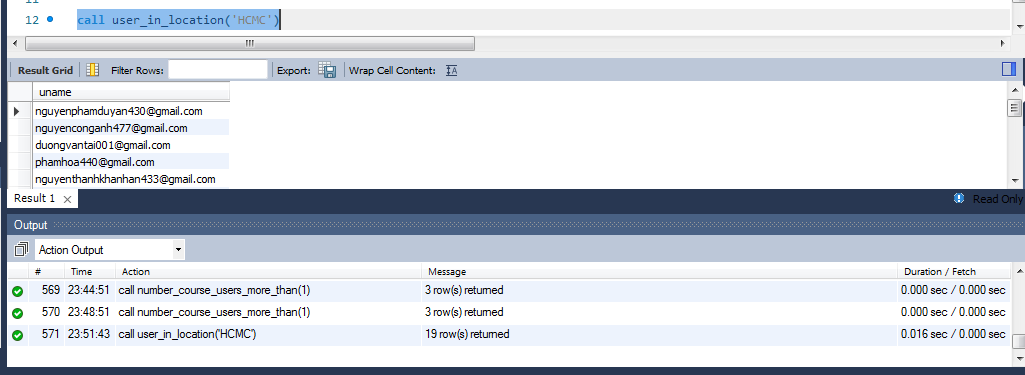
\includegraphics[width=0.8\textwidth]{images/image8.png}
\end{figure}
\subsubsection{Hàm 1}
\textbf{$\bullet$ Mô tả chức năng:} Hiển danh số lượng khóa học của 1 student cho trước. Kiểm tra user có tồn tại không.\\
\textbf{$\bullet$ Lệnh tạo hàm:}
\begin{lstlisting}
DELIMITER $$
DROP FUNCTION IF EXISTS `number_course`$$
CREATE FUNCTION number_course(username VARCHAR(255))
RETURNS INT
BEGIN
	DECLARE flag INT(11) DEFAULT 0;
	if exists(select * FROM student WHERE uname = username) THEN
		SELECT COUNT(*) INTO flag FROM student, enrolled_course WHERE student.uname = username and student.id=enrolled_course.student_id;
		RETURN flag;
	ELSE
		SIGNAL SQLSTATE '45000' SET MESSAGE_TEXT = 'TAI KHOAN KHONG TON TAI';
    END IF;
END;
$$
DELIMITER ;
\end{lstlisting}
\textbf{$\bullet$ Câu lệnh SELECT minh họa gọi hàm:}
\begin{lstlisting}
SELECT number_course('nguyenconganh477@gmail.com');
SELECT number_course('khongtontai@gmail.com');
\end{lstlisting}
\textbf{$\bullet$ Kết quả:}
\begin{figure}[h!]
	\centering
	\caption{tồn tại user}
	\includegraphics[width=0.8\textwidth]{images/image2.png}
\end{figure}
\begin{figure}[h!]
	\centering
	\caption{kết quả chạy câu lệnh khi không tồn tại user}
	\includegraphics[width=0.8\textwidth]{images/image1.png}
\end{figure}
\subsubsection{Hàm 2}
\textbf{$\bullet$ Mô tả chức năng:} Đếm tổng số tiền mà 1 user đã sử dụng đẻ mua khóa học. Kiểm tra user có tồn tại không. Hiển danh sách số lượng khóa học của 1 student cho trước. \\
\textbf{$\bullet$ Lệnh tạo hàm:}
\begin{lstlisting}
DELIMITER $$
DROP FUNCTION IF EXISTS `payed_of_user`$$
CREATE FUNCTION payed_of_user(username VARCHAR(255))
RETURNS decimal(8,2)
BEGIN
	DECLARE flag INT(11) DEFAULT 0;
	if exists(select * FROM student WHERE uname = username) THEN
		SELECT sum(course_price) into flag FROM student, enrolled_course,course_session,course
			WHERE uname = username
			and student.id=enrolled_course.student_id
			and course_session_id=course_session.id
			and course_id = course.id;
		RETURN flag;
	ELSE
		SIGNAL SQLSTATE '45000' SET MESSAGE_TEXT = 'TAI KHOAN KHONG TON TAI';
    END IF;
END;
$$
DELIMITER ;
\end{lstlisting}
\textbf{$\bullet$ Câu lệnh SELECT minh họa gọi hàm:}
\begin{lstlisting}
select payed_of_user('nguyenconganh477@gmail.com');
select payed_of_user('khongtontai@gmail.com');
\end{lstlisting}
\textbf{$\bullet$ Kết quả:}
\begin{figure}[h!]
	\centering
	\caption{kết quả gọi function thành công}
	\includegraphics[width=0.8\textwidth]{images/image4.png}
\end{figure}
\begin{figure}[h!]
	\centering
	\caption{kết quả gọi function với user không tồn tại trong data}
	\includegraphics[width=0.8\textwidth]{images/image3.png}
\end{figure}
\newpage
\subsubsection{Giao diện ứng dụng và các hình ảnh minh họa}
\begin{figure}[h!]
	\centering
	\caption{Profile user}
	\includegraphics[width=0.35\textwidth]{images/user1.png}
\end{figure}
\begin{figure}[h!]
	\centering
	\caption{Delete user}
	\includegraphics[width=0.35\textwidth]{images/user2.png}
\end{figure}
\newpage
\begin{figure}[h!]
	\centering
	\caption{Đăng xuất}
	\includegraphics[width=0.35\textwidth]{images/user3.png}
\end{figure}
\subsection{Database Diagram}
\begin{figure}[h!]
	\centering
	\caption{Database Diagram}
	\includegraphics[width=1.0\textwidth]{images/dbs.png}
\end{figure}
\newpage
\section{Phụ lục}
\subsection{Báo cáo bài tập lớn số 1}
\subsubsection{Thu thập và phân tích yêu cầu (phiên bản cũ):}
\textbf{Các đối tượng dữ liệu cần lưu và các thuộc tính}\\
Một hệ thống e-learning cần lưu thông tin của các đối tác (partners), các đối tác sẽ cung cấp các khóa học (courses) và các lộ trình (specializations) cho hệ thống. Một đối tác có thể là một công ty (company partner) hoặc một trường đại học (university partner), cũng có thể là một cá nhân hay một tổ chức nào khác,... Mỗi đối tác có một tên duy nhất, một số điện thoại, nhiều email và nhiều địa chỉ nếu đối tác có nhiều chi nhánh, ngoài ra cần lưu thêm một phần giới thiệu ngắn về đối tác. Mỗi đối tác sẽ được hệ thống cấp cho một id duy nhất, một tài khoản duy nhất để đăng nhập vào hệ thống. Nếu đối tác là một trường đại học thì cần lưu thêm quốc gia của trường đại học đó, nếu là một công ty thì cần lưu thêm loại công ty và số lượng nhân viên hiện tại của công ty đó. Ngoài ra với mỗi đối tác, có thể lưu các thông tin về chủ tịch của đối tác đó, bao gồm tên chủ tịch, một số điện thoại và một email để liên lạc khi cần thiết.\\\\
Một khóa học sẽ có tên khóa học, mô tả khái quát về khóa học, các ngôn ngữ được dùng để dạy trong khóa học và phí đăng ký. Một khóa học có thể có các mùa, mùa hiện tại của khóa học được lưu bằng ngày bắt đầu và ngày kết thúc của mùa. Ngoài ra đối với mỗi khóa học, cần lưu cấp độ của khóa học, điểm sàn được yêu cầu để hoàn thành khóa học, trạng thái khóa học có mở hay không, khóa học có cung cấp chứng chỉ khi hoàn thành hay không và điểm đánh giá của người học về khóa học đó. Mỗi khóa học khi được cung cấp sẽ được hệ thống cấp cho một id duy nhất.\\\\
Lộ trình là một tổ hợp của các khóa học có liên quan đến một chuyên ngành nào đó, khi một lộ trình được cung cấp, hệ thống sẽ cấp cho nó một id duy nhất. Hệ thống cần lưu tên của lộ trình, mô tả khái quát về lộ trình, phí đăng ký, có cung cấp chứng chỉ khi hoàn thành hay không và điểm đánh giá của người học về lộ trình.\\\\
Mỗi người dùng hệ thống (user) có một tài khoản duy nhất, một người dùng chỉ có thể là một tổ chức (institution) hoặc một người học (student). Với người học, cần lưu tên, id duy nhất, các chuyên ngành của người học, các ngôn ngữ người học sử dụng, ngày sinh và một địa chỉ email. Với tổ chức, cần lưu tên, id duy nhất, một địa chỉ email và địa chỉ trụ sở chính. Ngoài ra còn có các team, mỗi team có một id duy nhất và một tên nhóm.\\
Mỗi giảng viên (lecturer) có tên, một tài khoản duy nhất, một id duy nhất, bậc học, nhiều email và một phần giới thiệu sơ lược về giảng viên đó.\\\\
Các chương (chapters) trong một khóa học có tên khác nhau, có thời gian để hoàn thành và mô tả khái quát.\\\\
Hệ thống lưu các dự án, dự án (project) có tên và một số hiệu duy nhất. Bài tập lớn cuối mỗi khóa học cũng tương tự dự án nhưng lượng công việc ít hơn.\\
Video bài giảng, bài đọc, bài kiểm tra và bài tập đều có một số hiệu duy nhất. Mỗi video có tên, kịch bản, ngôn ngữ, thời lượng và danh sách các giảng viên dạy.\\\\
Mỗi bài đọc có tên và các tác giả. Mỗi bài kiểm tra có tên, cấp độ, số lượng câu hỏi, số điểm thấp nhất để hoàn thành. Mỗi bài tập có tên, cấp độ, mô tả và yêu cầu.\\\\
Các forum được lưu với một số hiệu duy nhất, có chủ đề của forum, trạng thái hiện tại và số lượng comment hiện tại.\\\\
Các bản ghi kết quả (record) và các chứng chỉ có một số hiệu duy nhất. Đối với chứng chỉ, có tên trường đại học, tên khóa học, tên người học và ngày được nhận. Đối với bản ghi kết quả, có tên khóa học, danh sách giảng viên, tên trường đại học, điểm cuối cùng, thời gian hoàn thành và ngày hoàn thành.\\\\
\textbf{Mối liên kết giữa các đối tượng}\\
Đối tác cung cấp khóa học.\\
Đối tác cung cấp lộ trình.\\
Chủ tịch quản lý đối tác.\\
Đối tác đại học cung cấp chứng chỉ.\\
Người học đạt được chứng chỉ.\\
Tổ chức đào tạo người học.\\
Bảng kết quả học thuộc về người học.\\
Bảng kết quả học thuộc về nhóm người học.\\
Người học thuộc về nhóm người học.\\
Giảng viên dạy trong khóa học.\\
Giảng viên dạy trong lộ trình.\\
Lộ trình bao gồm khóa học.\\
Lộ trình bao gồm lộ trình.\\
Lộ trình yêu cầu dự án.\\
Khóa học yêu cầu dự án nhỏ.\\
Người học đăng ký khóa học.\\
Người học đăng ký lộ trình.\\
Khóa học có chương học.\\
Chương học có video bài giảng.\\
Chương học có tài liệu đọc.\\
Chương học có bài kiểm tra.\\
Chương học có bài tập.\\
Chương học có diễn đàn.\\\\
\textbf{Các ràng buộc cần có}\\
Một đối tác phải cung cấp ít nhất một khóa học, còn lộ trình là không bắt buộc; có thể cung cấp nhiều khóa học, nhiều lộ trình. Một khóa học hoặc lộ trình bắt buộc phải thuộc về một đối tác duy nhất. Một đối tác chỉ do một chủ tịch quản lý.\\\\
Một khóa học có thể có trong nhiều lộ trình, một lộ trình có từ một đến nhiều khóa học, trong một lộ trình cũng có thể có các lộ trình khác.
Một giảng viên phải dạy trong ít nhất một khóa học, còn lộ trình là không bắt buộc; có thể dạy trong nhiều khóa học, nhiều lộ trình. Một khóa học hoặc lộ trình phải có giảng viên dạy, từ một đến nhiều giảng viên.\\\\
Một người dùng có thể đăng ký các khóa học và lộ trình hoặc không, một khóa học hoặc lộ trình có thể được mọi người đăng ký hoặc không.\\\\
Một đối tác đại học có thể cung cấp nhiều chứng chỉ nhưng không bắt buộc, một người học có thể có nhiều chứng chỉ cũng có thể không có chứng chỉ nào. Một chứng chỉ bắt buộc phải do một đối tác đại học cấp, bắt buộc phải thuộc về một người học.\\\\
Một tổ chức có thể đang đào tạo nhiều người học hoặc không đào tạo người nào, một người học có thể thuộc nhiều tổ chức nhưng không bắt buộc thuộc tổ chức nào.\\\\
Một người học hoặc một nhóm người học có thể có nhiều bảng kết quả học, một nhóm người học có thể có nhiều người học.\\\\
Một khóa học phải có từ một đến nhiều chương, mỗi chương học có thể có hoặc không có các video bài giảng, tài liệu đọc, bài kiểm tra, bài tập, diễn đàn. Các tài nguyên này nếu có phải thuộc về duy nhất chương đó, ngoại trừ tài liệu đọc có thể thuộc về nhiều chương.\\\\
Một lộ trình có thể có nhiều dự án, một dự án phải thuộc về duy nhất một lộ trình. Một khóa học có thể có một dự án nhỏ cuối khóa, một dự án nhỏ phải thuộc về duy nhất một khóa học.\\\\
\textbf{Các nghiệp vụ chính}\\
Hệ thống cho phép đối tác:\\
Đăng nhập\\
Thêm, xóa, chỉnh sửa các khóa học và các lộ trình\\
Thêm, xóa, chỉnh sửa các chứng chỉ\\
Thống kê số lượng mua khóa học theo người học, theo tổ chức\\
Thống kê số tiền thu được\\\\
Hệ thống cho phép tổ chức:\\
Đăng ký tài khoản, đăng nhập\\
Đăng ký khóa học và lộ trình\\
Thanh toán bằng thẻ\\
Thêm, xóa, chỉnh sửa danh sách học viên mình đào tạo\\
Đánh giá khóa học và lộ trình\\
Xem kết quả học tập của các học viên\\\\
Hệ thống cho phép người học:\\
Đăng ký tài khoản, đăng nhập\\
Đăng ký khóa học và lộ trình\\
Thanh toán bằng thẻ\\
Đăng ký nhóm học tập\\
Xem lại kết quả học tập\\
Xem thông tin chứng chỉ\\\\
Hệ thống cho phép giảng viên:\\
Đăng ký tài khoản, đăng nhập\\
Chỉnh sửa các khóa học và lộ trình do mình dạy\\\\
\textbf{Các ràng buộc ngữ nghĩa mà không biểu diễn được bằng (E-)ERD}\\
Phí đăng ký của một lộ trình phải nhỏ hơn tổng phí đăng ký của các khóa học thuộc lộ trình đó để tạo ra một khoản chiết khấu cho người đăng ký.
Khi một mùa của khóa học kết thúc, nếu người học chưa hoàn thành được khóa học thì kết quả đến thời điểm hiện tại sẽ bị hủy, người học phải chờ một mùa mới để có thể học lại từ đầu.\\\\
Người học thuộc một tổ chức có thể sử dụng các khóa học và lộ trình mà tổ chức đó đăng ký. Do đó, phí đăng ký khóa học và lộ trình của một tổ chức không phải phí gốc của khóa học và lộ trình đó mà được tính dựa trên số lượng người học có trong tổ chức.
\subsubsection{Vẽ (E-)ERD (đã chỉnh sửa)}
\newpage
\begin{figure}[h!]
	\centering
	\caption{ERD mới}
	\includegraphics[width=1.0\textwidth]{images/newerd.png}
\end{figure}
\subsubsection{Ánh xạ sang lược đồ cơ sở dữ liệu (đã chỉnh sửa)}
\newpage
\begin{figure}[h!]
	\centering
	\caption{Mapping mới}
	\includegraphics[width=1.0\textwidth]{images/map.png}
\end{figure}
\subsection{Source code chương trình}
\href{https://github.com/imbaggaarm/dbms_assigment_ios}{Ứng dụng}: https://github.com/imbaggaarm/dbms_assigment_ios\\
\href{https://github.com/imbaggaarm/dbms_assignment_go_server}{Server}: https://github.com/imbaggaarm/dbms_assignment_go_server
\subsection{Bảng phân công nhiệm vụ cho phần chung}
\begin{figure}[h!]
	\centering
	\caption{Phân chia công việc}
	\includegraphics[width=1.0\textwidth]{images/pccv.png}
\end{figure}
\end{document}
